\cleardoublepage

\chapter{Proving the spectral theorem}
\label{chapter:spectral-theorem}

When I started writing this, it was not meant to be a book. I was going for a short explanation of Principal Component Analysis that was simple, but that also didn't skip any steps. I was frustrated with other explanations that leave things out, or require the reader to take things at face value.

This chapter illustrates why that so often happens. In this chapter we will prove the \textbf{spectral theorem}, which we introduced in the previous chapter. This is very much the dark heart of PCA: the one result from which everything else follows, so it pays to understand it properly. The drawback is that the proof of the spectral theorem adds a boatload of preliminaries to the story.

Suddenly, just to understand this one statement, we need to understand \textbf{determinants}, the \textbf{characteristic polynomial}, \textbf{complex numbers, vectors and matrices} and \textbf{the fundamental theorem of algebra}. All interesting, of course, and worth knowing about, but it's a lot of baggage if you just want to know how PCA works. So I decided to move it all into one self-contained chapter. 

\section{Restating the spectral theorem}

In the last chapter, we learned the following.

An \emph{orthogonal matrix} is a square matrix whose columns are mutually orthogonal unit vectors. Equivalently, an orthogonal matrix is a matrix \(\rc{\mbP}\) for which \(\rc{\mbP}^{-1} = \rc{\mbP}^T\).

\index{orthogonal matrix}

Any square matrix \(\bc{\mbA}\) is \emph{orthogonally diagonalizable} if there exists an orthogonal matrix \(\rc{\mbP}\) and a diagonal matrix \(\bc{\mbD}\) such that \(\bc{\mbA} = \rc{\mbP}\bc{\mbD}\rc{\mbP}^T\). A matrix \(\bc{\mbA}\) is symmetric if \(\bc{\mbA} = \bc{\mbA}^T\).

\index{Orthogonally diagonalizable}

\begin{theorem}[The spectral theorem] A matrix is orthogonally diagonalizable if and only if it is symmetric.
\end{theorem}

\begin{aside}We call this ``the'' spectral theorem in the context of this book. In general, there are many spectral theorems about which operators can be diagonalized under which conditions. 
\end{aside}

Previously, we saw how much follows from this one simple theorem. If we take this to be true, we get eigenvectors, whitening and principal components. 

\index{Spectral theorem}

In the rest of this chapter we'll build a toolkit step by step, with which to analyze this problem. At the end, we'll return to the theorem and apply our tools to prove it.

The first is a very useful function of a matrix: the determinant. 

\vspace{4em}

\section{Determinants}

\index{Determinant of a matrix}

The determinant started life long before linear algebra. As early as the 3rd century BCE, the function was used as a property of a set of linear equations that would allow you to determine whether the equations had a solution.

Later, determinants were studied as functions in their own right. In this context, they were seen as very opaque and abstract: something that was useful in higher mathematics, but hard to explain to the lay person. It wasn't until \emph{matrices} become popular, and in particular the view of a matrix as representing a geometric transformation, that determinants finally acquired an intuitive and simple explanation.

That explanation---apart from some subtleties which we'll discuss later---is that for a square matrix \(\bc{\mbA}\), thre determinant expresses how much \(\bc{\mbA}\) \emph{inflates} the space it transforms.

For example, here are three different ways that a matrix might transform space to squish and stretch in different directions.

\begin{figure}[H]
	\centerline{
	\includegraphics[width=1\textwidth]{./images/pca-3/mona-lisa.pdf}
	}
	\caption*{Three linear transformations, showing the effect on the Mona Lisa, and the \bc{unit square}.}
\end{figure}

%<figure class="narrow">
%<img src="/images/pca-3/mona-lisa.svg" />
%<figcaption>
%Three linear transformations, showing the effect on the Mona Lisa, and the <span class="bc">unit square</span>.
%</figcaption>
%</figure>

In the first, everything is stretched equally in all directions by a factor of \(2\). That means that a square with area \(1\) in the original (a \emph{unit} square) has area \(4\) after the transformation by \(\bc{\mbA}\) (since both its sides are doubled). This is what we mean by inflating space: the determinant of \(\bc{\mbA}\) is 4 because transforming something by \(\bc{\mbA}\) increases its area by a factor of 4. In the second example, We stretch by \(1.1\) in one direction, and shrink to \(0.5\) in the other. The result is that that a unit square in the original ends up smaller after the transformation: the determinant of \(\bc{\mbB}\) is \(0.5 \times 1.1 = 0.55\).

\begin{aside}To see that objects other than squares are inflated by the same amount, just subdivide it into small squares. Each of the squares is inflated by the same amount, so the total is as well.
\end{aside}

The third example is a little trickier. The Mona Lisa is again squished and stretched in different directions, but these are not aligned with the axes. The area of the unit square seems to be getting a little smaller, but how can we tell by how much exactly?

Before we dig into the technical details, let's first look at why it is worth doing so. Why is it so important to know by how much a matrix inflates space? There are many answers, but in the context of this series, the most important reason to care about the determinant is that it gives us a very convenient characterization of \emph{invertible matrices}.

\noindent An invertible matrix is simply a matrix whose transformation is invertible. That is, after we apply the transformation \(\mby \leftarrow \bc{\mbA}\mbx\) we can always transform \(\mby\) back to \(\mbx\), and end up where we started. 

When is a matrix not invertible? When multiple inputs \(\mbx\) are mapped to a single output \(\mby\). In linear transformations, this happens when the input is squished so much in one direction, that the resulting space has a lower dimensionality than the original.

\begin{figure}[H]
	\centerline{
	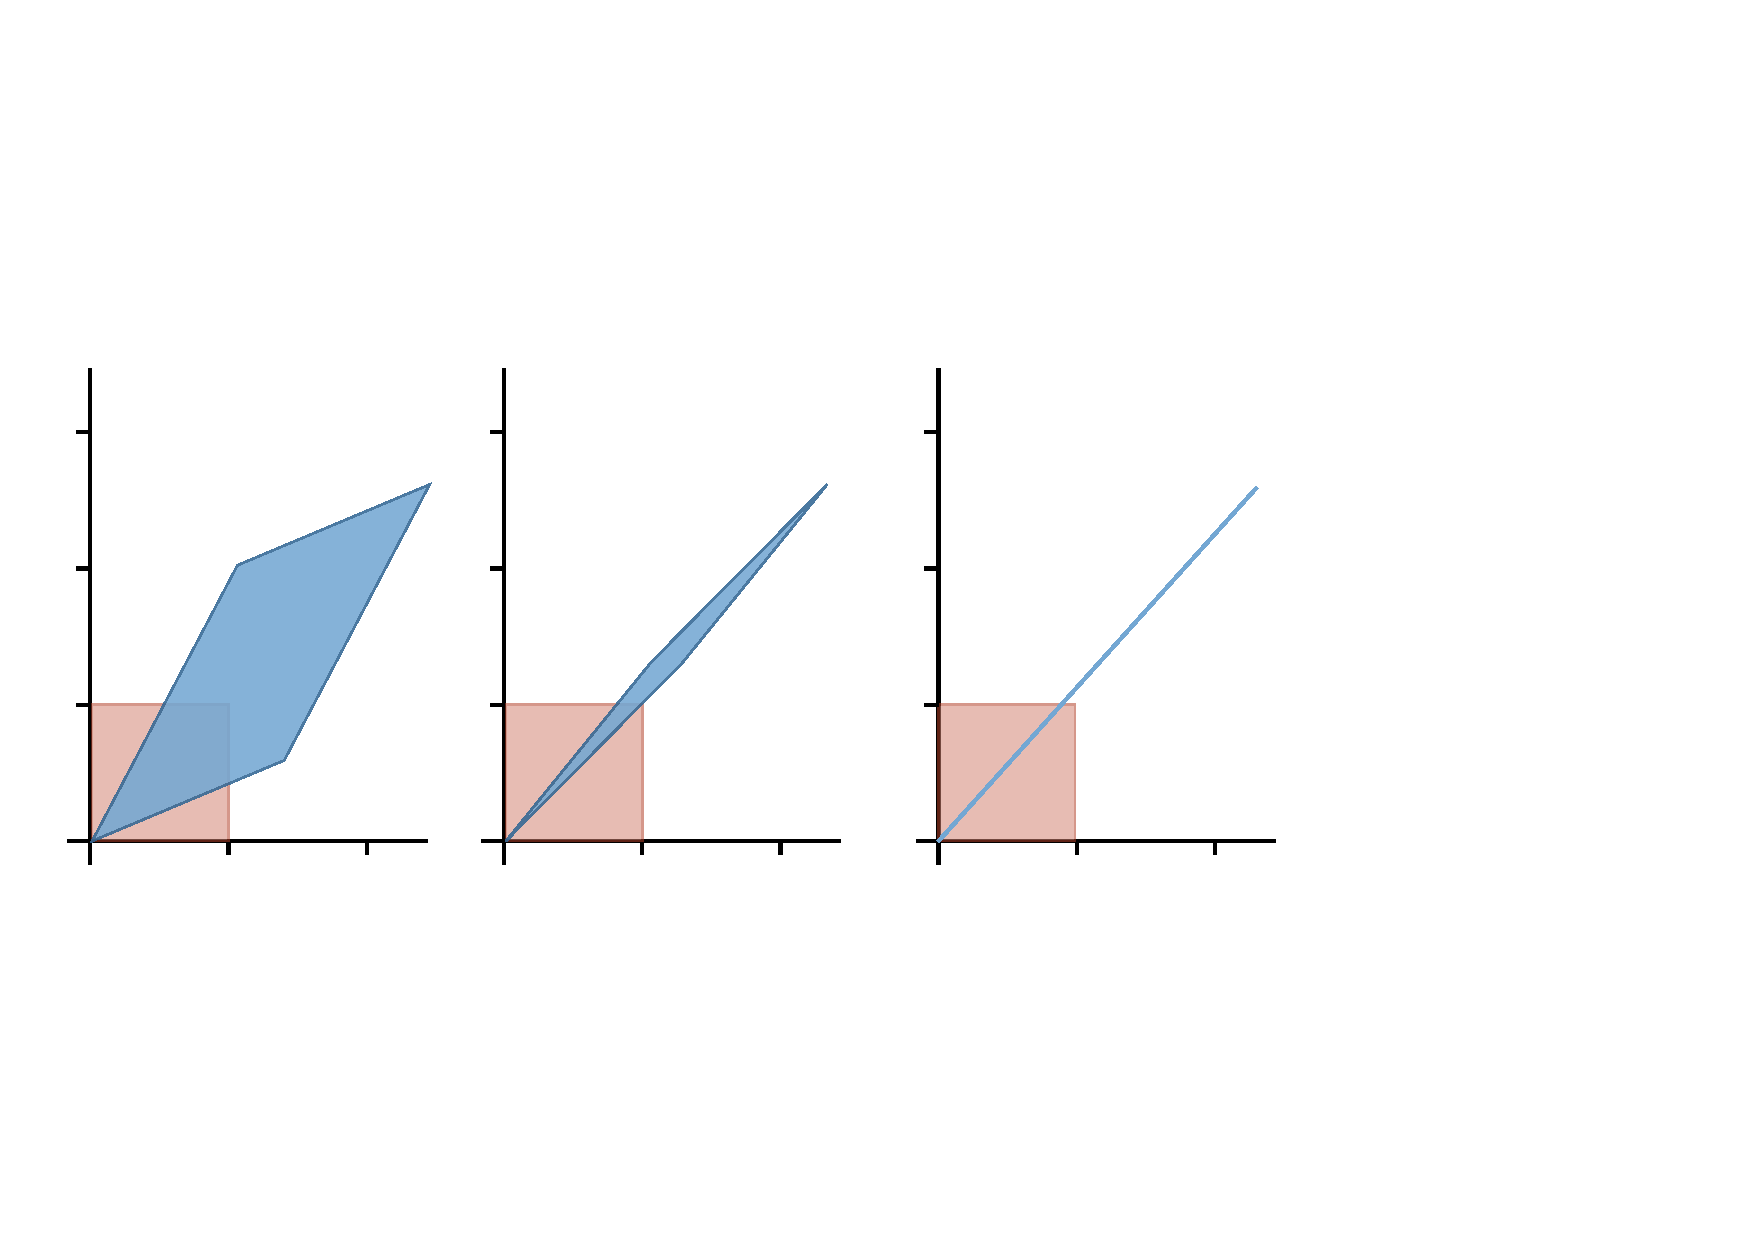
\includegraphics[width=1.2\textwidth]{./images/pca-3/invertible.pdf}
	}
	\caption*{Three transformations with increasingly small determinant. In the third, the unit square is squeezed into a line. Note that the two edges on the bottom left of the square are mapped to the same part of the line, so the transformation is not invertible. }
\end{figure}

%<figure class="narrow">
%<img src="/images/pca-3/invertible.svg" />
%<figcaption>Three transformations with increasingly small determinant. In the third, the unit square is squeezed into a line. Note that the two edges on the bottom left of the square are mapped to the same part of the line, so the transformation is not invertible. 
%</figcaption>
%</figure>

We don't need to know how to compute the determinant to know what its value is in this case. The unit square is mapped to a line segment, so its area goes from \(1\) to \(0\). This is how the determinant helps us to characterize invertible matrices: if the determinant is non-zero, the matrix is invertible, if the determinant is zero, the matrix is not invertible, or \emph{singular}. 

\index{Singular matrices}\index{Invertible matrices}

\subsection{Computing the \(2\times 2\) determinant}

Using this definition, it's pretty straightforward to work out what the formula is for the determinant of a matrix \(\bc{\mbA}\) that transforms a 2D space. We'll start by drawing a unit square, and labeling the four corners:

\begin{figure}[H]
	\centerline{
	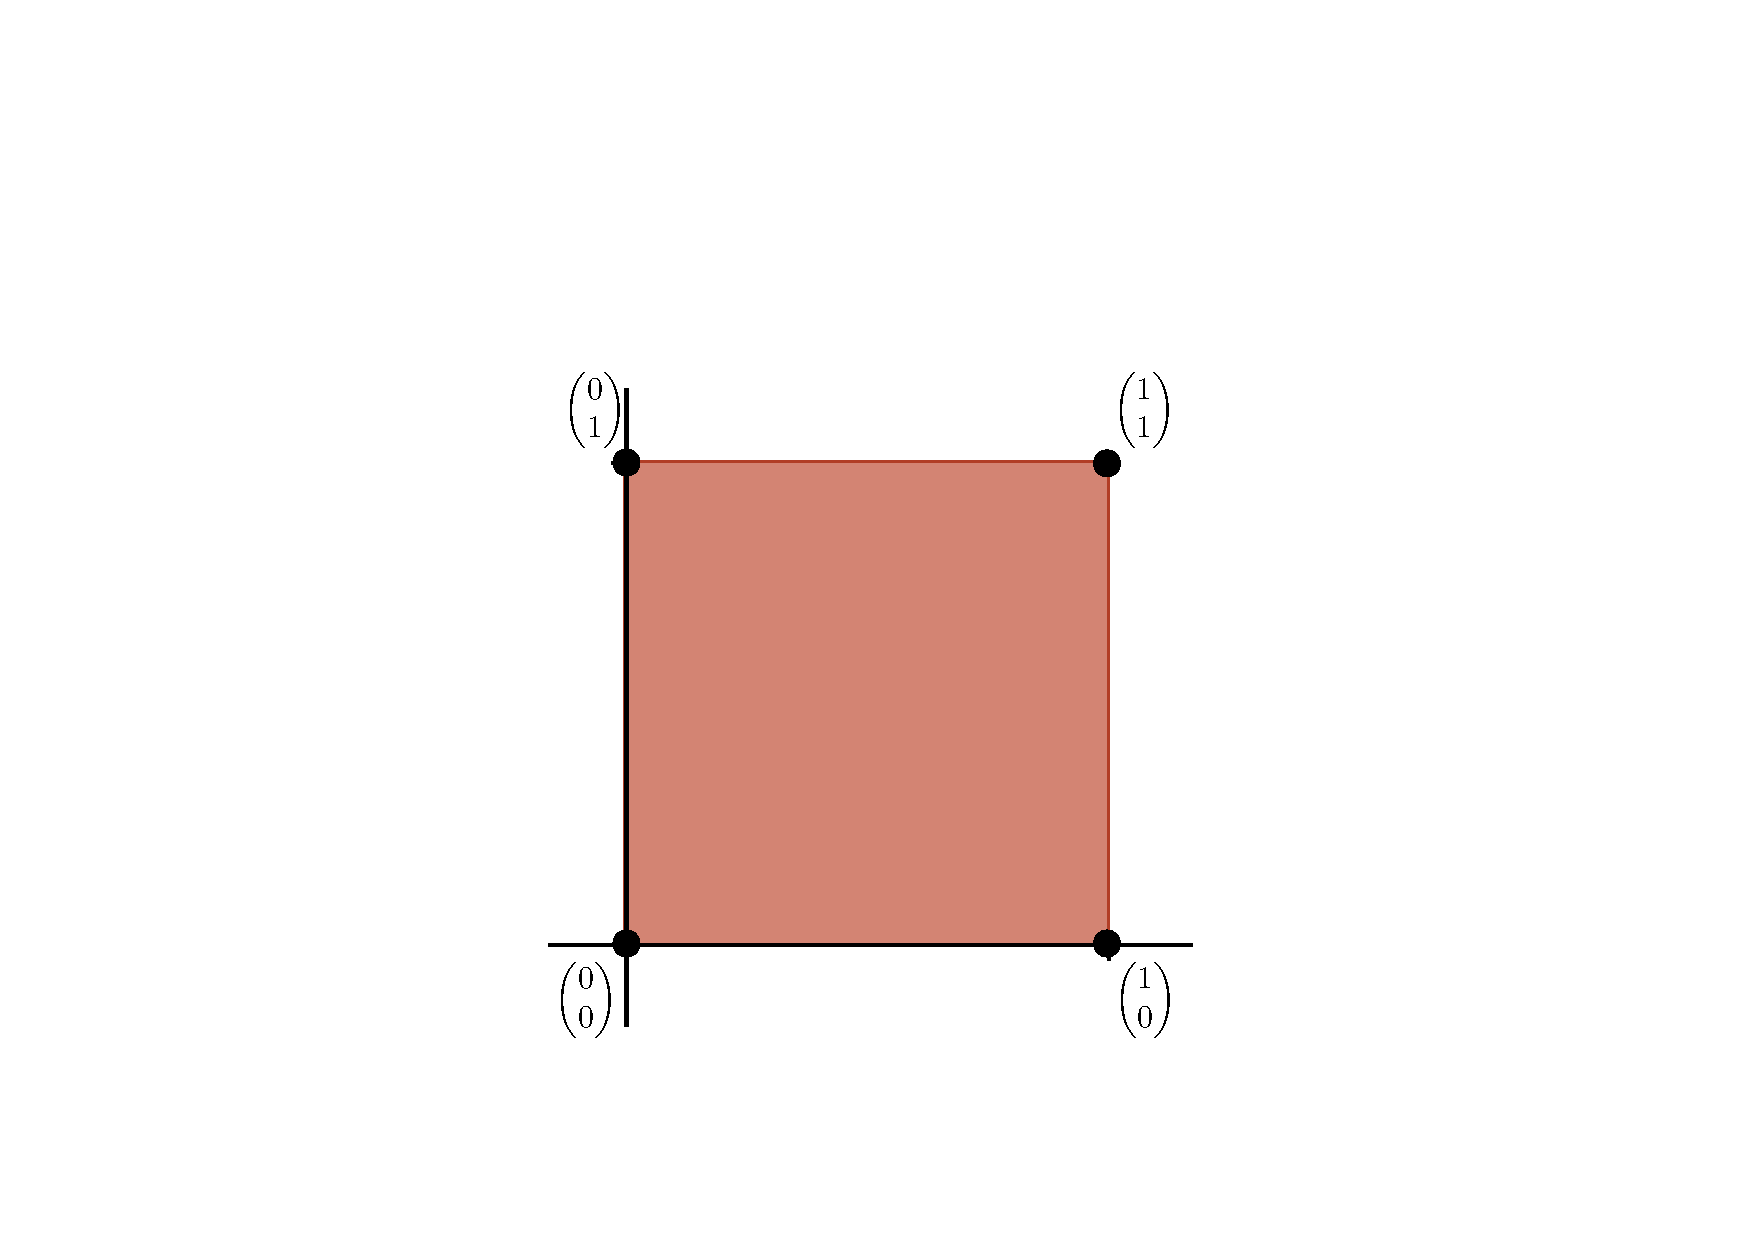
\includegraphics[width=0.4\textwidth]{./images/pca-3/corners.pdf}
	}
\end{figure}

%<figure class="fourth center">
%<img src="/images/pca-3/corners.svg" />
%</figure>

The corner points \((0,0)\), \((0,1)\) \((1,0)\) and \((1,1)\) can be transformed by multiplying them by \(\bc{\mbA}\). we know that under a linear operation like this, line segments stay line segments, so the four edges of the square are transformed to line segments, and the resulting figure between the four points must be a quadrilateral. We also know that \emph{parallelism is preserved}: two line segments that were parallel before the transformation are parallel after. Lastly, we know that the origin stays where it is, unless we apply a translation, so corner \((0, 0)\) is not affected by the transformation. All this means that the picture after the transformation will look something like this.

\begin{figure}[H]
	\centerline{
	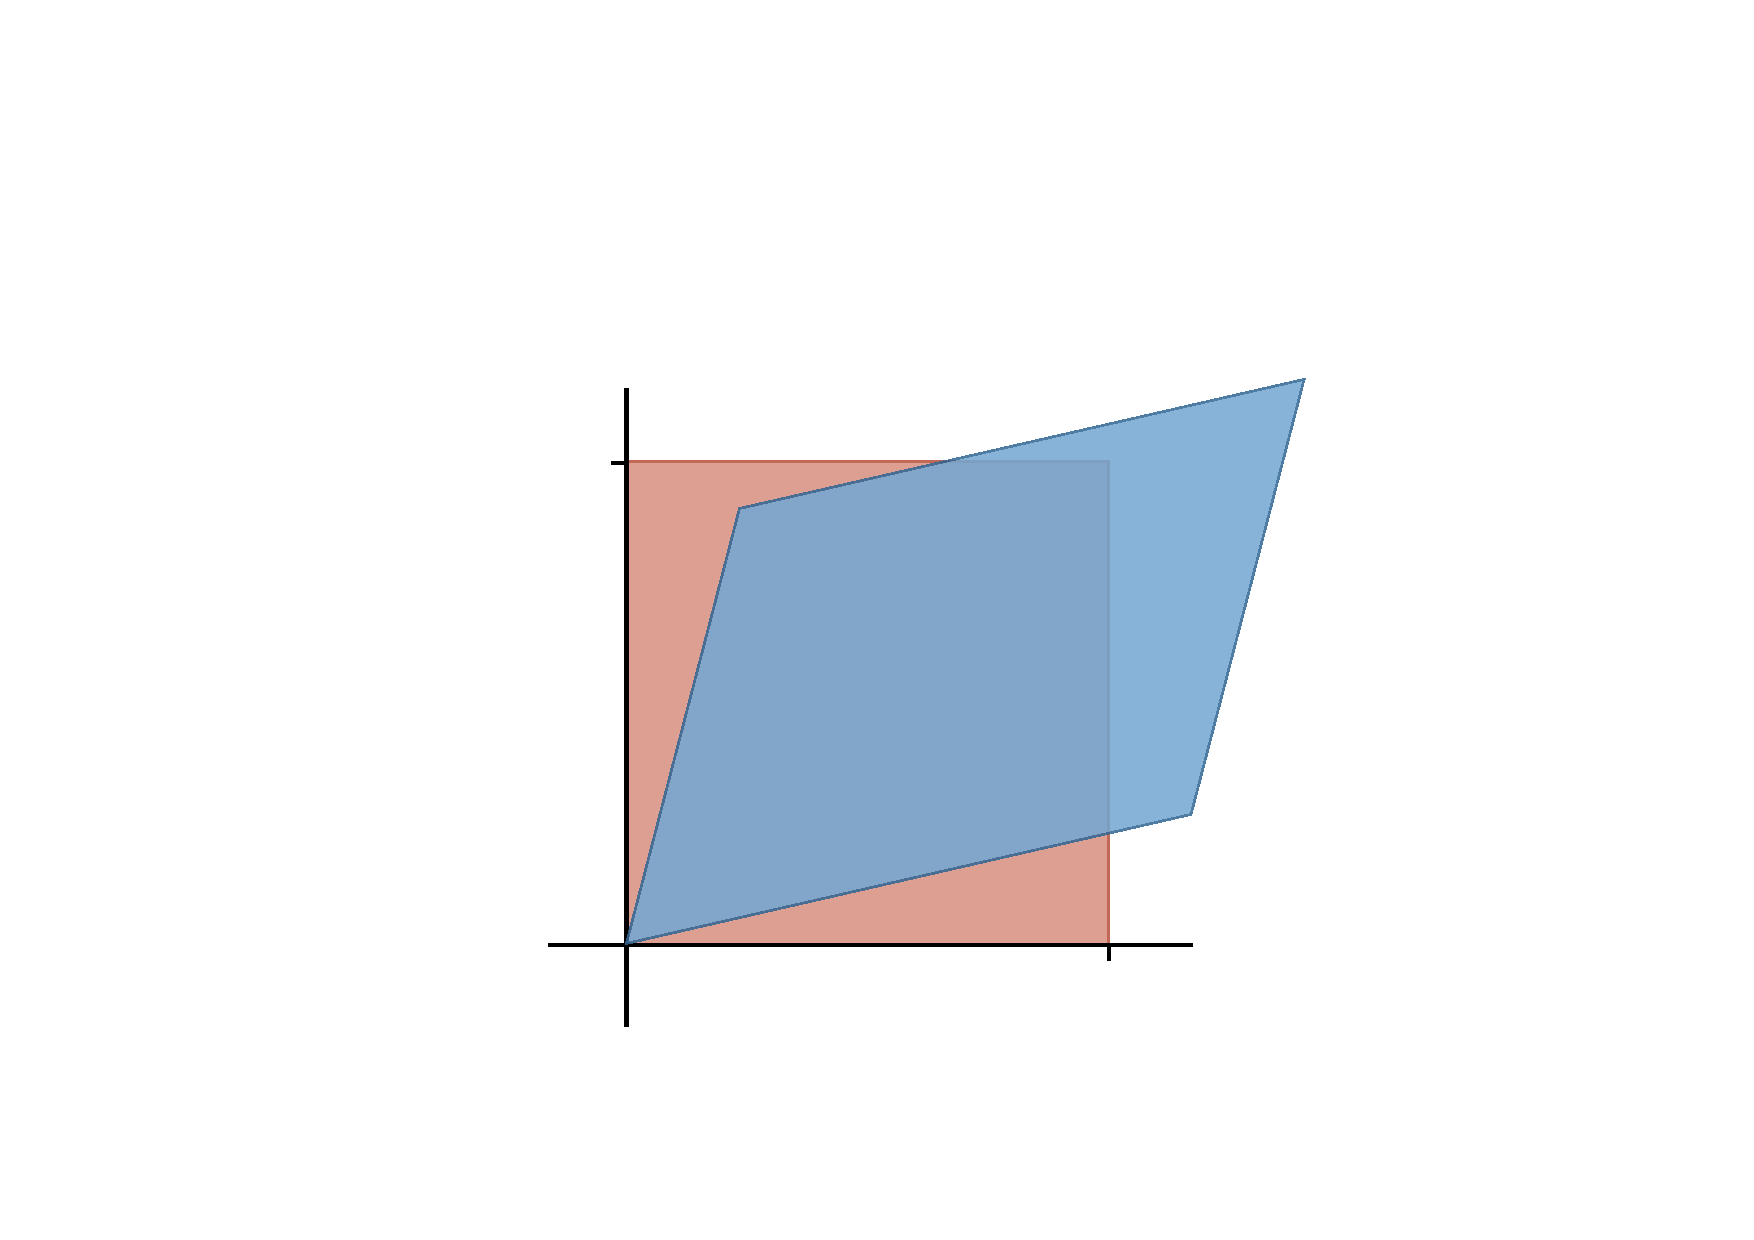
\includegraphics[width=0.6\textwidth]{./images/pca-3/pgram.pdf}
	}
\end{figure}
%<figure class="fourth center">
%<img src="/images/pca-3/pgram.svg" />
%</figure>

A parallelogram with one corner touching the origin. The determinant tells us the ratio between the area of \bc{the paralellogram} and \rc{the original square}. Since the original square has area \(1\), the area of the parallelogram is the determinant of \(\bc{\mbA}\). 

Working this out requires only a small amount of basic geometry. Here's the simplest way to do it.

We first name the four elements of our matrix:

\[
\bc{\mbA} = \begin{pmatrix} a & b \\ c & d \end{pmatrix}
\]

We can now name the four corners of our parallelogram in terms of these four scalars, by multiplying the corner points of the unit square by \(\bc{\mbA}\):

\[
\begin{matrix}
\times
& \begin{pmatrix}0\\ 0\end{pmatrix}
& \begin{pmatrix}1\\ 0\end{pmatrix} 
& \begin{pmatrix}0\\ 1\end{pmatrix} 
& \begin{pmatrix}1\\ 1\end{pmatrix} 
\\
\bc{\begin{pmatrix} a & b \\ c & d \end{pmatrix}}
& \begin{pmatrix}0\\ 0\end{pmatrix}
& \begin{pmatrix}a\\ c\end{pmatrix}
& \begin{pmatrix}b\\ d\end{pmatrix}
& \begin{pmatrix}a+b\\ c+d\end{pmatrix}
 \\
\end{matrix}
\]

This gives us the following picture.

\begin{figure}[H]
	\centerline{
	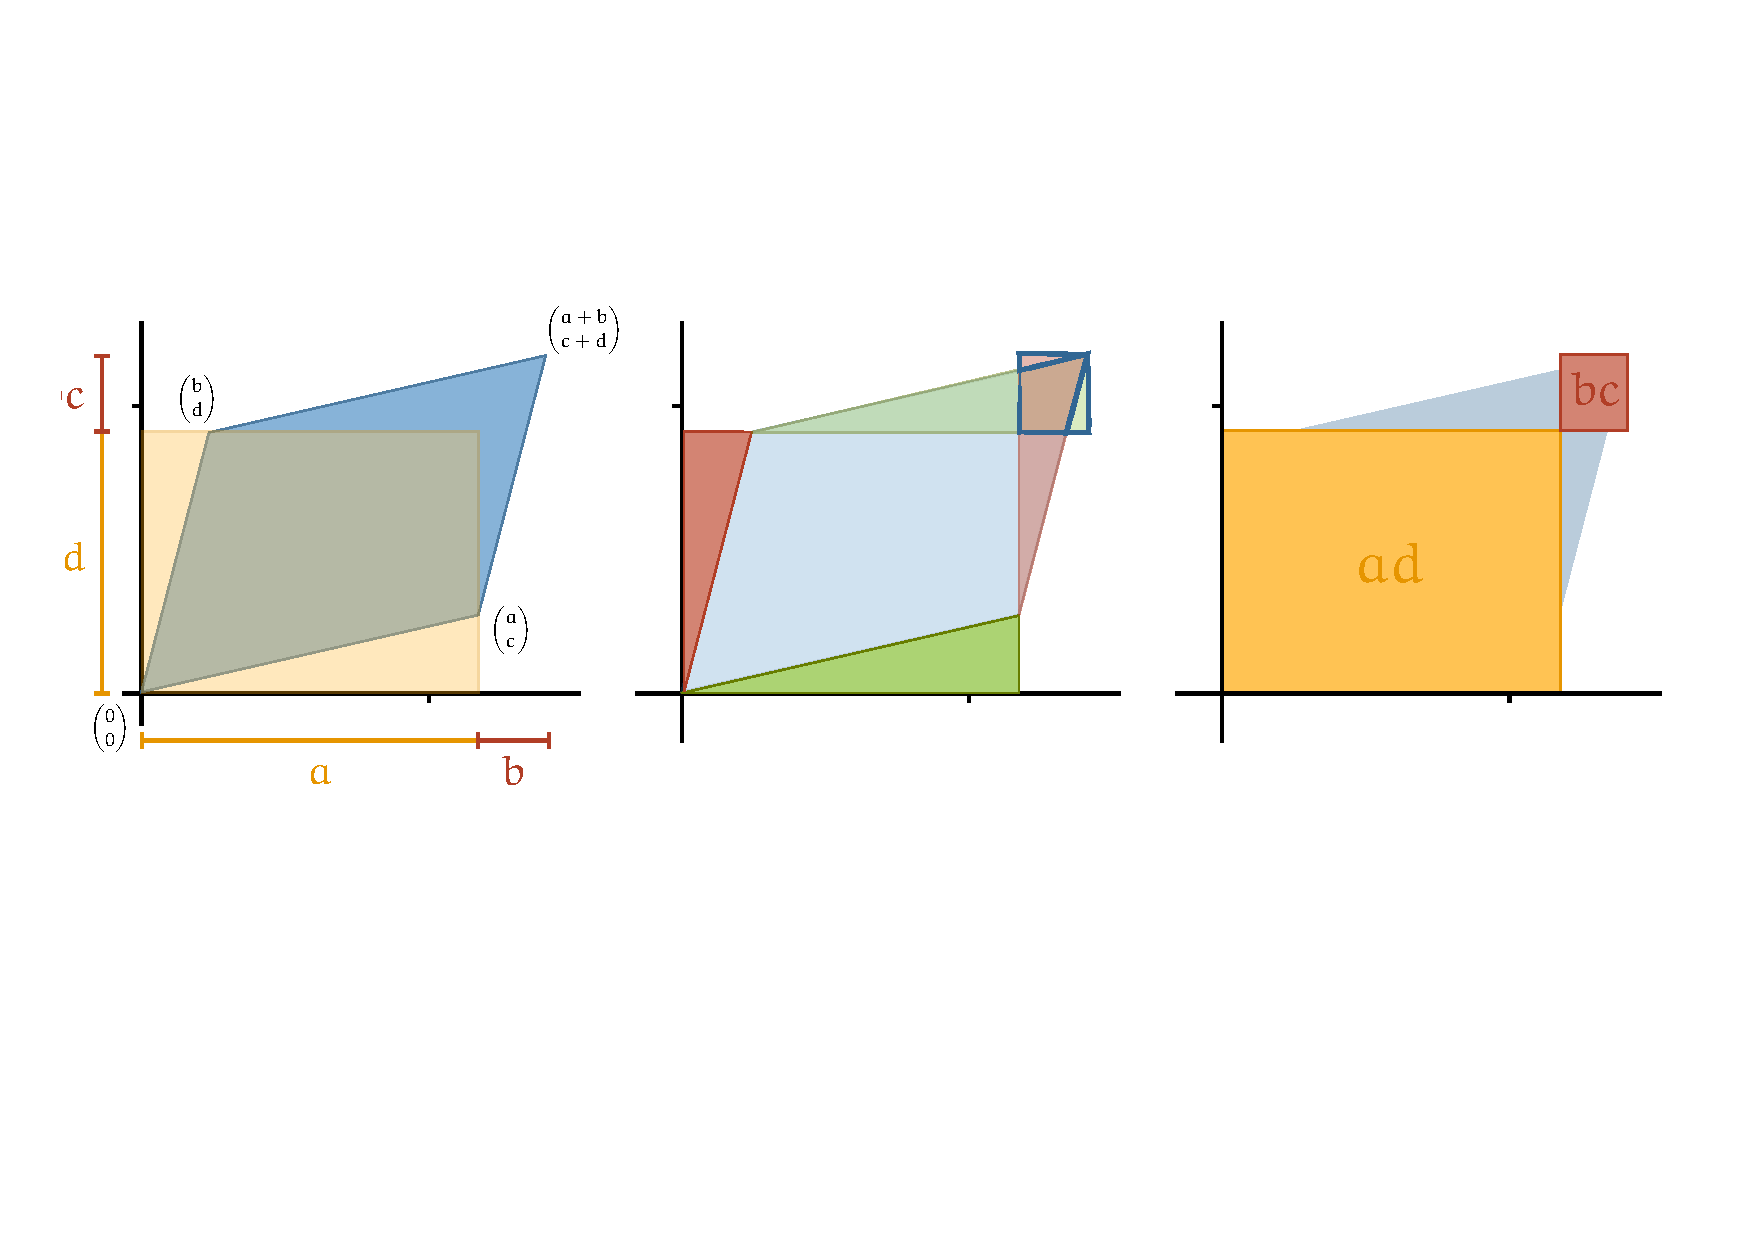
\includegraphics[width=1.3\textwidth]{./images/pca-3/geometric.pdf}
	}
\end{figure}
%<figure class="wide centering">
%<img src="/images/pca-3/geometric.svg" class="own-size"/>
%</figure>

Here we can see the area of the paralellogram clearly: there is one \oc{large rectangle} of area \(\oc{ad}\). To get from this area to the area of our parallelogram, we should subtract the area of the green triangle in the bottom, which is part of the rectangle but not the parallelogram. 

But then, there's a green triangle at the top, with the same size, which is (mostly) part of the parallelogram but not of the rectangle, so these cancel each other out. We follow the same logic for the red triangles.

Putting all this together, the rectangle with area \(\oc{ad}\) has the same area as the parallellogram, except that we are overcounting three elements (outlined in blue): the two small triangles in the box at the top, which are not part of the paralellogram, and the overlap between the green and the red triangles, which we've counted twice. These three overcounted elements  add up precisely to the box at the top-right, which has area \(\rc{bc}\). 

So, the area of the paralellogram, and therefore the determinant of the matrix \(\bc{\mbA}\) is \(\oc{ad} - \rc{bc}\). Or, in words: the determinant of a \(2 \times 2\) matrix is the diagonal product minus the antidiagonal product. 

%\begin{aside}
%If you don't trust such visual proofs, here it is algebraically:
%\begin{align*}
%\text{det}\;\bc{\mbA} + 2\left (\tfrac{1}{2}ac + \tfrac{1}{2}bd 2bc\right ) &= (a + b)(b + d)\\
%\text{det}\;\bc{\mbA} + \kc{ac} + \kc{bd} + 2bc &= \kc{ac} + ad + bc + \kc{bd}\\
%\text{det}\;\bc{\mbA} &= ad - bc
%\end{align*}
%\end{aside}

We will write the determinant of a matrix \(\bc{\mbA}\) with two vertical bars around the matrix. When we write out the values of the matrix explicitly, we will remove the matrix parentheses for clarity:

\[
|\bc{\mbA}| = \left |\, \begin{matrix} \oc{a} & \rc{b} \\ \rc{c} & \oc{d} \end{matrix} \;\right | = \oc{ad} - \rc{bc} \p
\]

\subsection{Negative determinants}

\index{Determinant!Negative-valued}

In the picture we drew to derive this, \(ad\) was bigger than \(bc\), so the determinant was positive. But this is not guaranteed. Look at the two column vectors of our matrix. If we flip them around then the determinant becomes:

\[
\left |\,\begin{matrix} \rc{b}  & \oc{a} \\ \oc{d} & \rc{c} \end{matrix}\; \right | = \rc{bc} - \oc{da} \p
\]

Assuming the values in the matrix are the same, this is the same quantity as before, but negative. Areas can't be negative, so how do we interpret this?

The magnitude remains the same, so the simplest solution is just to adjust our definitions: \emph{the absolute value} of \(|\bc{\mbA}|\) is the amount by which \(\bc{\mbA}\) inflates space.

However, in many situations, the idea of a ``negative area'' actually makes a lot of sense. Consider, for instance, this graph of the velocity of a train along a straight track from one station to another and back again:

\index{Negative area}\index{Signed area}

\begin{figure}[H]
	\centerline{
	\hspace{-0.9cm}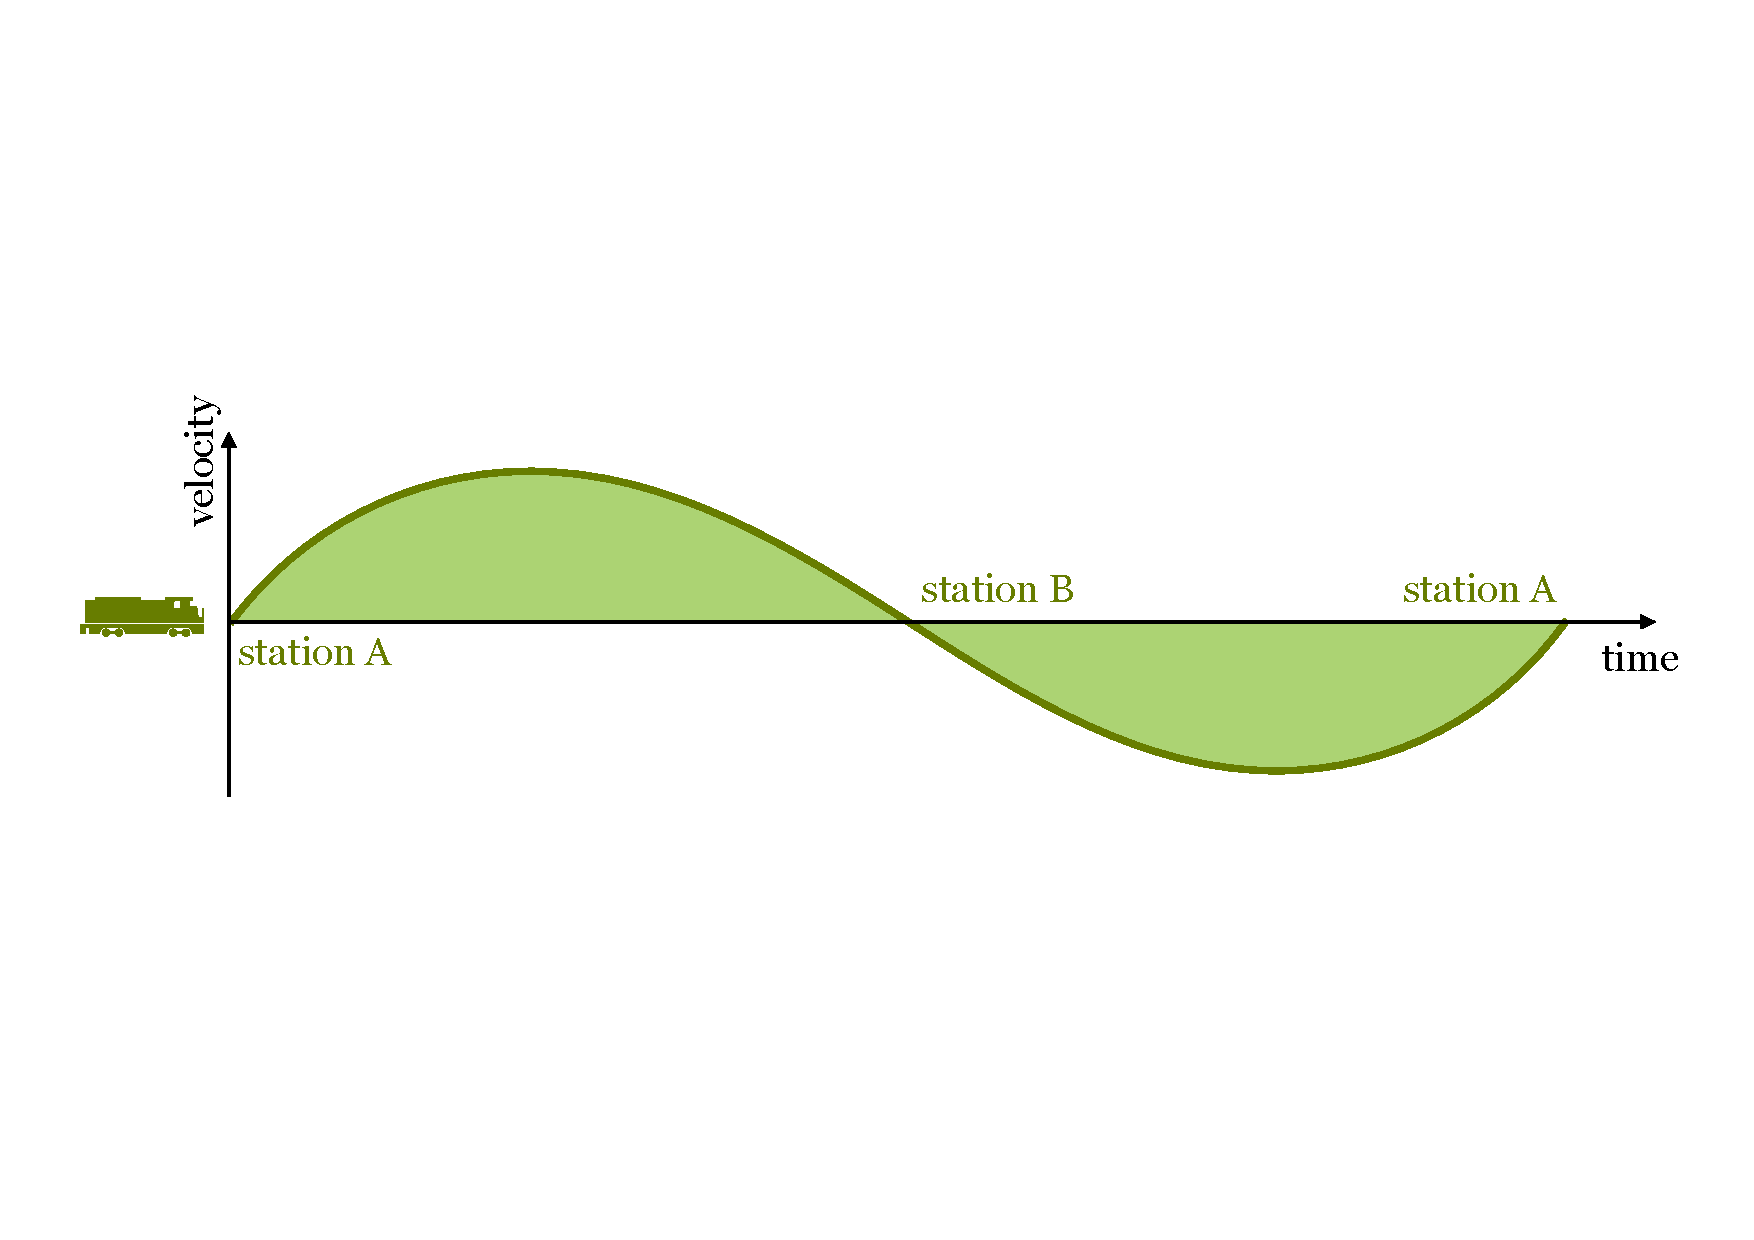
\includegraphics[width=1.1\textwidth]{./images/pca-3/train.pdf}
	}
\end{figure}
%<figure class="narrow">
%<img src="/images/pca-3/train.svg" />
%</figure>

Here, we've used a negative velocity to represent the train traveling backwards. If you've done some physics, then you'll know that the area under the speed curve represents distance traveled. Here we have two options: we can look at the absolute value of the area, and see that the train has, in total, travelled twice the distance between the stations. We can also take areas below the horizontal axis to be \emph{negative}. Then, their sum tells us that the total distance between the train's starting point and its final position is exactly zero.

All this is just to say, if you need positive areas, just take the magnitude of the determinant, but don't be too quick to throw away the sign. It may have some important meaning in your particular setting. For our purposes, we'll need these kinds of areas when we want to think about determinants for larger matrices.

We'll call this kind of positive or negative area a \emph{signed area}, or signed \emph{volume} in higher dimensions. You can think of the parallelogram as a piece of paper. If \(\bc{\mbA}\) stretches the paper, but doesn't flip it around, the singed area is positive. If the paper is flipped around, so that we see the reverse, the area is negative. If you flip the paper around twice, the sign becomes positive again.

\index{Signed volume}

\subsection{Towards \(n \times n\) determinants}

Let's think about what we'll need to generalize this idea to \(3 \times 3\) matrices and beyond, to general \(n \times n\) matrices. The basic intuition generalizes: we can start with a unit (hyper)cube in \(n\) dimensions. A square matrix transforms this into an analogue of a parallelogram, called a parallellotope. 

For a given dimensionality we can define a notion of \(n\)-volume. The 3-volume is simply the volume we already know. The \(n\)-volume of an n-dimensional ``brick'', the analogue of a rectangle, is the product of its extent in each direction: height times width times length and so on in all directions. This means that the unit hypercube, which has sides of length 1 in all directions, always has \(n\)-volume 1.

We will assume, by analogy with the \(2 \times 2\) case, that the determinant of an \(n \times n\) matrix \(\bc{\mbA}\) is the \(n\)-volume of the parallellotope that results when we transform the unit hypercube by \(\bc{\mbA}\). 

\begin{aside}Note that there are \(3 \times 3\) matrices that will flatten the unit cube into a parallelogram. In this case, we are \textbf{not} interested in the \emph{area} of the parallelogram as we were before. The matrix is \(3 \times 3\), so we care about the resulting \emph{volume}, which in such cases would be \(0\).
\end{aside}

We can generalize a few useful properties from the \(2 \times 2\) case. The columns of \(\bc{\mbA}\) are those vectors that describe the edges that touch the origin. We'll call these the \textbf{basis vectors} of the parallelogram/-tope.

\enlargethispage{3em}

\begin{figure}[H]
	\centerline{
	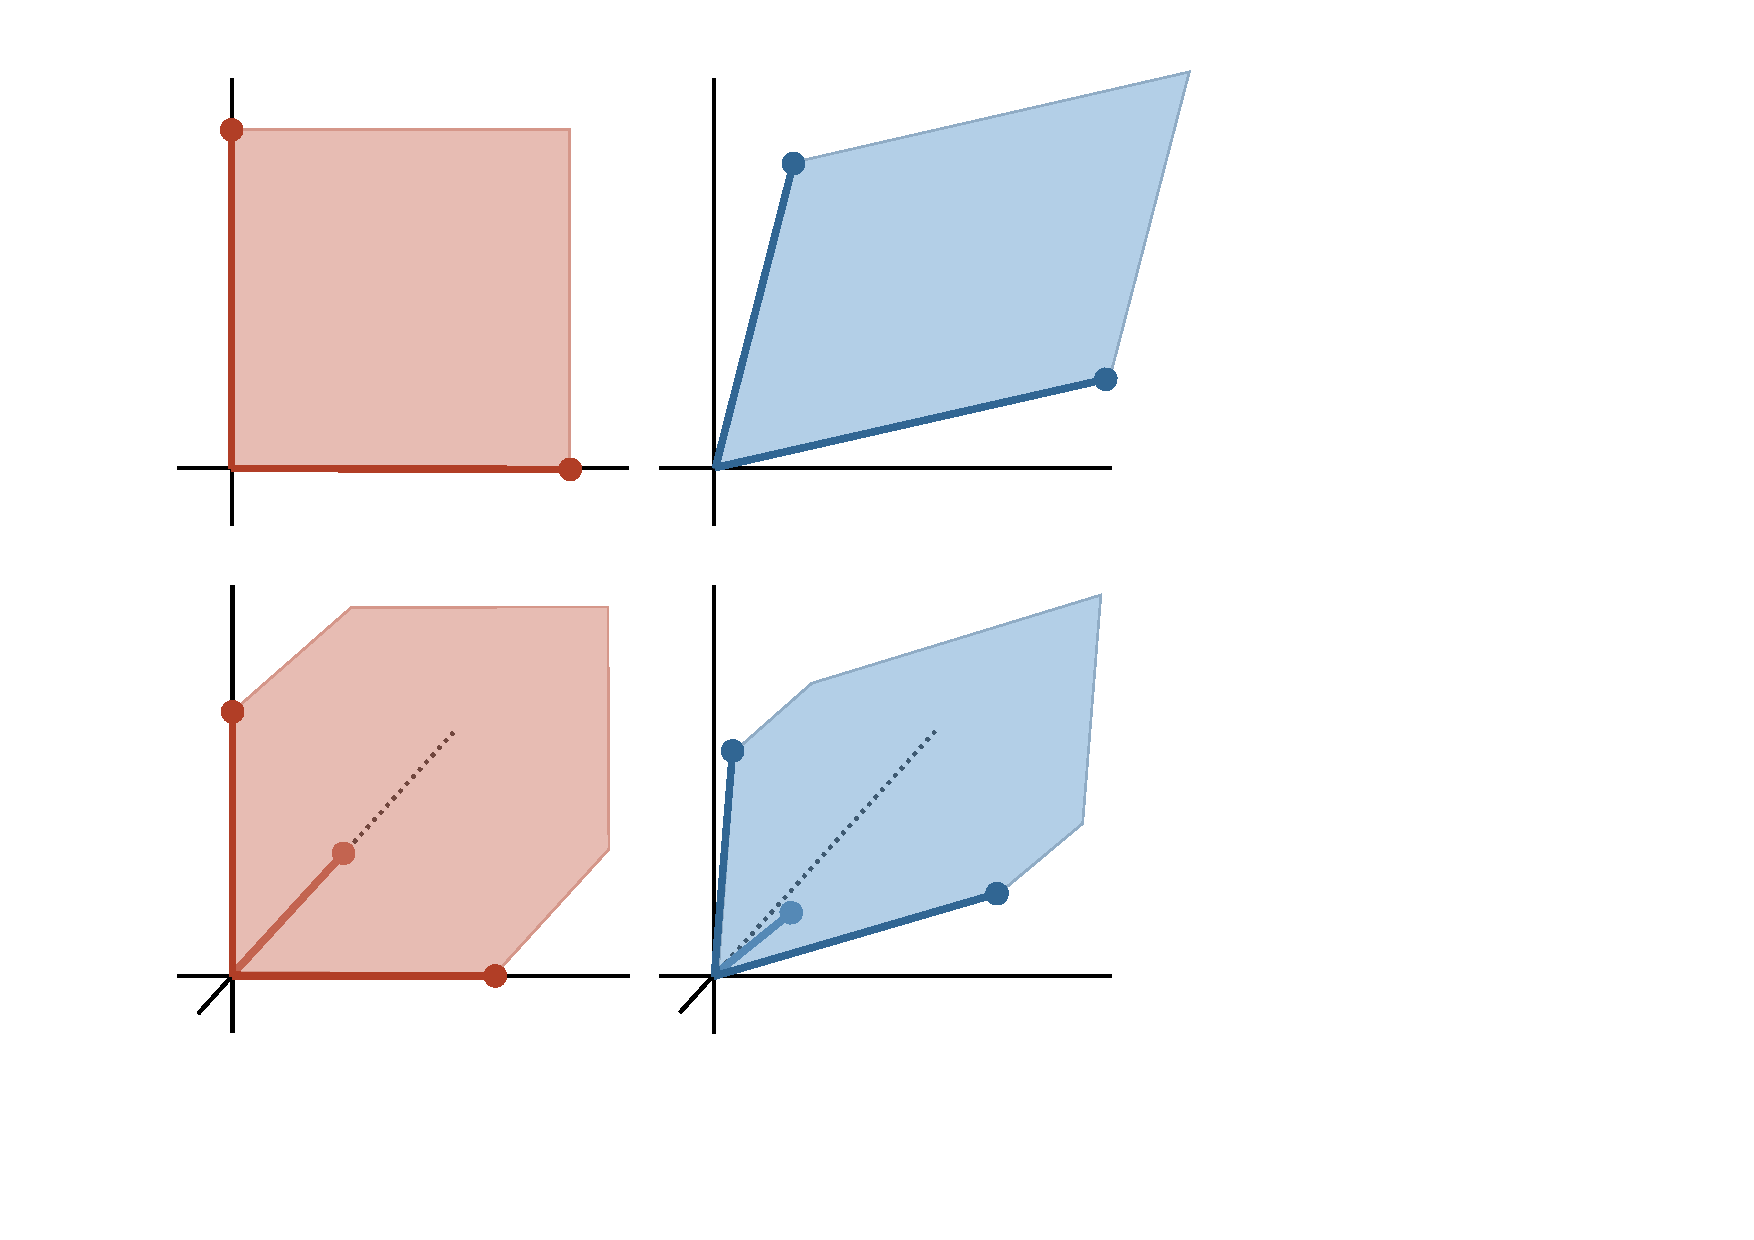
\includegraphics[width=0.8\textwidth]{./images/pca-3/basis-vectors.pdf}
	}
	\caption*{The edges of the \rc{unit cube} that touch the origin are the standard basis vectors. These are mapped to the edges of the \bc{parallelotope} that touch the origin. These are the column vectors of \(\bc{\mbA}\). We call these the \emph{basis vectors of the parallelotope}.
}
\end{figure}

%<figure class="narrow">
%<img src="/images/pca-3/basis-vectors.svg" />
%<figcaption>The edges of the <span class="rc">unit cube</span> that touch the origin are the standard basis vectors. These are mapped to the edges of the <span class="bc">parallelotope</span> that touch the origin. These are the column vectors of \(\bc{\A}\). We call these the <em>basis vectors of the parallelotope</em>.
%</figcaption>
%</figure>

The proof we gave for the \(2 \times 2\) determinant is very neat, but it isn't very easy to generalize to the \(n \times n\) case in an intuitive way.

%<!-- 
%<aside>It's not easy, but it is possible, if you use the idea that any two shapes that tile space with the same periodicity have the same volume. Here is <a href="https://math.stackexchange.com/a/2509560/24168">a StackExchange post that details this</a>. As neat as this is, it's a little involved for our purposes.
%</aside>
% -->

Instead, let's re-prove our result for the \(2 \times 2\) case in a way that's easier to generalize. We'll need to convince ourselves of three properties of the area of a parallellogram.

\begin{aside}These are not difficult to prove, but we'll focus here on the geometric intuition. If you want a more rigorous proof, it's easier to let this intuition go, and work purely symbolically.
\end{aside}

The \textbf{first property} we need is that if we move one of the sides of the parallelogram without changing its direction, the area of the parallellogram remains the same. This is easy to see visually.

\begin{figure}[H]
	\centerline{
	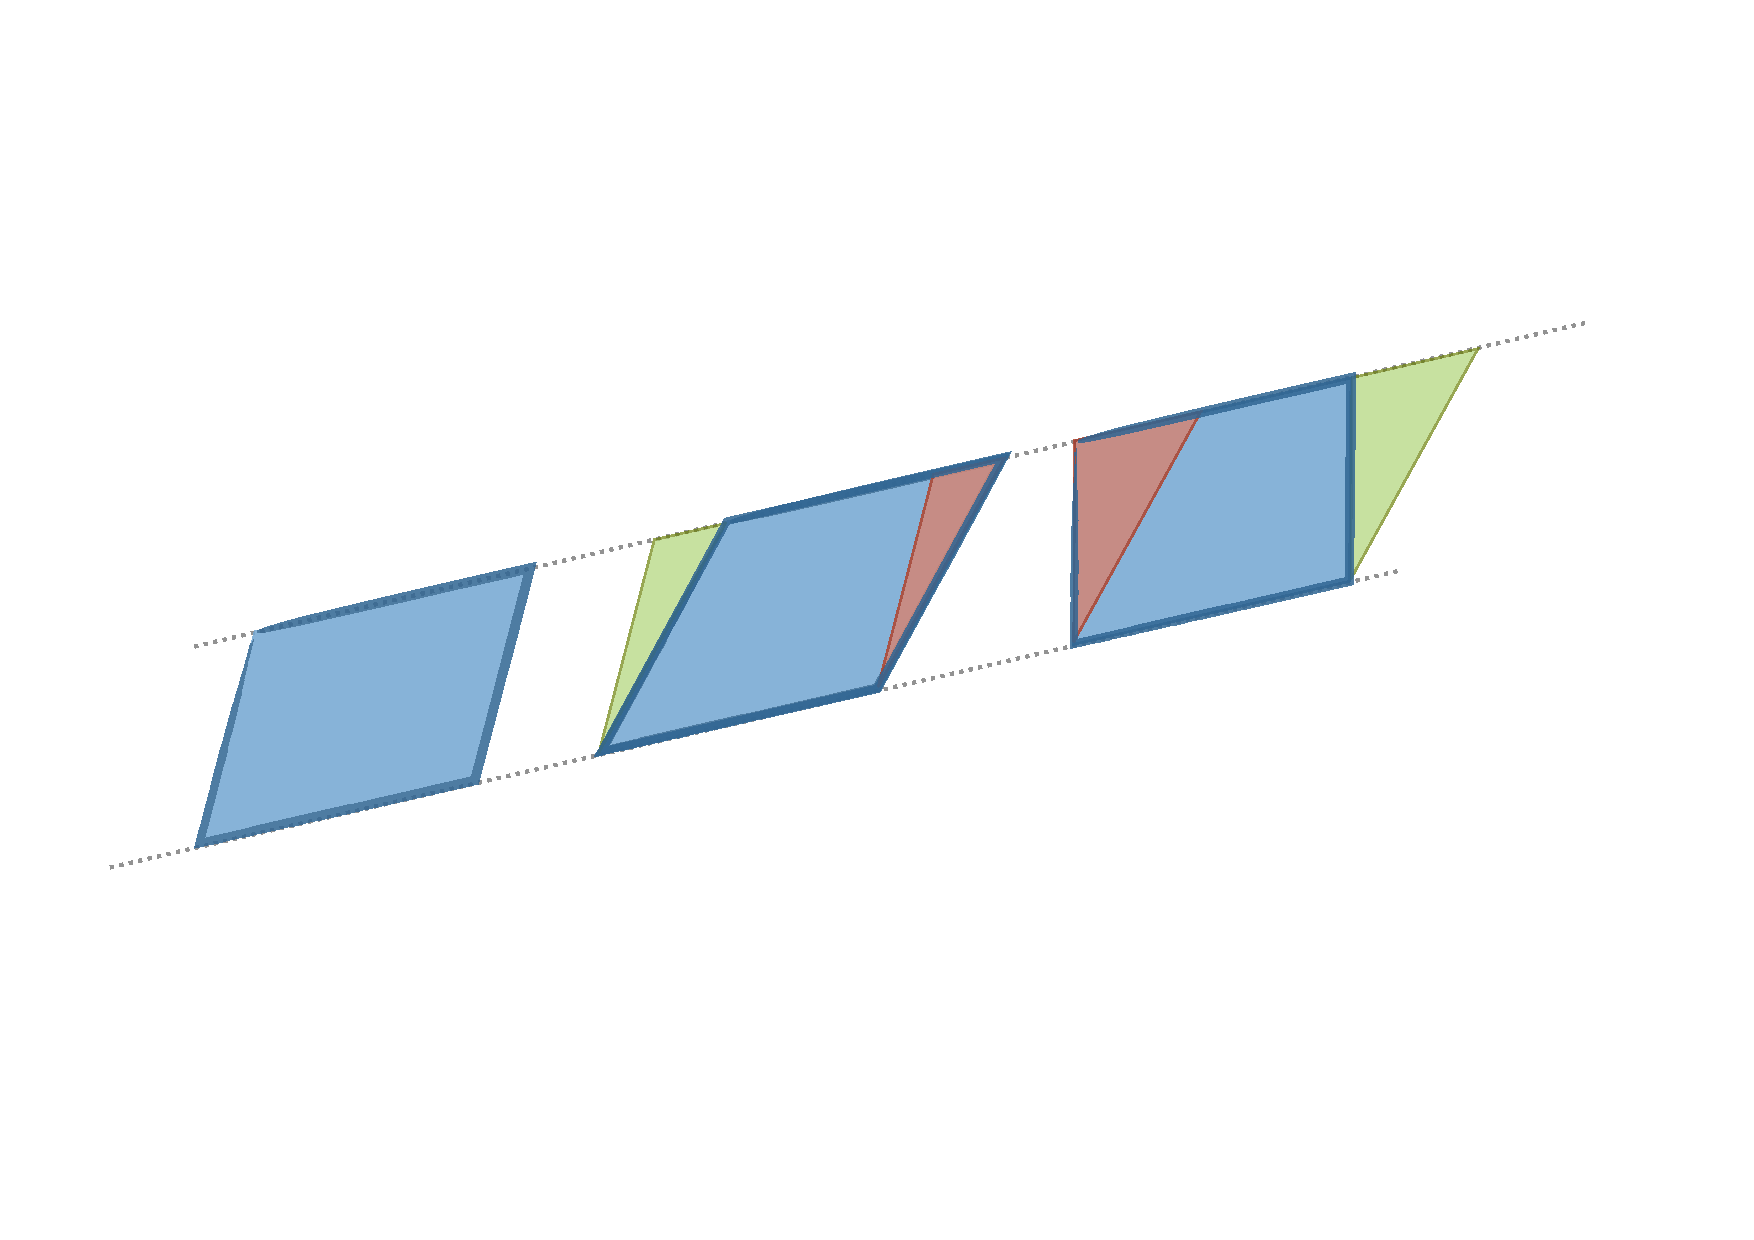
\includegraphics[width=1\textwidth]{./images/pca-3/skew.pdf}
	}
	\caption*{A skew transformation preserves the area of a parallelogram. This means we can align one of the edges with the axes without changing the area.
	}
\end{figure}

%<figure class="narrow">
%<img src="/images/pca-3/skew.svg" />
%<figcaption>A skew transformation preserves the area of a parallelogram. This means we can align one of the edges with the axes without changing the area.
%</figcaption>
%</figure>

Note that shifting one of the sides always \rc{adds a triangle} to the parallellogram and \gc{takes away} a triangle of the same size, so the total stays the same. The last example is particularly relevant: we can shift the parallelogram so that one of its edges is aligned with one of the axes. If we do this twice, we'll have a \emph{rectangle} with an area equal to that of the original parallellogram.

\enlargethispage{2em}

What does this look like in the original matrix? Remember that the columns of the matrix are the two edges of the parallelogram that touch the origin. Shifting one of them in this way is equivalent to adding or subtracting a small multiple of the other to it.

\begin{figure}[H]
	\centerline{
	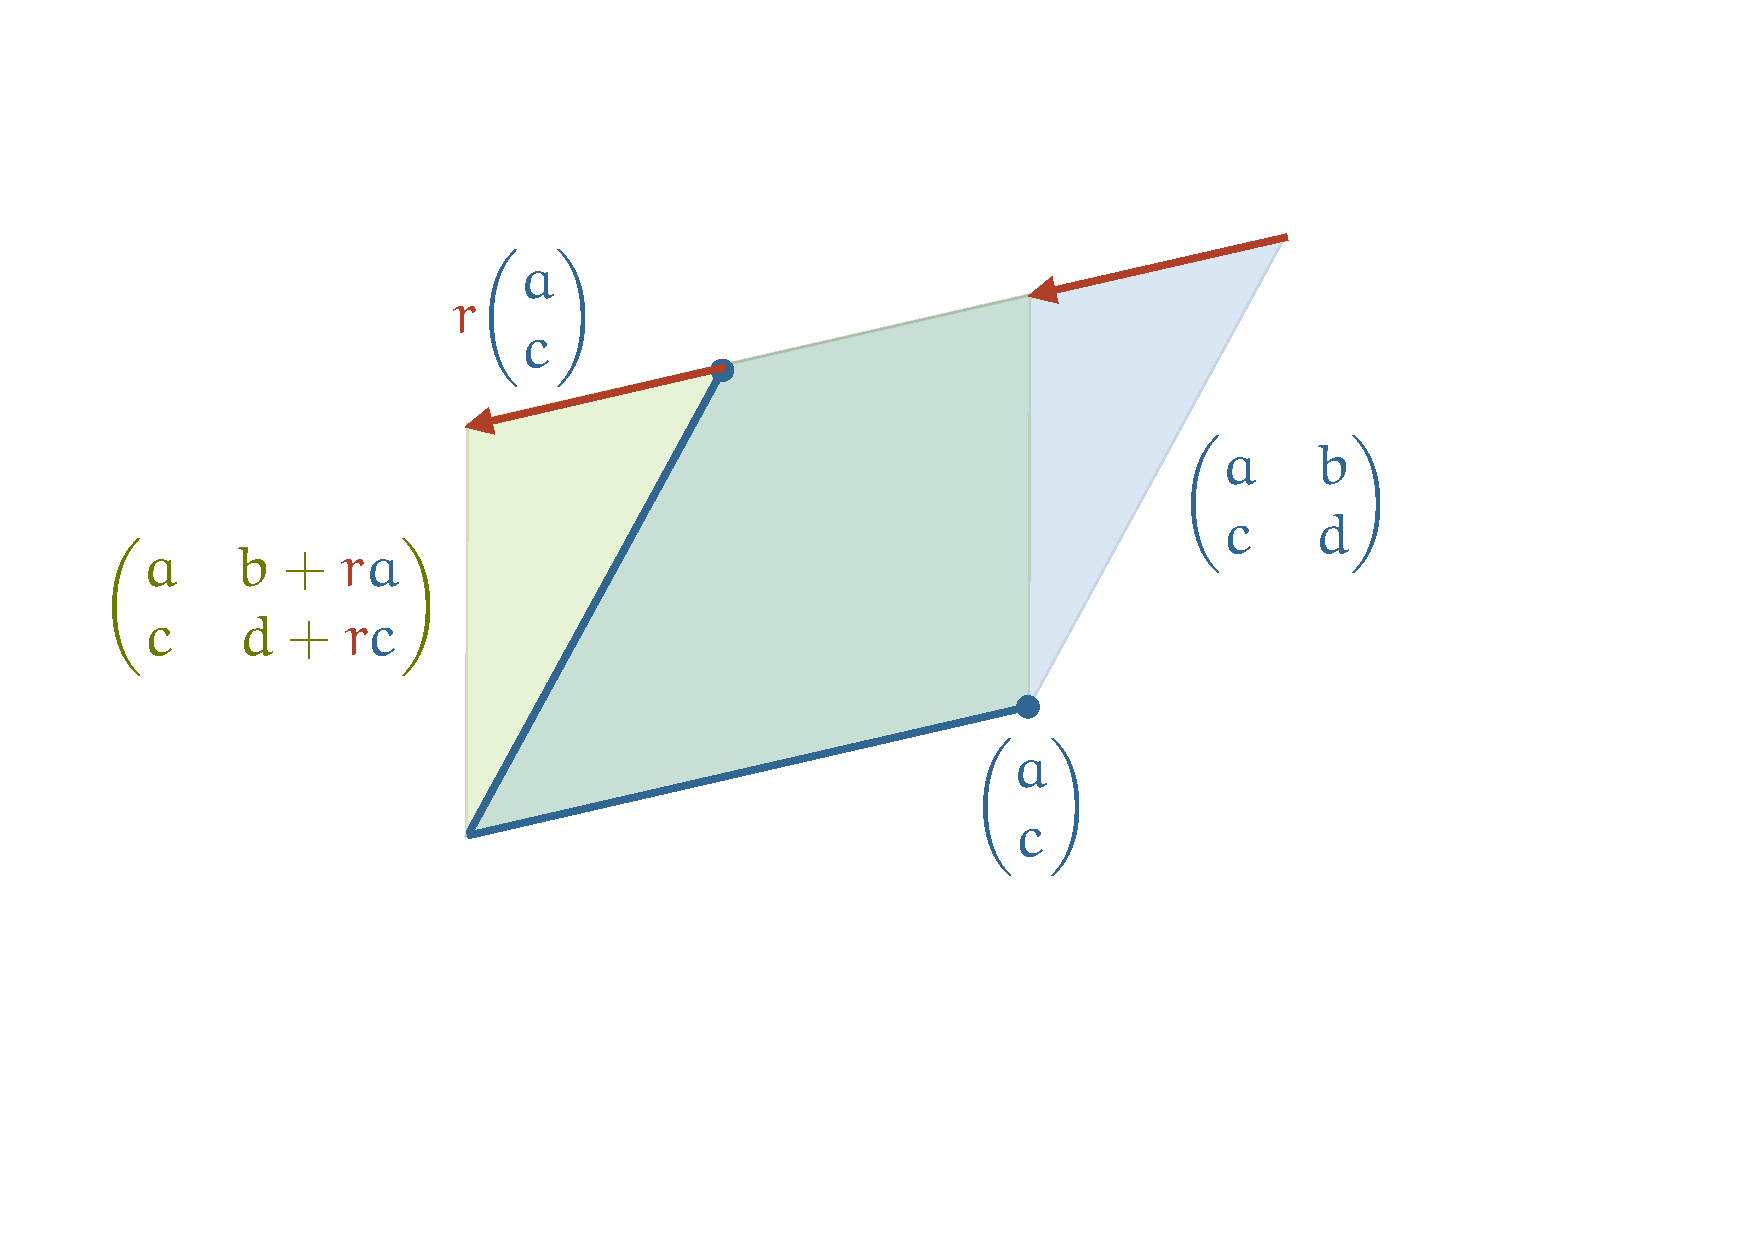
\includegraphics[width=1\textwidth]{./images/pca-3/align.pdf}
	}
	\caption*{To axis-align a parallellogram defined by a matrix, we take one of the columns, and add or subtract some multiple of the other column.
	}
\end{figure}

%<figure class="narrow">
%<img src="/images/pca-3/align.svg" />
%<figcaption>To axis-align a parallellogram defined by a matrix, we take one of the columns, and add or subtract some multiple of the other column.
%</figcaption>
%</figure>

That is, if we take one of the columns of \(\bc{\mbA}\), multiply it by any \rc{non-zero scalar}, and add it to another column, the area of the resulting parallelogram is unchanged. If we name the column vectors \(\bc{\mbv}\) and \(\bc{\mbw}\), and write \(|\,\bc{\mbv}, \bc{\mbw}\,|\) for the determinant of the matrix with these column vectors, then we have

\[
|\,\bc{\mbv}, \bc{\mbw}\,| = |\,\bc{\mbv} + \rc{r}\bc{\mbw}, \bc{\mbw}\,| \;\;\text{for any nonzero \(\rc{r}\).}
\]

This kind of transformation is called a skew or a shear, so we'll call this property \textbf{skew invariance}: the area of a parallelogram is skew invariant. 

\index{Skew transformation}\index{Shear transformation}\index{Skew invariance|textbf}

The \textbf{second property} we need, is that if we take one of the column vectors of the matrix, say \(\bc{\mbv}\), and write it as the sum of two other vectors \(\bc{\mbv} = \oc{\mbv}^1 + \oc{\mbv}^2\), then the area of the paralellogram made by basis vectors \(\bc{\mbv}, \bc{\mbw}\) is the sum of the area of the two smaller parallelograms with basis vectors \(\oc{\mbv}^1, \bc{\mbw}\) and \(\oc{\mbv}^2, \bc{\mbw}\) respectively.

This is easy enough to see if \(\oc{\mbv}^1\) and \(\oc{\mbv}^2\) point in the same direction. Then the two smaller parallelograms together simply combine to form the larger one.

If they don't point in the same direction, we can skew them until they do. Since we've already shown that the area is skew invariant, none of this changes the area of the paralellogram.

\begin{figure}[H]
	\centerline{
	\hspace{1em}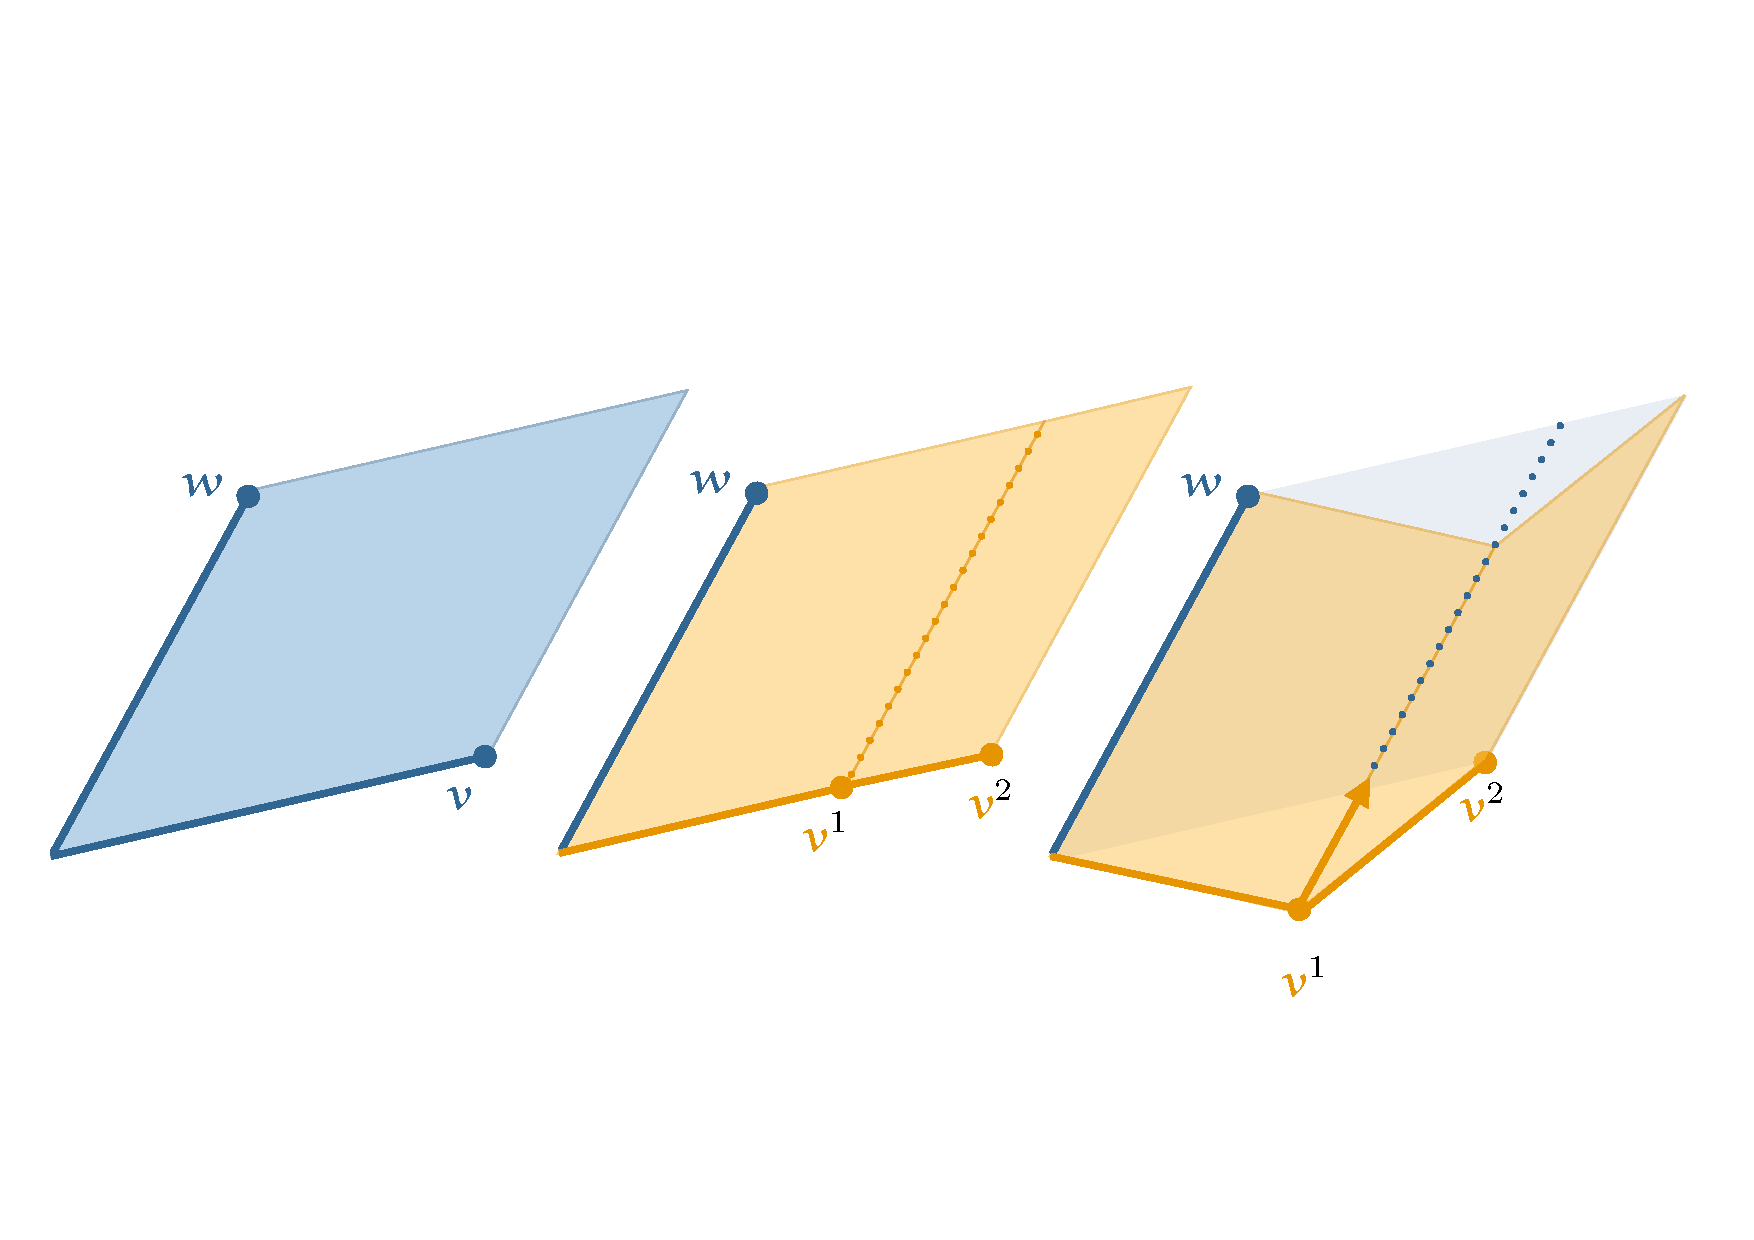
\includegraphics[width=1.2\textwidth]{./images/pca-3/sum.pdf}
	}
	\caption*{If we break one of the basis vectors into the sum of two other vectors, the original area is the sum of the two parts. This is easy to see if the sub-vectors point in the same direction as the original. If they don't, we simply skew them until they do.
	}
\end{figure}

%<figure class="narrow">
%<img src="/images/pca-3/sum.svg" />
%<figcaption>If we break one of the basis vectors into the sum of two other vectors, the original area is the sum of the two parts. This is easy to see if the sub-vectors point in the same direction as the original. If they don't, we simply skew them until they do.
%</figcaption>
%</figure>

Symbolically, this means that if we break one of the vectors in a matrix into a sum of two other vectors, then the determinant distributes over that sum:

\[
|\;\oc{\mbv}^1 + \oc{\mbv}^2, \bc{\mbw}\;| = |\;\oc{\mbv}^1, \bc{\mbw}\;| + |\;\oc{\mbv}^2, \bc{\mbw}\;| \p
\]

We won't need it here, but we can also show that multiplying one of the vectors by some scalar scales the determinant by the same value. These two properties together are called \textbf{multilinearity}: the area of a paralellogram is a multilinear function of the basis vectors. It's a linear function of one of its arguments if we keep the others fixed.

\index{Multilinearity|textbf}

We need \textbf{one more property}: if we start with a parallelogram with basis vectors \(\bc{\mbv}, \lbc{\mbw}\), and we flip around the vectors, \(\lbc{\mbw}, \bc{\mbv}\), what happens to the area? If we look at the picture of the parallellogram, at first, it's difficult to see that anything changes at all. The two basis vectors are still the same. To see what happens, we need to look at the operation of the matrix with these vectors as its columns. 

The matrix with columns \(\bc{\mbv}, \lbc{\mbw}\) maps the horizontal unit vector \(\mbe_h\) to \(\bc{\mbv}\), and the vertical unit vector \(\mbe_h\) to \(\lbc{\mbw}\). For the matrix with the columns swapped, we reverse this mapping. We get the same, parallelogram, but it's as if we've turned it over. Since the unit square has positive area, the flipped-over paralellogram has negative area.

\begin{figure}[H]
	\centerline{
	\hspace{0.5em}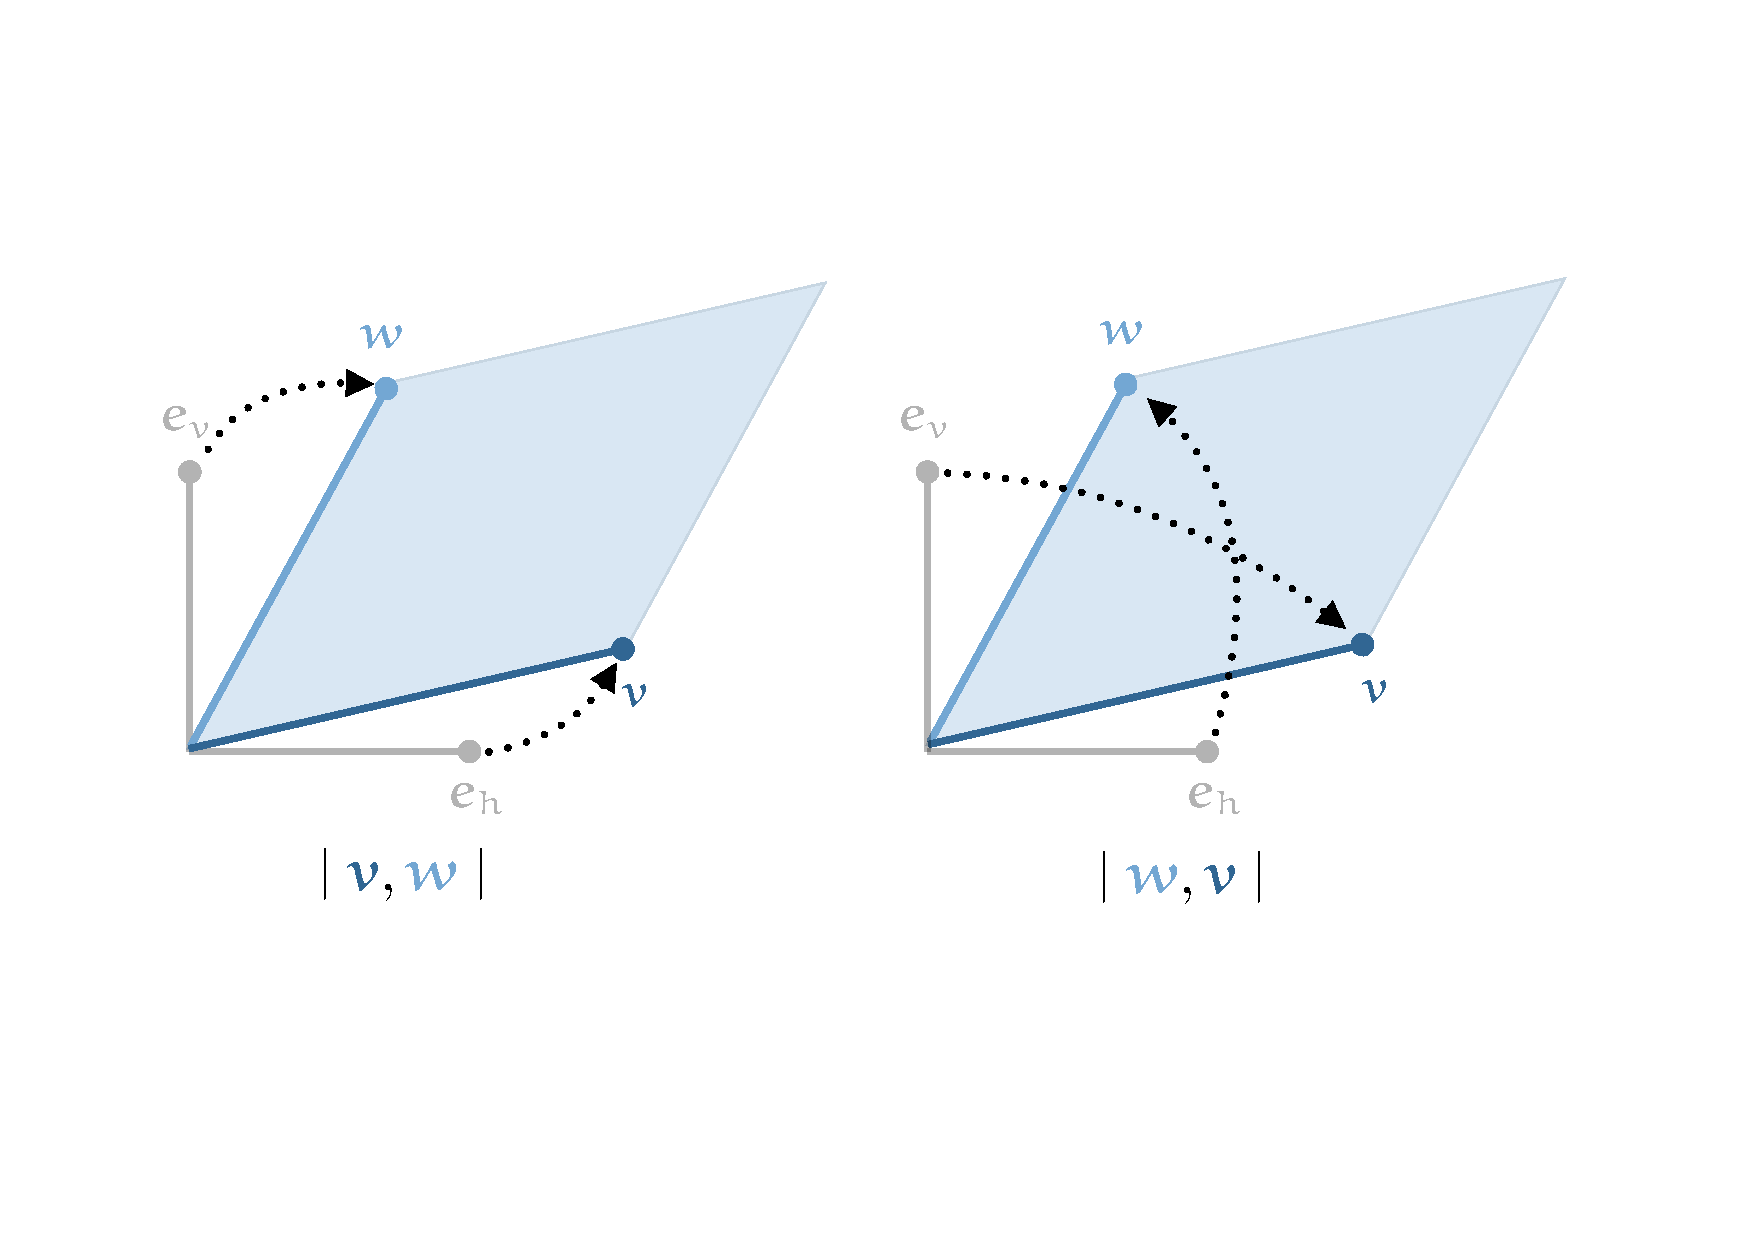
\includegraphics[width=1\textwidth]{./images/pca-3/alternativity.pdf}
	}
	\caption*{Swapping the columns of a matrix swaps the basis vectors of the paralellogram, turning a positive area into a negative area.
	}
\end{figure}

%<figure class="narrow">
%<img src="/images/pca-3/alternativity.svg" />
%<figcaption>Swapping the columns of a matrix swaps the basis vectors of the paralellogram, turning a positive area into a negative area.
%</figcaption>
%</figure>

Put simply, swapping basis vectors around maintains the magnitude of the area of a parallellogram, but changes the signs.

\[
|\;\bc{\mbv}, \lbc{\mbw}\;| = - |\;\lbc{\mbw}, \bc{\mbv}\;| \p
\]

We call this property \textbf{alternativity}. As in, the area of a parallelogram is and alternating function of its basis vectors. 

\index{Alternativity}

With these three properties: skew invariance, multilinearity and alternativity, we can work out our new proof of the determinant formula. First, using multilinearity, we write the first column of matrix \(\bc{\mbA}\) as the sum of two vectors:

\[
\left |\,\begin{matrix} ~a & b \\ c & d\end{matrix}\; \right | = \left | \,\begin{matrix} ~a & b \\ \kc{0} & d\end{matrix}\; \right | + \left | \,\begin{matrix} ~\kc{0} & b \\ c & d\end{matrix}\; \right | \p
\]

We'll call this kind of vector, where only one element is non-zero, a \textbf{simple vector}. Here's a visualization of that step.

\index{Simple vector}\index{Vector!Simple}

\begin{figure}[H]
	\centerline{
		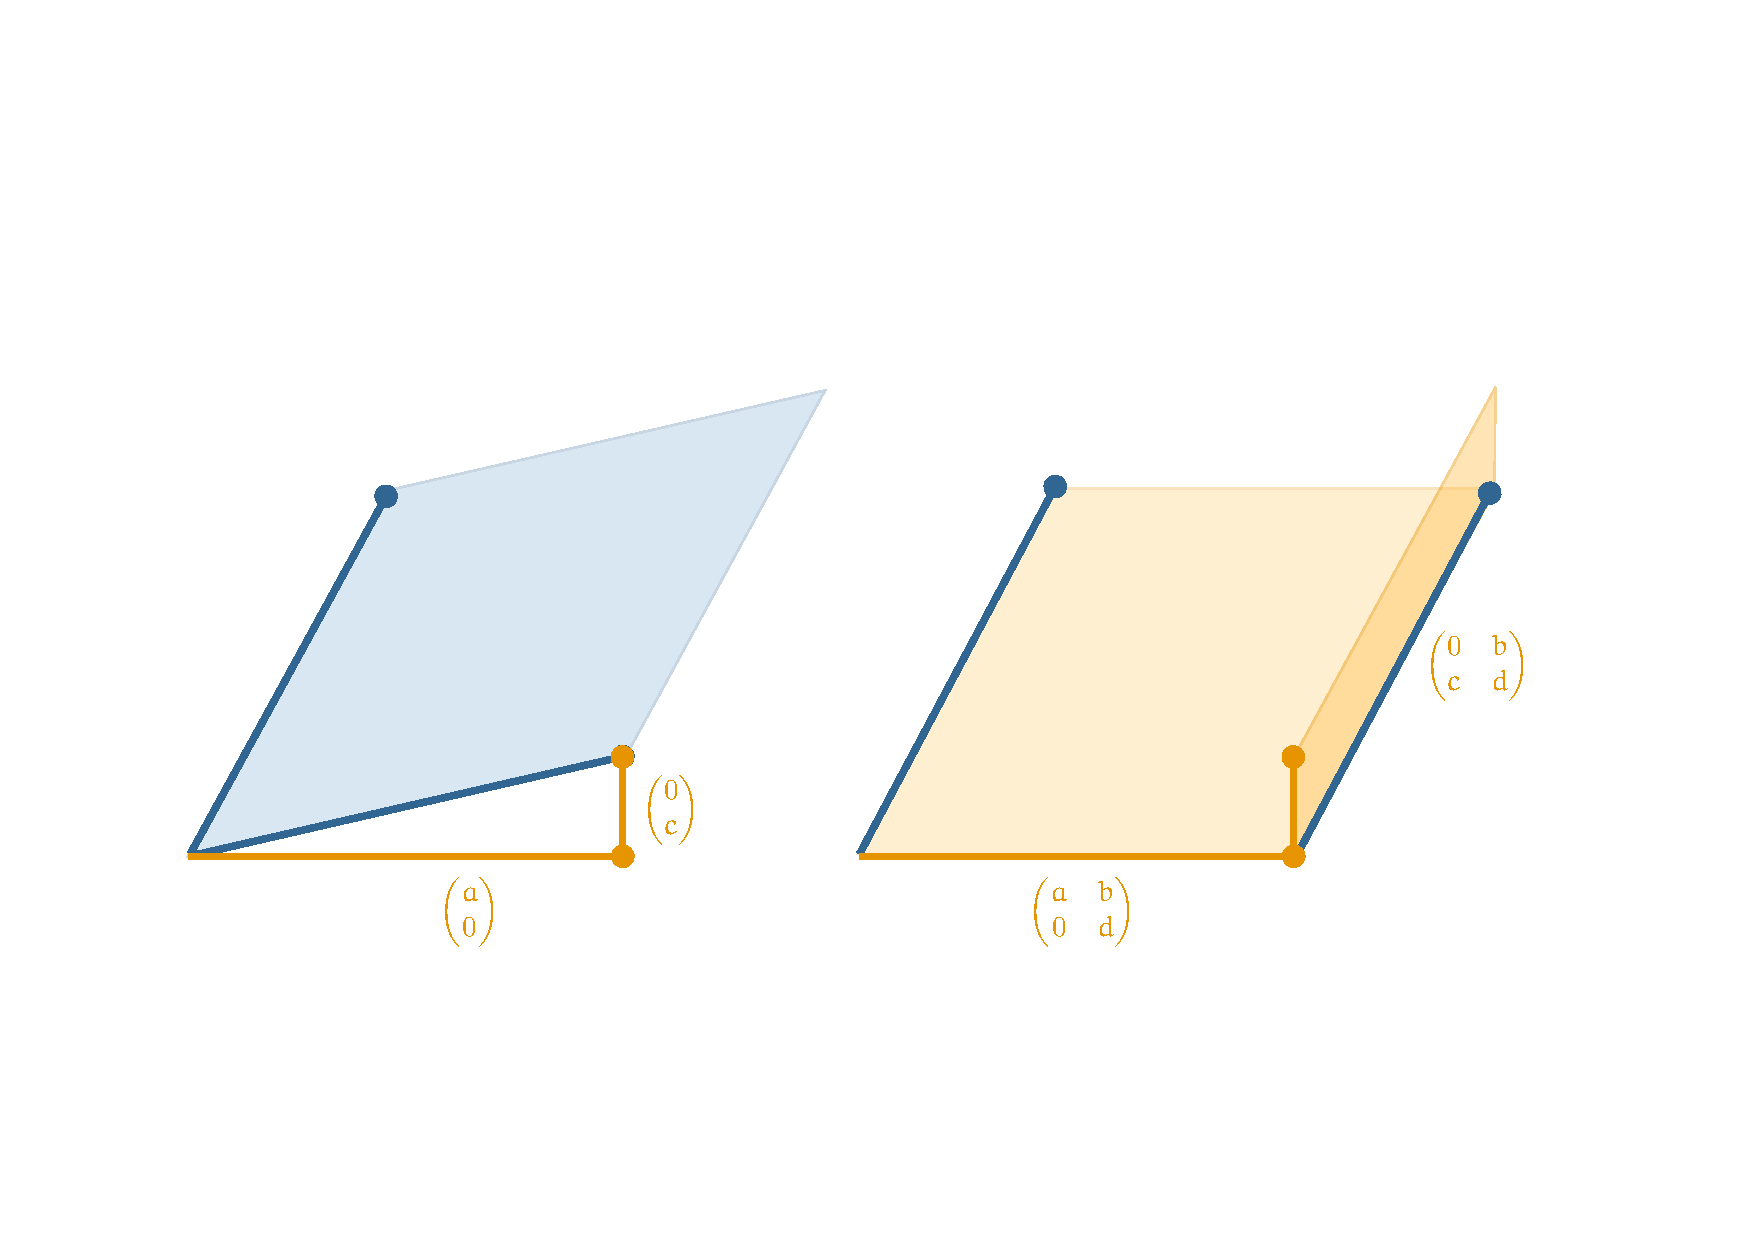
\includegraphics[width=1\textwidth]{./images/pca-3/determinant-step1.pdf}
	}
	\caption*{Breaking the determinant up in to two terms. Note that in the second image, the smaller parallelogram has negative area, because the two basis vectors are reversed.
	}
\end{figure}
%<figure class="narrow">
%<img src="/images/pca-3/determinant-step1.svg" />
%<figcaption>Breaking the determinant up in to two terms. Note that in the second image, the smaller parallelogram has negative area, because the two basis vectors are reversed.
%</figcaption>
%</figure>

Next, we use the property of skew invariance to subtract multiples of these new columns from the others. We use whatever multiple is required to make the rest of the row \(0\). The other rows are unaffected, since these all have \(0\)'s in the original column.

\index{Skew invariance}

\[
\left |\,\begin{matrix} a & b \\ \kc{0} & d\end{matrix}\;\right | + \left |\, \begin{matrix} \kc{0} & b \\ c & d\end{matrix} \;\right | = \left |\, \begin{matrix} a & \kc{0} \\ \kc{0} & d\end{matrix} \right | + \left |\, \begin{matrix} \kc{0} & b \\ c & \kc{0}\end{matrix} \right |\p
\]

Visually, that looks like this.

\begin{figure}[H]
	\centerline{
		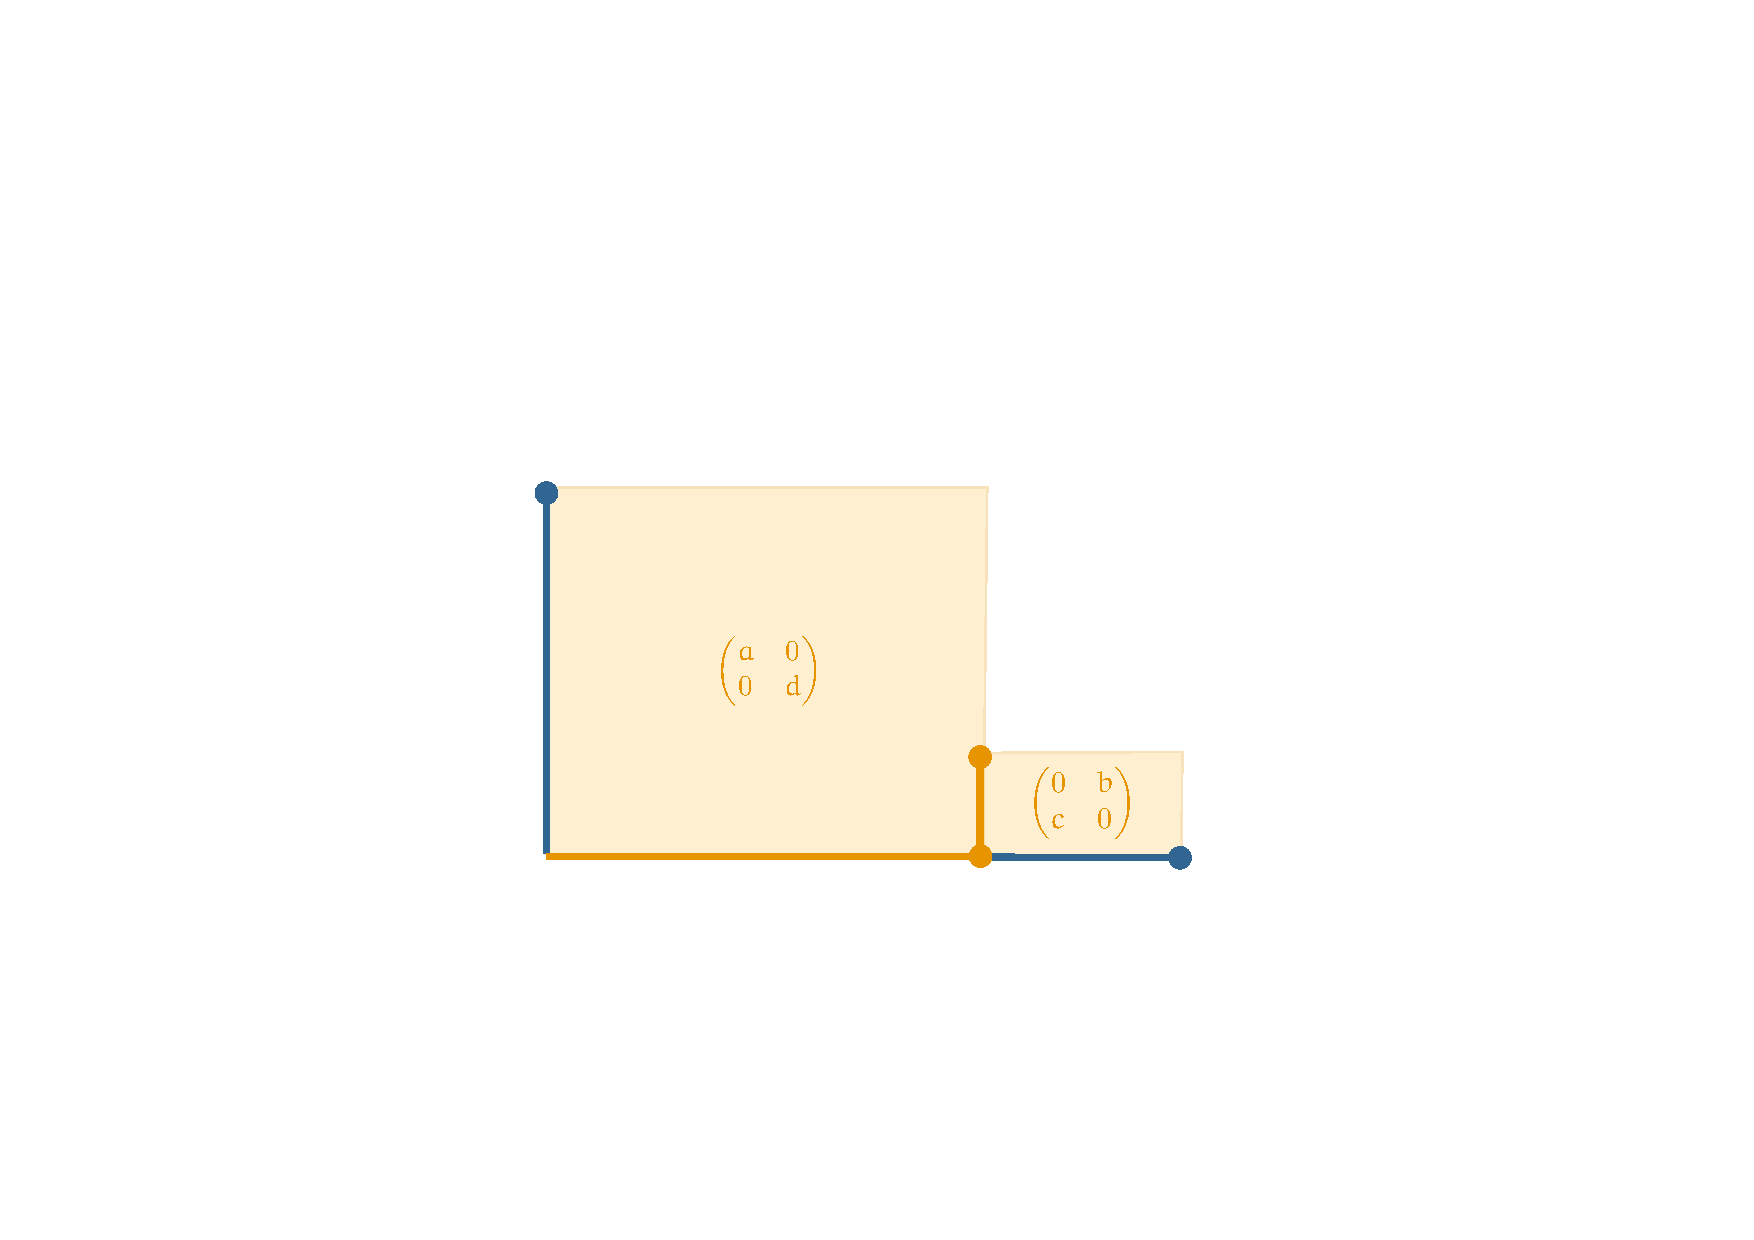
\includegraphics[width=0.8\textwidth]{./images/pca-3/determinant-step2.pdf}
	}
	\caption*{Axis-aligning the remaining basis vectors.
	}
\end{figure}

%<figure class="third center">
%<img src="/images/pca-3/determinant-step2.svg" />
%<figcaption>Axis-aligning the remaining basis vectors.
%</figcaption>
%</figure>

We have two parallelograms with one edge axis-aligned, and we simply skew them so that the other edge is axis-aligned as well. the area we're looking for is now the sum of two rectangles, one of which of facing away from us.

For the first term, we can work out the determinant easily. A diagonal matrix transforms the unit cube to a rectangle, so we just multiply the values along the diagonal: \(ac\). For the second term, we have an anti-diagonal matrix. We can turn this into a diagonal matrix by swapping the two columns. By the property of alternativity, this changes the sign of the area, so the resulting signed area is \(-bc\):

\index{alternativity}


\[
\left |\,\begin{matrix} a & \kc{0} \\ \kc{0} & d\end{matrix} \;\right | + \left |\, \begin{matrix} \kc{0} & b \\ c & \kc{0}\end{matrix} \;\right | \quad=\quad \left |\, \begin{matrix} a & \kc{0} \\ \kc{0} & d\end{matrix} \;\right | - \left |\, \begin{matrix} b & \kc{0} \\ \kc{0} & c\end{matrix} \;\right | \quad=\quad ac - bc \p
\]

This was certainly a more involved way of deriving the formula for the area of a polygon, but the benefit here is that this method generalizes to higher dimensions.

\subsection{Determinants for \(n\times n\) matrices}

We'll start with the three properties we used above, and see how they generalize to higher dimensions. 

\textbf{Skew invariance} also holds in higher dimensions. If we have an \(n \times n\) matrix \(\bc{\mbA}\) with \(n\) column vectors \(\bc{\mba}^1, \ldots, \bc{\mba}^n\), adding a multiple of one to another does not change the volume of the resulting parallelotope. For instance:

\index{Skew invariance}

\[
| \bc{\mbu}, \bc{\mbv}, \bc{\mbw} | = | \bc{\mbu} + \rc{r}\bc{\mbv}, \bc{\mbv}, \bc{\mbw} |
\]

\textbf{Multilinearity} also carries over in the same way. We can break one of the column vectors up into a linear combination of two (or more) other vectors and the area of the resulting paralellotope breaks up in the same way. For instance:
\index{Multilinearity}

\[
| \oc{\mbu}^1 + \oc{\mbu}^2, \bc{\mbv}, \bc{\mbw} | = | \oc{\mbu}^1 , \bc{\mbv}, \bc{\mbw} | + | \oc{\mbu}^2, \bc{\mbv}, \bc{\mbw} |
\]

Finally, \textbf{alternativity}. This requires a little more care. You'd be forgiven for thinking that since we have a higher-dimensional space, we now have more ways for our paralellotope to orient as well. We thought of our paralellogram as a piece of paper which could lie on the table in two ways. If we hold a parallellotope up in space, we can rotate it in all sorts of directions.

\index{Alternativity}

But the metaphor of a piece of paper is slightly misleading. When we flip a piece of paper upside-down, we rotate it, but that's not what really happens when we swap the basis vectors of the paralellogram. What really happens is that we turn the piece of paper inside-out: we \emph{flip} it by pulling the right edge to the left and the left edge to the right.

A better metaphor is a mirror: imagine standing in front of a mirror and holding up your right hand, palm forward.

It looks like your twin inside the mirror is holding up their left hand, with the thumb facing in the opposite direction. But if the mirror flips the image left-to-right, why doesn't it flip the image up-side-down as well? Why doesn't anything change if we turn the mirror ninety degrees?How does the mirror keep track of which direction the floor is?

\begin{figure}[p]
	\centerline{
		\hspace{3.5em}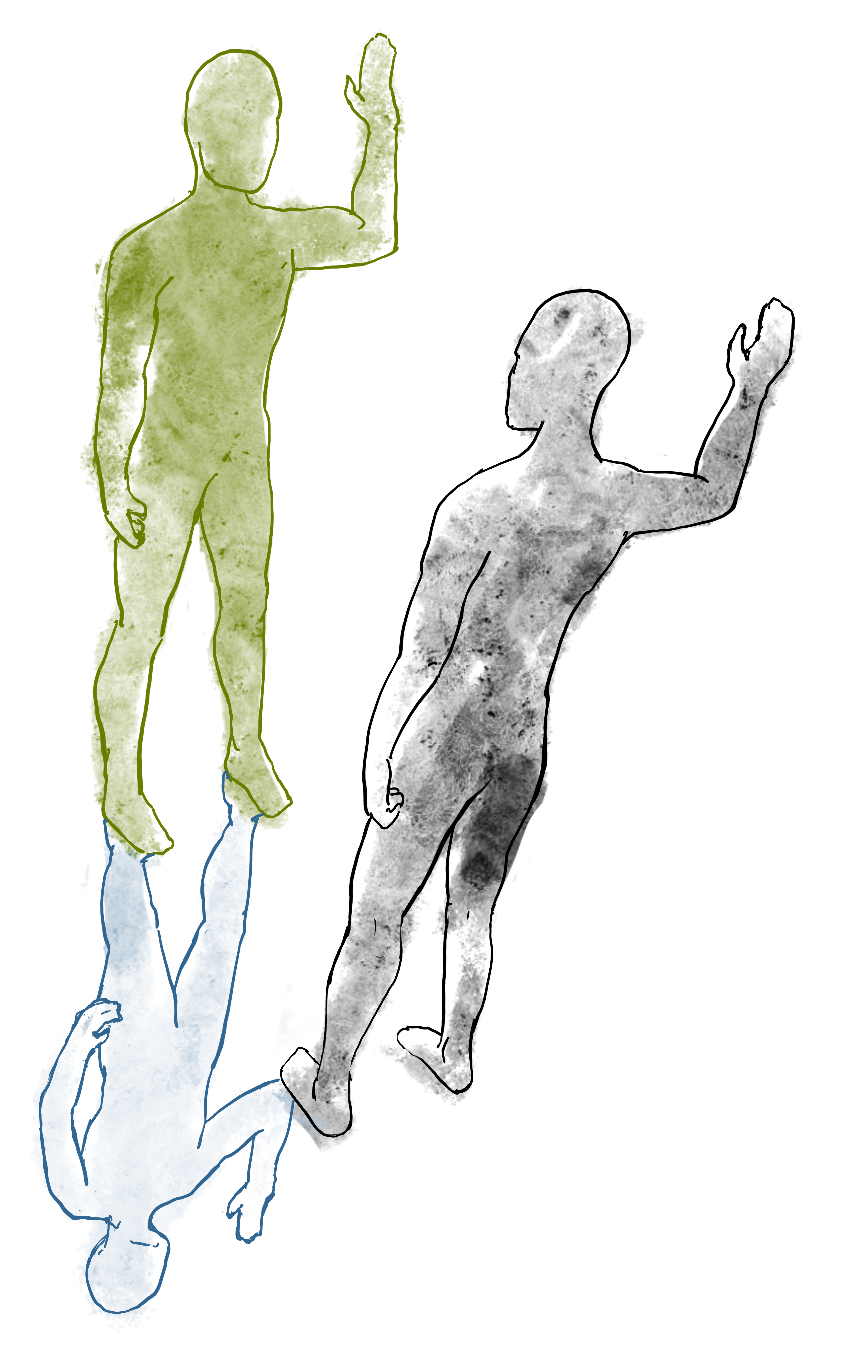
\includegraphics[width=0.8\textwidth]{./images/pca-3/mirrors.png}
	}
	\caption*{A mirror in front of you seems to flip you left-to-right, but it actually flips you \gc{back-to-front}. This \emph{also} turns your right hand into a left hand. A second mirror on the floor flips you \bc{upside-down}, turning your hand back into a right hand again.	}
\end{figure}


The answer is that the mirror \emph{doesn't} flip the image left-to-right. It flips it \emph{back-to-front}. In a manner of speaking, it pulls the back of your hand forward and the front of your hand backwards until the whole hand is flipped. 

\index{Mirror image}

%<figure class="centering">
%<img src="/images/pca-3/mirrors.png" class="three-quarters"/>
%<figcaption>A mirror in front of you seems to flip you left-to-right, but it actually flips you <span class="gc">back-to-front</span>. This also turns your right hand into a left hand. A second mirror on the floor flips you <span class="bc">upside-down</span>, turning your hand back into a right hand again.
%</figcaption>
%</figure>

Putting the mirror to your side will flip you left-to-right, also turning your right hand into a left hand. Putting the mirror on the floor and standing on it turns you upside-down, and again turns the right hand into a left hand. If you use two mirrors, one in front of you and one below, you are flipped back-to-front \emph{and} upside-down, and if you look at this mirror-twin, you'll see that their hand has been flipped twice, to become a right hand again.

The result is that we still have only two orientations. Each time anything gets mirrored, it gets pulled inside out along some line, and the sign of the volume changes: your right hand turns into a left hand and vice versa. If it gets flipped an even number of times the sign stays the same, and if it gets flipped an odd number of times, the sign changes.

This means that alternativity in higher dimensions is defined as follows: if we swap around any two columns in a matrix, we flip the space (along a diagonal between the two corresponding axes). Therefore, the magnitude of the determinant stays the same, but \emph{the sign changes}. If we flip two more axes, the sign changes back. For instance:

\index{Alternativity}

\[
|\; \mbu, \bc{\mbv}, \lbc{\mbw} \;| = - |\; \bc{\mbv}, \mbu, \lbc{\mbw} \;| = |\; \lbc{\mbw}, \mbu, \bc{\mbv} \;| \p
\]

That's our three properties in place. Finally, before we start our derivation, note that in the \(2 \times 2\) case, our ultimate aim was to work the matrix determinant into a sum of determinants of diagonal matrices. The idea was that the determinant of a diagonal matrix is easy to work out.

That's still true in higher dimensions: the columns of a diagonal matrix \(\bc{\mbA}\) each map one of the unit vectors to a a basis vector of length \(\bc{A}_{ii}\) that lies along the \(i\)-th axis. Together these form the sides of an \(n\)-dimensional ``brick'' whose volume is just these lengths multiplied together. So the plan stays the same: use our three properties to rewrite the determinant into a sum of determinants of diagonal matrices.

We'll work this out for a \(3 \times 3\) matrix explicitly as an example, but the principle holds for any number of dimensions.

We start by taking the first column of our matrix, and breaking it up into three simple vectors (using multilinearity).

\index{Simple vector}

\[
\left |\, \begin{matrix} ~a & b & c\\ d & e & f\\ g & h & i \end{matrix}\; \right | = 
\rc{\left |\, \begin{matrix} ~a & b & c\\ \kc{0} & e & f\\ \kc{0} & h & i \end{matrix}\; \right |} +
\gc{\left |\, \begin{matrix} ~\kc{0} & b & c\\ d & e & f\\ \kc{0} & h & i \end{matrix}\; \right |} +
\bc{\left |\, \begin{matrix} ~\kc{0} & b & c\\ \kc{0} & e & f\\ g & h & i \end{matrix}\; \right |}
\]

As before, we've broken our parallellotope into three parallellotopes, each with one of their edges axis-aligned. Next, we subract multiples of the first column from each of the other columns to turn the rows into vectors with only one non-zero element.

\index{Parallellotope}

\[
\rc{\left | \,\begin{matrix} a & \kc{0} & \kc{0}\\ \kc{0} & e & f\\ \kc{0} & h & i \end{matrix} \;\right |} +
\gc{\left | \,\begin{matrix} \kc{0} & b & c\\ d & \kc{0} &  \kc{0}\\ \kc{0} & h & i \end{matrix} \;\right |} +
\bc{\left | \,\begin{matrix} \kc{0} & b & c\\ \kc{0} & e & f\\ g & \kc{0} & \kc{0} \end{matrix} \;\right |}
\]

This doesn't yet look quite as simple as it did in our \(2 \times 2\) case, but we can go back to the first step and break the second column vector of each term into simple vectors as well. For the first term that looks like this:

\[
\rc{\left |\, \begin{matrix} ~a & \kc{0} & \kc{0}\\ \kc{0} & e & f\\ \kc{0} & h & i \end{matrix} \;\right |} = 
\rc{\left |\, \begin{matrix} ~a & \kc{0} & \kc{0}\\ \kc{0} & \kc{0} & f\\ \kc{0} & \kc{0} & i \end{matrix} \;\right |} + 
 \rc{\left |\, \begin{matrix} ~a & \kc{0} & \kc{0}\\ \kc{0} & e & f\\ \kc{0} & \kc{0} & i \end{matrix} \;\right |} +
 \rc{\left |\, \begin{matrix} ~a & \kc{0} & \kc{0}\\ \kc{0} & \kc{0} & f\\ \kc{0} & h & i \end{matrix} \;\right |}
\]

In the first term, one of the column vectors is zero. This means the parallelotope becomes a parallelo\emph{gram}, with \(0\) volume, so we can remove this term. For the other two, we apply the multilinear property to sweep the rows, and we get

\[
\rc{\left |\, \begin{matrix} ~a & \kc{0} & \kc{0}\\ \kc{0} & e & f\\ \kc{0} & h & i \end{matrix} \;\right |} = 
 \rc{\left |\, \begin{matrix} ~a & \kc{0} & \kc{0}\\ \kc{0} & e & \kc{0} \\ \kc{0} & \kc{0} & i \end{matrix} \;\right |} +
 \rc{\left |\, \begin{matrix} ~a & \kc{0} & \kc{0}\\ \kc{0} & \kc{0} & f\\ \kc{0} & h & \kc{0} \end{matrix} \;\right |}
\]

The logic is the same for the \gc{green} and \bc{blue} terms. If we ignore the zeros that we added, we end up with a \(2 \times 2\) submatrix, to which we can apply the same trick again to turn each term into two more terms. If we do this we get six terms in total.

\vspace{0.3em}
\begin{overlong}
 \rc{\left |\, \begin{matrix} a & \kc{0} & \kc{0}\\ \kc{0} & e & \kc{0} \\ \kc{0} & \kc{0} & i \end{matrix}\; \right |} +
 \rc{\left | \,\begin{matrix} a & \kc{0} & \kc{0}\\ \kc{0} & \kc{0} & f\\ \kc{0} & h & \kc{0} \end{matrix} \;\right |} +
 \gc{\left | \,\begin{matrix} \kc{0} & b & \kc{0} \\ d & \kc{0} &  \kc{0}\\ \kc{0} & \kc{0} & i \end{matrix} \;\right |} +
 \gc{\left | \,\begin{matrix} \kc{0} & \kc{0} & c\\ d & \kc{0} &  \kc{0}\\ \kc{0} & h & \kc{0} \end{matrix}\; \right |} +
 \bc{\left |\, \begin{matrix} \kc{0} & b & \kc{0}\\ \kc{0} & \kc{0} & f\\ g & \kc{0} & \kc{0} \end{matrix}\; \right |} + 
\bc{\left | \,\begin{matrix} \kc{0} & \kc{0} & c\\ \kc{0} & e & \kc{0}\\ g & \kc{0} & \kc{0} \end{matrix}\; \right |}
\end{overlong}
\vspace{0.7em}

\noindent The result is that we have separated the determinant into several terms, so that for each, the matrix in that term has only one non-zero element in each row and each column. The structure of the non-zero values is that of a \emph{permutation matrix}, with the exception that permutation matrices contain only \(1\)s and \(0\)s. These are like the original matrix \(
\bc{\mbA}\) with a permutation matrix used to mask out certain values.

\index{Permutation matrix}

In fact, what we have done is to enumerate \emph{all possible permutations}. We started by creating one term for each possible choice for the first column, and then for each term we separated this in to the remaining two choices for the second column (after which the choice for the third column was fixed as well).

\index{Permutation}

This idea naturally generalizes to higher dimensions. Moving from left to right, we pick one element of each column and zero out the rest of its column and row. At each subsequent step we limit ourselves to whatever non-zero elements remain. We sum the determinants of all possible ways of doing this.

\noindent We can now turn each of these matrices into a diagonal matrix, by swapping around a number of columns. By the property of alternativity, this doesn't change the magnitude of the determinant, only the sign: for an even number of swaps, it stays the same and for an odd number it flips around. This gives us 

\vspace{0.3em}
\begin{overlong} \rc{\left| \,\begin{matrix} a & \kc{0} & \kc{0}\\ \kc{0} & e & \kc{0} \\ \kc{0} & \kc{0} & i \end{matrix}\; \right |} -
 \rc{\left | \,\begin{matrix} a & \kc{0} & \kc{0}\\ \kc{0} & f & \kc{0} \\ \kc{0} & \kc{0} & h\end{matrix}\; \right |} -
 \gc{\left |\, \begin{matrix} b & \kc{0} & \kc{0} \\ \kc{0} & d & \kc{0}\\ \kc{0} & \kc{0} & i \end{matrix}\; \right |} +
 \gc{\left | \,\begin{matrix} c & \kc{0} & \kc{0} \\  \kc{0} & d &  \kc{0}\\ \kc{0} & \kc{0} & h \end{matrix}\; \right |} +
 \bc{\left |\, \begin{matrix} b & \kc{0}  & \kc{0}\\ \kc{0} & f & \kc{0} \\ \kc{0} & \kc{0} & g \end{matrix} \;\right |} - 
\bc{\left |\, \begin{matrix} c & \kc{0} & \kc{0} \\ \kc{0} & e & \kc{0}\\ \kc{0} & \kc{0} & g\end{matrix} \;\right |} 
\p
\end{overlong}
\vspace{0.7em}

\noindent And since the determinant of a diagonal matrix is simply the diagonal product, as we worked out earlier, we get

\[
\left |\,\begin{matrix} a & b & c\\ d & e & f\\ g & h & i \end{matrix} \; \right | =
\rc{aei} - \rc{afh} - \gc{bdi} + \gc{cdh} + \bc{bfg} + \bc{ceg} \p
\]

To generalize this to \(n\) dimensions, we represent a permutation of the first \(n\) natural numbers with the symbol \(\sigma\). For instance, if \(n=6\) we may have \(\sigma = \langle 1, 5, 4, 3, 2\rangle\). We'll call the \emph{sign} of a permutation, \(\text{sign}(\sigma)\), \(-1\) if the permutation can be placed in the correct order with an odd number of swaps and \(1\) if this can be done with an even number of swaps.

%Then, for a given \(n \times n\) matrix \(\bc{\mbA}\), let \(\bc{\mbA}^\sigma\) be the matrix constructed by taking \(\bc{\mbA}\) and zeroing out any element that doesn't have an index of the form \((\sigma_i, i)\). That is, iterate over the columns \(i\), mark the element in that column at row \(\sigma_i\), and zero out the rest.

 
Then, the process we described above leads to the following formula for the determinant:

\[
|\bc{\mbA}| = \sum_\sigma \text{sign}(\sigma) \prod_i \bc{A}_{\sigma(i), i}
\]

where the sum is over all permutations of the first \(n\) natural numbers, and the product runs from \(1\) to \(n\).

Note that for each term in our sum, corresponding to the permutation \(\sigma\), the value \(\bc{A}_{\sigma(i), i}\) marks out one of the elements that we haven't zeroed out. The value \(\prod_i \bc{A}_{\sigma(i), i}\) is the product of all these values.


This is called the \textbf{Leibniz formulation} of the determinant. 

\index{Leibniz formulation}\index{Determinant!Leibniz formulation}

\begin{aside}We got here by defining the determinant as the volume of a parallelotope and then deriving the Leibniz formulation from that. This is useful for building a visual intuition, but if you want to be rigorous it's not the most efficient approach.

For this reason, the determinant is usually first defined as \emph{any} multilinear, alternative function, which yields 1 for the identity matrix. You can then show that there is only one such function, and that it's the Leibniz function above. From there, you can then prove all the other interpretations of the determinant, including the geometrical one.
\end{aside}

%<!-- 
%
%### Computing determinants for \(n\times n\) matrices: Laplace expansion
%
%How do we scale this up to higher dimensions? For \(n\times n\) matrices, computing the determinant is not quite as simple as subracting one diagonal product from another. Geometrically, the principle is the same: in three dimensions, we transform the unit cube into a parallelepiped (a 3D parallelogram) and work out its volume. In \(n\) dimensions we transform a hypercube into the n-dimensional equivalent of a paralellogram, called a _parallelotope, and work out its hypervolume. The drawback here is that the formulae for these (hyper)volumes are not straightforward.
%
%Here's some intuition to help us along. The sides of a parallelepiped are parallellograms. The sides of a 4D parallelotope are paralellepipeds, and so on. Can we somehow build up from what we know, using the formula for area to compute the volume and then use the formula for volume to compute the 4D volume and so on?
%
%This is the basis behind the _Laplace expansion_. We take the \(n \times n\) matrix for whcih we want to compute the determinant, slice out a number of matrices of one "dimension" lower (\(n-1 \times n-1\) matrices), compute _their_ determinants, and then work out the determinant of the original matrix as a function of these.
%
%The Laplace expansion is a recursive algorithm: given an \(n \times n\) matrix, we slice out a series of \((n-1) \times (n-1)\) matrices, compute _their_ determinants, and then combine them to compute the determinant of the  \(n \times n\) matrix. How do we compute the determinants of the smaller matrices? We uses their Laplace expansions (slicing out \((n-2) \times (n-2) matrices)\) and so on, until the slices are \(2 \times 2\) and we can use the simple function we discovered above.
%
%<p>Here's how it works in detail. Given an \(n \times n\) matrix \(\bc{\A}\), let \(\bc{\A}^{ij}\) be the result of removing the \(i\)-th row and \(j\)-th column of \(\bc{\A}\). This is called a <em>minor</em> of \(\bc{\A}\). Since we've removed one row and one column, each minor is an \((n-1) \times (n-1)\) matrix.</p>
%
%<aside>Note the boldface: \(\bc{\A}^{ij}\) is a matrix, whereas \(\bc{A}_{ij}\) is a scalar (one element of \(\bc{\A}\)).
%</aside>
%
%Fixing row \(i=\rc{1}\) and iterating over the columns \(\gc{j}\), we can now compute the determinant as
%
%\[
%\text{det}\;\bc{\A} = \bc{A}_{\rc{1}\gc{1}}\text{det}\bc{\A}^{\rc{1}\gc{1}} - \bc{A}_{\rc{1}\gc{2}}\text{det}\; \bc{\A}^{\rc{1}\gc{2}} + \bc{A}_{\rc{1}\gc{3}}\text{det}\; \bc{\A}^{\rc{1}\gc{3}} + \ldots \pm \bc{A}_{\rc{1}\gc{n}}\text{det}\;\bc{\A}^{\rc{1}\gc{n}} \p
%\]
%
%Note that the sign of the terms alternates, so the last term is positive or negative depending on whether \(n\) is odd or even.
%
%<aside> The choice of row is arbitrary. It works with any other row \(i\) too, so long as the term for each minor \(\bc{\A}^{ij}\) is positive if \(i+j\) is even and negative if it is odd.
%</aside>
%
%We can apply this method recursively until the matrices are \(2 \times 2\), and then work backwards from there. 
%
%It's not very intuitive why this method should work to give us the determinant. Laplace himself most likely worked this out by taking _Cramer's rule_, an equality containing the minors of a matrix and the determinant, and rewriting the terms. For our purposes, that adds even more baggage, and it takes us away from the neat geometric interpretation of the \(2 \times 2\) case. 
%
%Can we work out a similarly geometric interpretation for the Laplace's formula? It turns out that you can, with relative ease, using something called _Geometric algebra_. This is a bit of a diversion, so I've moved it to the appendix. If you're happy to take Laplace at his word, then read on, but if you have the time, geometric algebra is an extremely useful generalization in geometry.
% -->
%
%<!-- The determinant is a very useful tool, but we need it only for one purpose: to tell us which matrices are invertible. The reason we need this is because it allows us to relate the eigenvalues of a matrix to the roots of a particular polynomial defined from a matrix, called the characteristic polynomial. -->


The determinant is a powerful tool, with many uses. Here, we only care about one of them: \emph{it lets us characterize whether a matrix is invertible or not}. The determinant is precisely zero if and only if the matrix is not invertible. The reason we care about this, is that it will lead to a very useful way of characterizing the eigenvalues: the \textbf{characteristic polynomial} of a matrix.

\section{The characteristic polynomial}
\index{Characteristic polynomial}

Let's start with how we originally characterized eigenvalues in Chapter~\ref{chapter:eigenvectors}. There, we said that an eigenvector of a matrix \(\bc{\mbA}\) is any vector \(\rc{\mbv}\) for which the direction doesn't change, under operation of the matrix. The magnitude \emph{can} change, and the increase of that magnitude we call the eigen\emph{value} \(\bc{\lambda}\) corresponding to the eigenvector.

To summarize, for any eigenvector \(\rc \mbv\) and its eigenvalue \(\bc{\lambda}\) of \(\bc \mbA\), we have

\[
\bc{\mbA}\rc{\mbv} = \bc{\lambda}\rc{\rc{\mbv}} \p
\]

Moving the right-hand-side over to the left, we get 

\[
\bc{\mbA}\rc{\mbv} - \bc{\lambda} \rc{\mbv} = {\mathbf 0} \text{,}
\]

where both sides are vectors, with a vector of zeros on the right. To allow us to manipulate the left hand side further we rewrite \(\bc{\lambda}\rc{\mbv}\) as \((\bc{\lambda}\mbI)\rc{\mbv}\). This gives us:

\begin{align*}
\bc{\mbA}\rc{\mbv} - \bc{\lambda}\mbI\rc{\mbv} &= {\mathbf 0}  \\
(\bc{\mbA} - \bc{\lambda}\mbI)\rc{\mbv} &= {\mathbf 0} \p 
\end{align*}

This last line is basically a linear problem of the form \(\bc{\mbM}\rc{\mbv} = \mathbf 0\), with \(\bc{\mbM} = (\bc{\mbA} - \bc{\lambda}\mbI)\). The solutions to this problem, the set of all vectors \(\rc \mbv\) that we can multiply by \(\bc{\mbM}\) to get the null vector \(\mathbf 0\) are called the \emph{null space} of \(\bc{\mbM}\). What we have just shown is that \textbf{any eigenvector of \(\bc \mbA\) with eigenvalue \(\bc \lambda\) must be in the null space of the matrix \(\bc{\mbA} - \bc{\lambda}\mbI\)}.

This is where invertibility and the determinant come in: if \(\bc \mbM\) is invertible, it can only map one point to any other point. Every matrix maps \(\mathbf 0\) to \(\mathbf 0\), so for any invertible matrix the null space consists only of the point \(\mathbf 0\). The only matrices with more interesting null spaces are non-invertible matrices. Or, matrices with determinant \(0\). 

\begin{aside}%
Note that we're not talking about the invertibility of \(\bc \mbA\) itself, only of the derived matrix \(\bc{\mbM} = \bc{\mbA} - \bc{\lambda}\mbI\)
\end{aside}

So, now we can tie it all together. Choose some scalar value \(\bc \lambda\). If we have 

\[\left | \; \bc{\mbA} - \bc{\lambda}\mbI \;\right | = 0\]

then the matrix \(\bc{\mbA} - \bc{\lambda}\mbI\) has a non-trivial null-space, and \(\bc \lambda\) is an eigenvalue. We want to study the left-hand-side of this equation as a function of \(\bc{\lambda}\), taking the values in \(\bc{\mbA}\) as constants.

As we've seen, expanding the determinant into an explicit form can get a little hairy for dimensions larger than 3, but we don't need to make it explicit, so long as we can tell what \emph{kind} of function it is. To illustrate, say we have a \(2 \times 2\) matrix 

\[
\bc \mbA = \begin{pmatrix}a & b \\ c & d\end{pmatrix} \p
\]

In that case, the value \(\left |\,\bc{\mbA} - \bc{\lambda}\mbI\,\right|\) works out as

\[
(a-\bc{\lambda})(d - \bc{\lambda}) - bc \p
\]

We can multiply out these brackets, and we would see that this is a polynomial with \(\bc{\lambda}\) as its variable. This polynomial has \(\bc{\lambda}^2\) as the highest power. The values for which this polynomial equal zero, its \textbf{roots}, are the eigenvalues of the original matrix \(\bc{\mbA}\).

\noindent For an \(n\times n\) matrix, as we saw, the Leibniz form of the determinant gives us one term for each possible permutations of length \(n\), each of which consists of \(n\) elements of the matrix multiplied together. If any of these elements come from the diagonal, they contain \(\bc{\lambda}\). That means each term contains at most \(n\) \(\bc{\lambda}\)s, giving us an \(n\)-th order polynomial.

As you may have guessed, this function is what we call the \textbf{characteristic polynomial} of \(\bc{\mbA}\). The points where this function is \(0\), the roots of the polynomial, are the eigenvalues of \(\bc{\mbA}\). 

And this means that we can apply a whole new set of tools from the analysis of polynomials, to the study of eigenvectors. We never have to work out the characteristic polynomial explicitly, we can just use the knowledge that the determinant \emph{is a polynomial} and use what we know about polynomials to help us further along towards the spectral theorem.

And one of the richest and most versatile tools to come out of the analysis of polynomials, is the idea of \emph{complex numbers}. This is a counterintuitive idea, so we'll take some time to set it up carefully, before we dig into the mathematics.

\section{Complex numbers}
\index{Complex numbers}

Complex numbers spring from the idea that there exists a number \(i\) for which \(i^2\) is \(-1\). We don't know of any such number, but we simply assume that it exists, and investigate the consequences. For many people this is the point where mathematics becomes too abstract and they tune out. The idea that squares can be negative clashes too much with our intuition for what squares are. The idea that we just pretend that they can be negative and keep going, seems almost perverse.

And yet, this approach is one that humanity has followed again and again in the study of numbers. If you step back a bit, you start to see that it is actually one of the most logical and uncontroversial things to do. 

The study of numbers started somewhere before recorded history, in or before the late stone age, when early humans began counting things in earnest, and they learned to \emph{add}. I have five apples, I steal three apples from you, now I have eight apples. That sort of thing.

\noindent At some point, these early humans will have solidified their concept of ``numbers.'' It is a set of concepts (whose meaning we understand intuitively) which starts \(1, 2, 3, \ldots\) and continues. If you add one number to another, you always get another number.  If the number was big, they may not have had a name for it, but a patient paleolithic human with enough time could certainly have carved the required number of tally marks into an animal bone.

The operation of addition can also be reversed. If \(5 + 3\) gives \(8\), then taking \(5\) away from \(8\) gives \(3\). If I steal \(5\) apples from your collection of \(8\), you still have \(3\) left. Thus, subtraction was born. But subtraction, the \emph{inverse} of addition, required some care. Where adding two numbers always yields a new number, subtracting two numbers doesn't always yield a new number. You can't have \(5 - 8\) apples, because if you have \(5\) apples I can't steal more than \(5\) of them.

As societies grew more complicated, financial systems developed and \emph{debt} became an integral part of daily life. At some point, the following thought experiment was considered. What if \(5-8\) is a number after all? Maybe it's just a number we don't have a name for yet.

So, we'll just give it a name and see if we can make some sense of how it behaves. No doubt many people were outraged by such a suggestion, protesting that it was unnatural, and an insult to whatever God they believed had designed the numbers. But simple investigation soon showed that if these numbers were assumed to exist, they followed simple rules and, it made sense to think of them as a kind of mirror image of the natural numbers, extending to infinity in the opposite direction. \(5 - 8\) was the mirror image of \(3\), so it made sense to call it ``\(-3\)''.

\index{Negarive numbers}

The skeptics might argue that this made no sense, because there is no such thing as having \(-3\) apples, but the mathematicians will have countered that in other areas, such as finance, there were concepts that could be expressed very beautifully by the negative numbers. If I owe you \(3\) apples, because my earlier theft was found out, but you also stole \(8\) apples from me, I now owe you \(-5\) apples, or rather, you owe me \(5\).

The same principle can be applied to multiplication. If your tribe has \(8\) families, and every family is entitled to \(5\) apples, you need to find \(8 \times 5\) apples. Again, an operator, and any two numbers you care to multiply will give you a new number (even if you believe in negative numbers).

And again, you can do the reverse the operation: if the harvest has yielded \(48\) apples, you can work out that every family in your tribe gets \(6\) of them. But again, you have to be careful about which numbers you apply the inverse to. Sometimes you get a known number, and sometimes you don't. If you have 50 apples, suddenly there is no known number that is the result of \(50/8\).

But what if there was? What if we just gave \(50/8\) a name and started investigating? We'd find out pretty quickly that it would make sense to think of these numbers as lying \emph{in between} the integers. We call these the \emph{rational} numbers. Whoever it was that invented the rationals must have run into less resistance than the inventor of the negative numbers; it's much easier to imagine half an apple than to imagine \(-3\) of them.

The pattern is hopefully becoming clear. Let's have one more example, to really drive the point home, and also to bring us far enough into recorded history so we can actually see how people dealt with these revelations. Adding is repeated counting, and multiplication is repeated adding so \emph{raising to a power}, repeated multiplication, is the next operator in the hierarchy. 

The story should be familiar at this point. Any two natural numbers \(a\) and \(b\) can be "exponentiated" together as \(a^b\) and the result is another natural number.

\index{Exponentiation}

The inverse operation is a b-th root, but we can stick with square roots to illustrate our point. In fact the square root of 2, the length of the diagonal of a unit square, is all we need. In this case, there is nothing abstract or perverse about the quantity \(\sqrt 2\): in a square room with sides of 1 meter it's the distance from one corner to the corner opposite.
\enlargethispage{4em}

\begin{figure}[H]
	\centerline{
		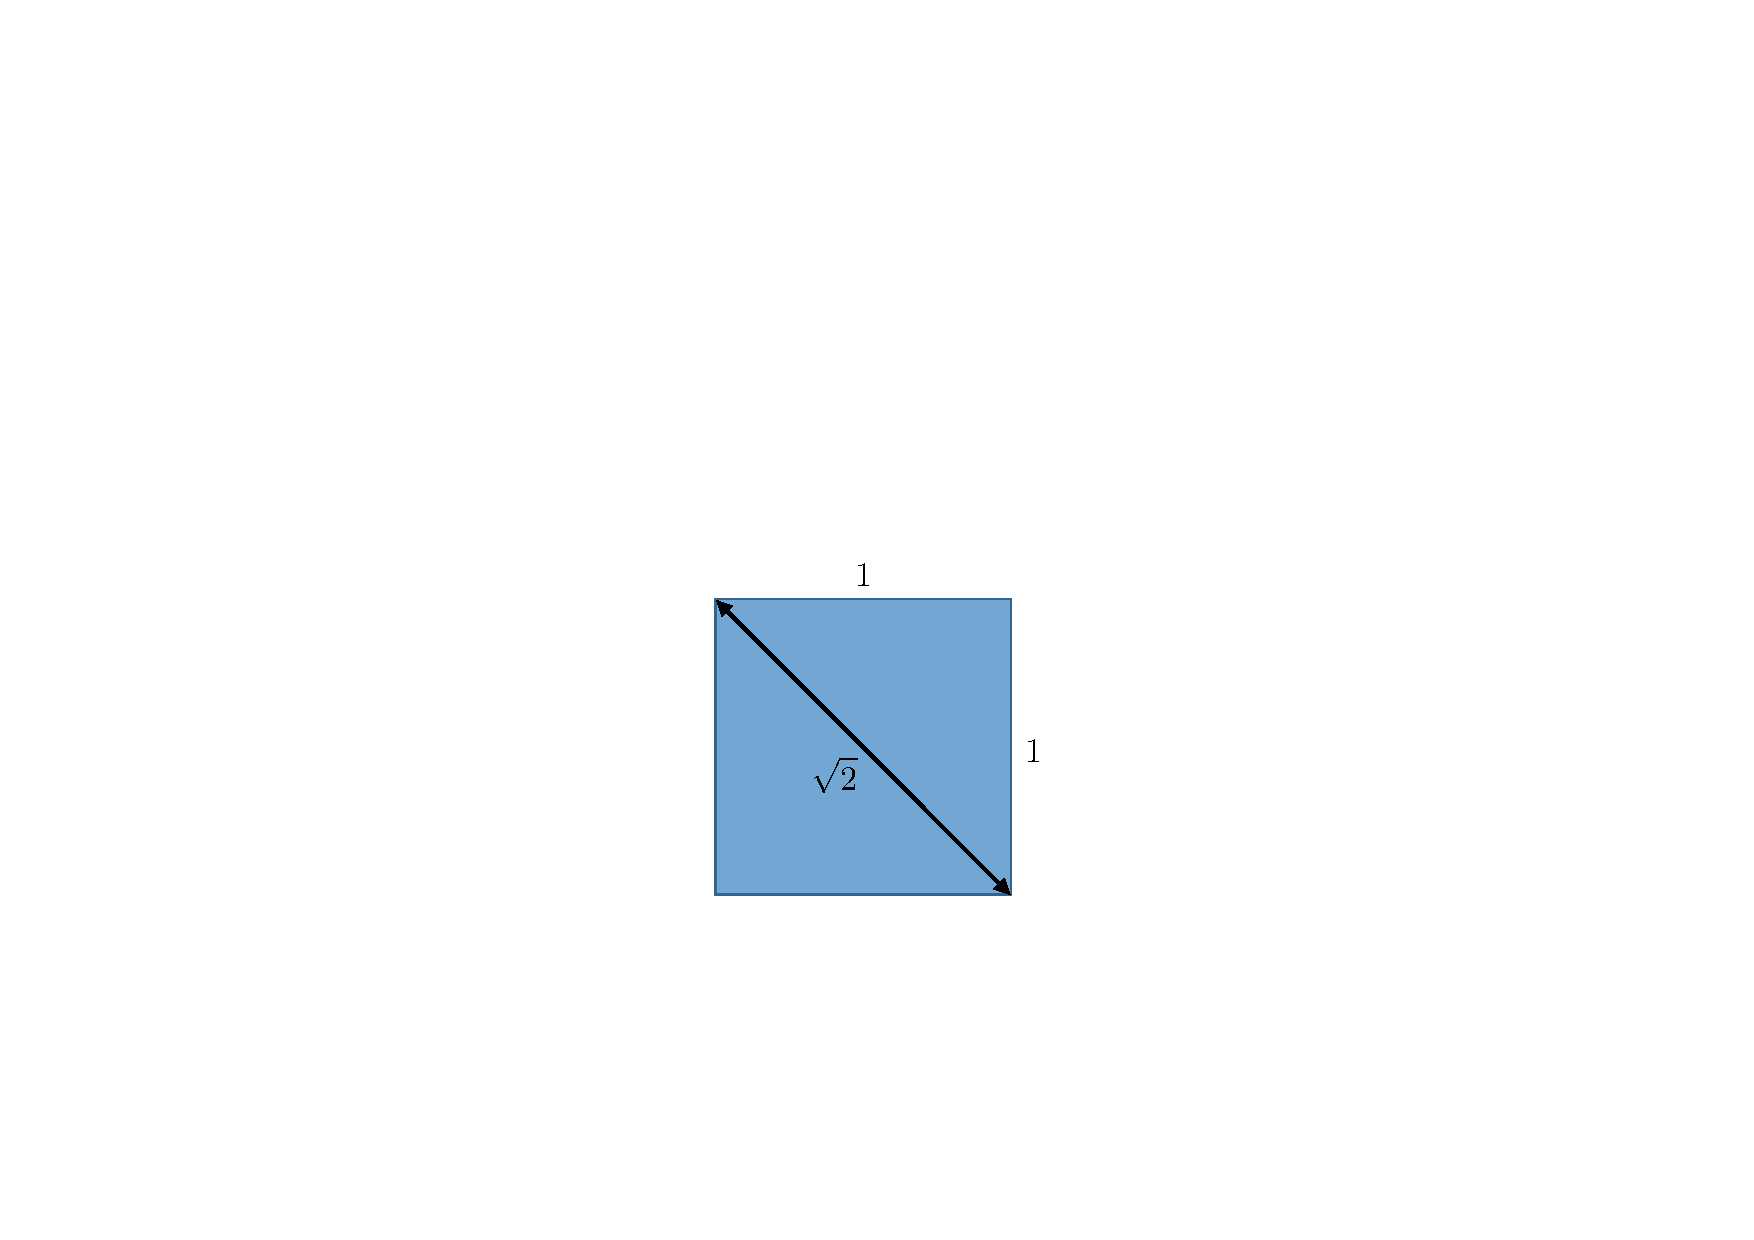
\includegraphics[width=0.4\textwidth]{./images/pca-3/sqrt2.pdf}
	}
\end{figure}

%<figure class="centering">
%<img src="/images/pca-3/sqrt2.svg" class="tile4"/>
%<figcaption>
%</figcaption>
%</figure>

And yet, when people investigated, it caused great upset.

The man who gave his name to the theorem we would use to work out the above picture, Pythagoras, was the head of a cult. A cult dedicated to mathematics. They lived ascetically, much like monks would, centuries later, and dedicated themselves to the study of nature in terms of mathematics. When asked what the purpose of man was, Pythagoras answered ``to observe the heavens.'' One fervent belief of the Pythagoreans was that number and geometry were inseparable: all geometric quantities could be expressed by (known) numbers.

\index{Pythagoras}\index{Pythagoreans}

The story of the Pythagoreans is a mathematical tragedy. It was one of their own, commonly identified as Hippasus of Metapontum, who showed that no rational number corresponded exactly to \(\sqrt{2}\). Some aspects of geometry were outside the reach of the known numbers. According to legend, he was out at sea when he discovered this, and was promptly thrown overboard by the other Pythagoreans.

\index{Hippasus of Metapontum}

Of course, with the benefit of hindsight, we know how to manage such upsetting discoveries. We simply give the new number a name, ``\(\sqrt{2}\),'' and see if there's some place among the numbers where it makes sense to put it. In this case, somewhere between \(141/100\) and \(142/100\), in a space we can make infinitely small by choosing better and better rational approximations.

With this historical pattern clearly highlighted, the discovery of the complex numbers should be almost obvious. In fact, we don't even need a new operation to invert, we are still looking at square roots, but instead of applying the square root a positive integer, we apply it to a \emph{negative integer}. To take the simplest example, we'll look at  \(\sqrt{-1}\). No number we know gives \(-1\) when we multiply it by itself, so our first instinct is to dismiss the operation. The square root is only allowed for a subset of the real-valued numbers. Just like subtraction was only allowed for a subset of the natural numbers, and division was only allowed for a subset of the integers.

But, what if the number \(\sqrt{-1}\) did exist? What would the consequences be?

As the previous paragraphs should illustrate, this kind of investigation is usually born out of necessity. Like a fussy child given a new food, people are consistently reluctant to accept new types of numbers. In this case, what pushed us over the edge was the study of polynomials; functions of the form: 

\[f(x) = \bc{a}x^3 + \bc{b}x^2 + \bc{c}x + \bc{d}\] 

where the highest exponent in the sum indicates the \emph{order} of the polynomial.

The problem of finding the \emph{roots} of a polynomial, the values of \(x\) for which \(f(x)\) is equal to \(0\) crops up in all sorts of practical problems. In some cases, this leads to squares of negative numbers, as we see when we try to solve \(\gc{x^2 + 1 = 0}\). This didn't worry anybody, of course, since this function lies entirely above the horizontal axis---it has no roots---so it's only natural that solving for the roots leads to a contradiction. 

\index{Roots of a polynomial}\index{Polynomial!roots of}

\begin{figure}[H]
	\centerline{
		\includesvg[width=0.8\textwidth]{./images/pca-3/polynomials.svg}
	}
	\caption*{The function \(f(x) = x^2 + 1\) has no roots: it doesn't cross the horizontal axis. Therefore, it make sense that \(x^2 = 0\) or \(\sqrt{-1}\) has no solutions.	}
\end{figure}

%<figure class="half center">
%<img src="/images/pca-3/polynomials.svg">
%<figcaption>The function \(f(x) = x^2 + 1\) has no roots. This makes total sense, since it doesn't cross the horizontal axis.
%</figcaption>
%</figure>

However, when people started to work out general methods for finding the roots of \emph{third}-order polynomials, like \(\bc{x^3 - 15x - 4}\), which \emph{does} have roots, it was found that the methods worked if one temporarily accepted \(\sqrt{-1}\) as an intermediate value, which later canceled out. This is where the phrase \emph{imaginary} number originates. People (Descartes, to be precise) were not ready to accept these as numbers, but no one could deny their utility.

\index{Descartes}

Eventually, people followed the pattern that they had followed for the integers, the rationals and all their successors. We give the new number a name, \(i = \sqrt{-1}\), and we see if there's any way to relate it, geometrically, to the numbers we know.

Let's start with addition. What happens if we add \(i\) to some number, say \(3\)? The simple answer is that nothing much happens. The most we can say about the new number is that it is \(3 + i\). 

\index{Complex numbers!addition}

Multiplication then. Again \(2 \times i\) doesn't simplify in any meaningful way, so we'll just call the new number \(2i\). What if we combine the two? With a few subtleties, we can rely on the basic rules of algebra to let us multiply out brackets and add things together. So, if we start with \(i\), add 3 and multiply by 2, we get:

\index{Complex numbers!multiplication}

\begin{align*}
2(i + 3) = 2\cdot3 + 2\cdot i = \bc{6} + \rc{2}i 
\end{align*}

This is a very common result: we've applied a bunch of operations, involving the imaginary number \(i\), and the result can be written as the combination of a real value \(\bc{r}\), another real value \(\rc{c}\) and \(i\) as:

\[
\bc{r} + \rc{c}i \p
\]

\index{Complex numbers!Cartesian notation}

We will call any number that can be written in this way a \emph{complex number}. The set of all complex numbers is written as 

\[{\Large \mathbb C} \p\]

\index{\(\mathbb C\)}

At this point you may be worried. What if we come up with another operation that is not defined for all complex numbers? Are we going to have to make another jump? Are we going to find ever bigger families of numbers to deal with? It turns out that in many ways, \(\mathbb C\) is the end of the line. So long as we stick to algebraic operations, we can do whatever we like to complex numbers, and the result will always be well defined as another complex number.

\pagebreak 

% !!!
%\setlength\parfillskip{0pt plus .6\textwidth}
%\setlength\emergencystretch{2pt}

\noindent To illustrate, let's show this for a few simple examples. Lets say we have two complex numbers \(\gc{a} + \gc{b}i\) and \(\oc{c} + \oc{d}i\). If we add them, we get

\[(\gc{a} + \gc{b}i) + (\oc{c} + \oc{d}i) = \gc{a} + \oc{c} + \gc{b}i + \oc{d}i = \bc{(a + c)} + \rc{(b + d)}i
\]

\index{Complex numbers!addition}

If we multiply them, we get

\begin{align*}
(\gc{a} + \gc{b}i)(\oc{c} + \oc{d}i) &= \gc{a}\oc{c} + \gc{a}\oc{d}i + \gc{b}i\oc{c} + \gc{b}i\oc{d}i \\
&= (\gc{a}\oc{d} + \gc{b}\oc{d}\kc{i^2}) + (\gc{a}\oc{d} + \gc{b}\oc{c})i \\
&= \bc{ad - bd} + \rc{(ad + bc)}i \p
\end{align*}

That is, one \bc{real-valued number}, added to \(i\) times another \rc{real-valued number}. Note that in the second line of the derivation for the multiplication, we can use \(\kc{i^2} = -1\), since we know that \(i = \sqrt{-1}\). In short, multiplying or adding together any two complex numbers gives us another complex number. 

\index{Complex numbers!multiplication}

Since every complex number can be written as the combination of two real-valued numbers, it makes sense to visualize them in a plane. We plot the value of the \bc{real term} along the horizontal axis and the value of the \rc{imaginary term} along the vertical. 

\begin{figure}[H]
	\centerline{
		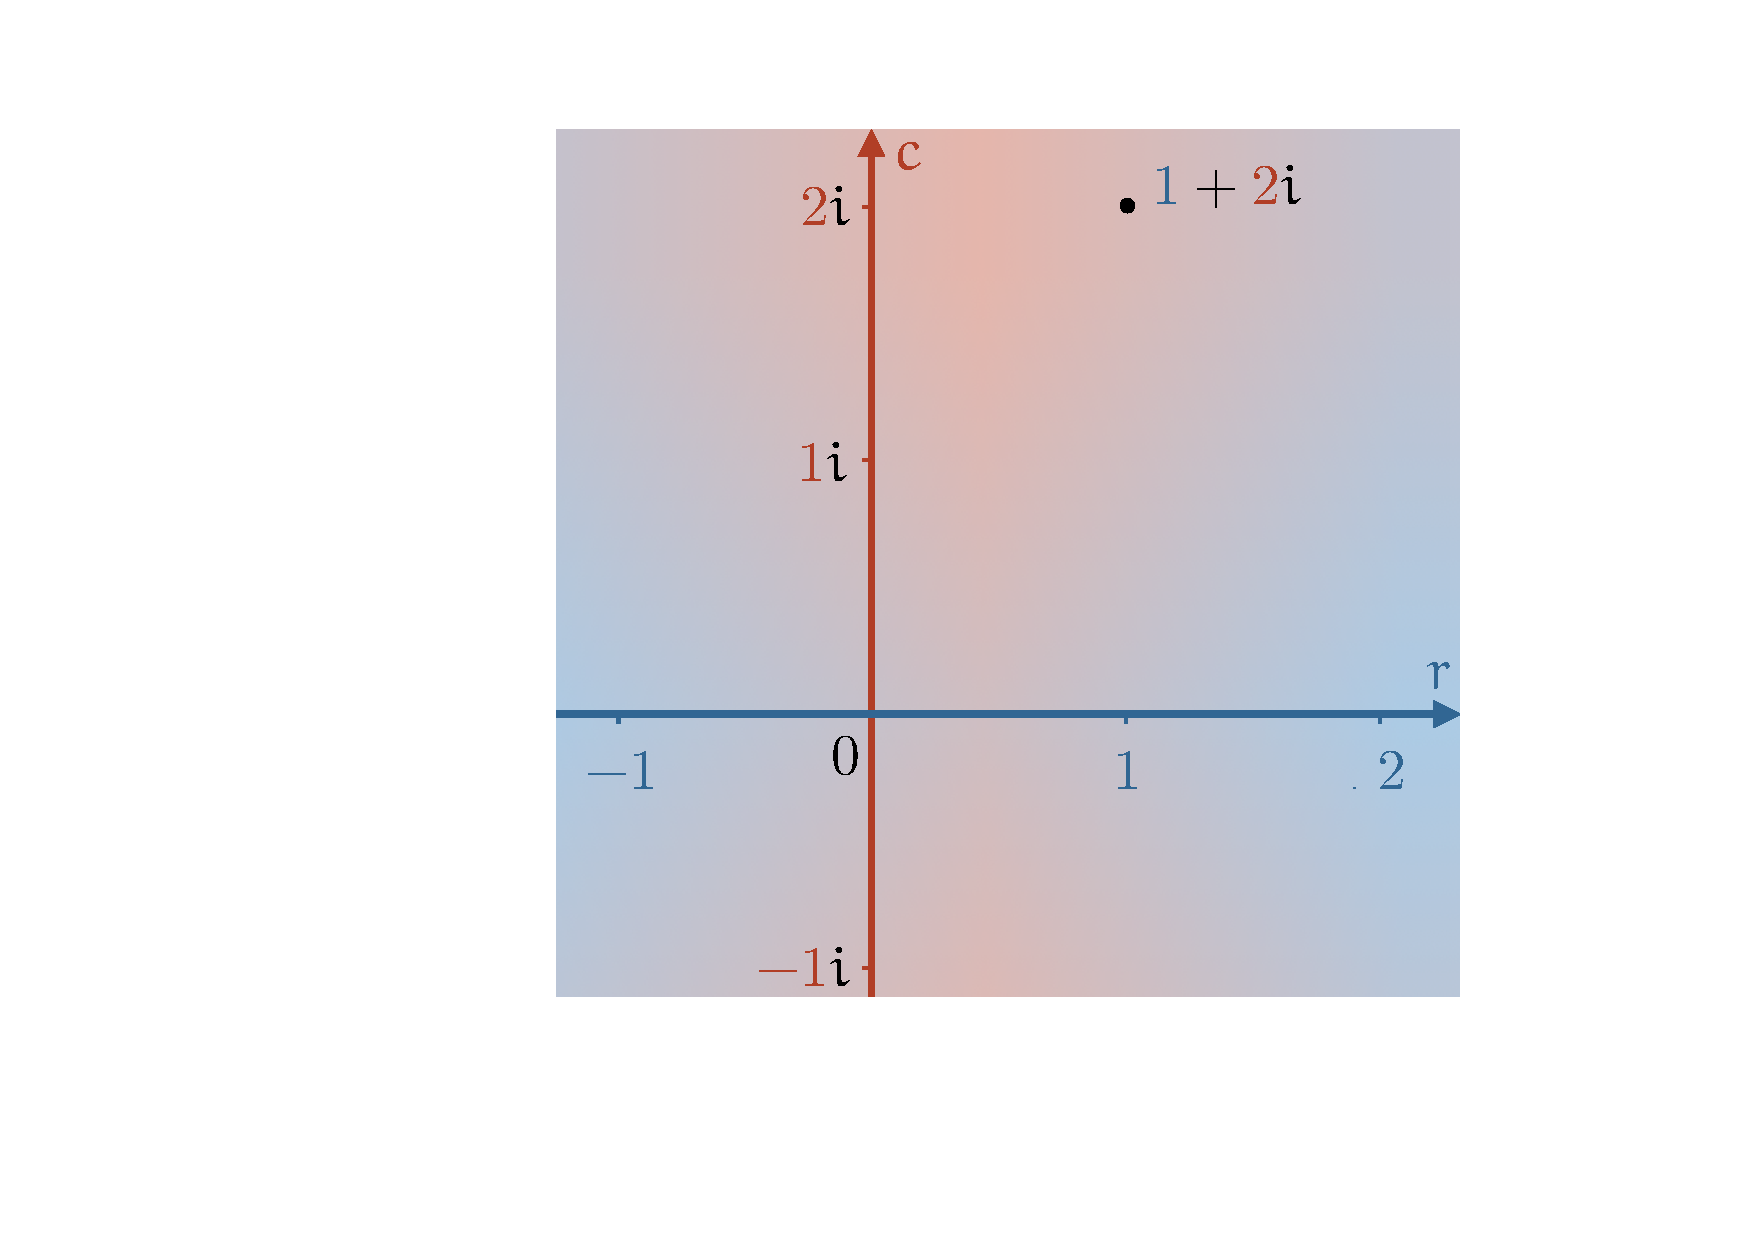
\includegraphics[width=0.7\textwidth]{./images/pca-3/complex-plane.pdf}
	}
\end{figure}

\index{Complex plane}

%<figure class="half center">
%<img src="/images/pca-3/complex-plane.svg">
%</figure>

The real-valued numbers that we already knew are a subset of the complex numbers: those complex number for which the \rc{imaginary part} is zero. In this picture, the real-valued numbers are on the \bc{horizontal axis}.

Note that this is just a visualization. There is nothing \emph{inherently} two-dimensional about the complex numbers, except that there is a very natural mapping from \(\mathbb C\) to \(\mathbb R^2\). At heart, it's just a set of numbers with a bunch of operations defined for them.

The nice thing about the mapping to the plane, however, is that we can take operations like multiplication, addition and so on, and see what they look like in this picture. This way, we can build a very helpful visual intuition for how the complex numbers behave.

Let's look at the most important concepts we'll need going forward. For addition, we can build on our existing intuitions. Adding two complex numbers works the same as adding two vectors in the plane: we place the tail of one on the head of the other.

\begin{figure}[H]
	\centerline{
		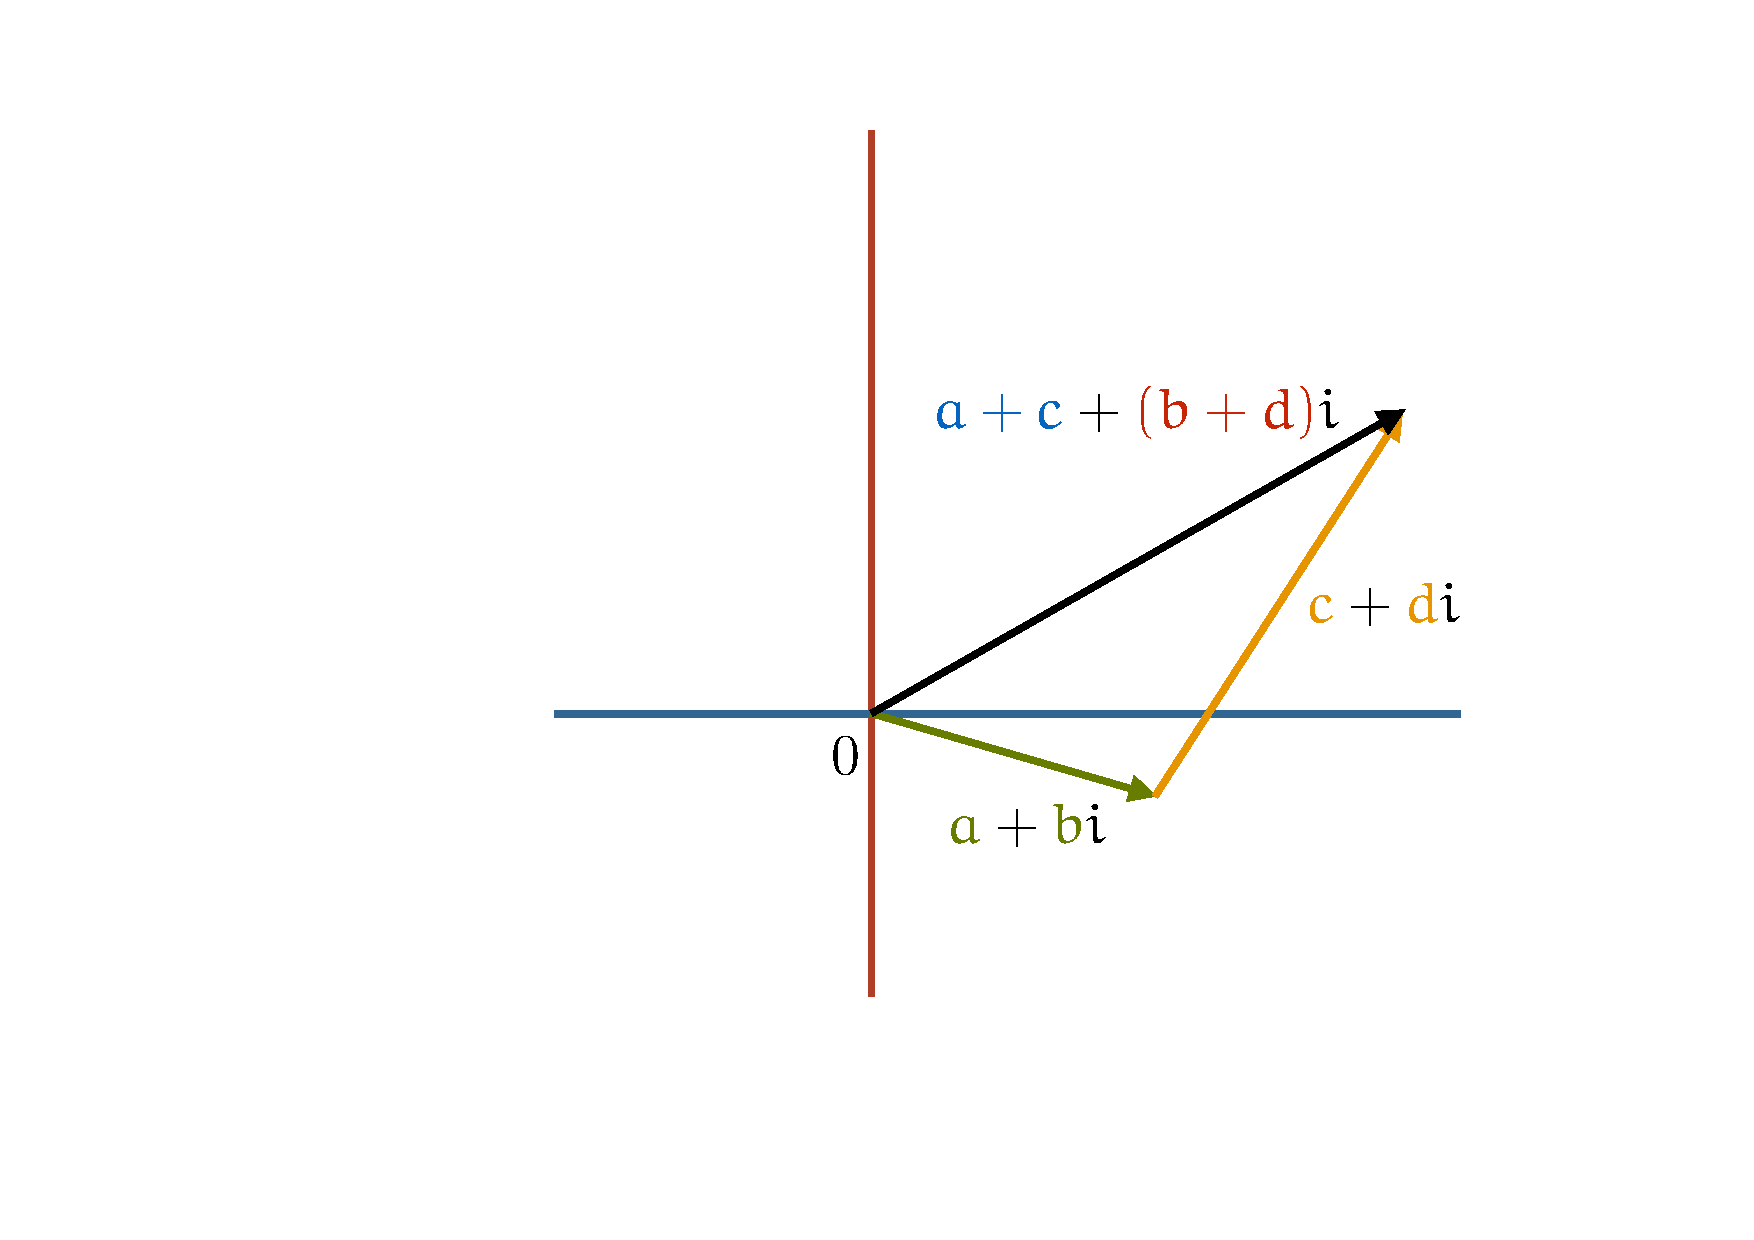
\includegraphics[width=0.7\textwidth]{./images/pca-3/addition.pdf}
	}
\end{figure}

%<figure class="half center">
%<img src="/images/pca-3/addition.svg">
%</figure>

The same logic shows that subtraction of complex numbers behaves as you'd expect. To compute \(x - y\), we subtract the real part of \(x\) from the real part of \(y\) and likewise for the imaginary part. Geometrically, this corresponds to vector subtraction in the plane.

\noindent To see what multiplication looks like, we can switch to a different way of representing complex numbers. Instead of giving the Cartesian coordinates \((\bc{r}, \rc{c})\) that lead to the number \(z = \bc{r} + \rc{c}i\), we use the \emph{polar} coordinates. We give an angle \(\gc{a}\) from the horizontal axis and a distance \(\gc{m}\) from the origin. The angle is also called the \emph{phase} and the distance is called the \emph{magnitude} or the \emph{modulus}. When we write a number like this, we'll use the notation \(z = \gc{m}\angle \gc{a}\). To refer to the magnitude of a complex number \(z\), which we'll be doing a lot, we use the notation \(|z|\).

\begin{figure}[H]
	\centerline{
		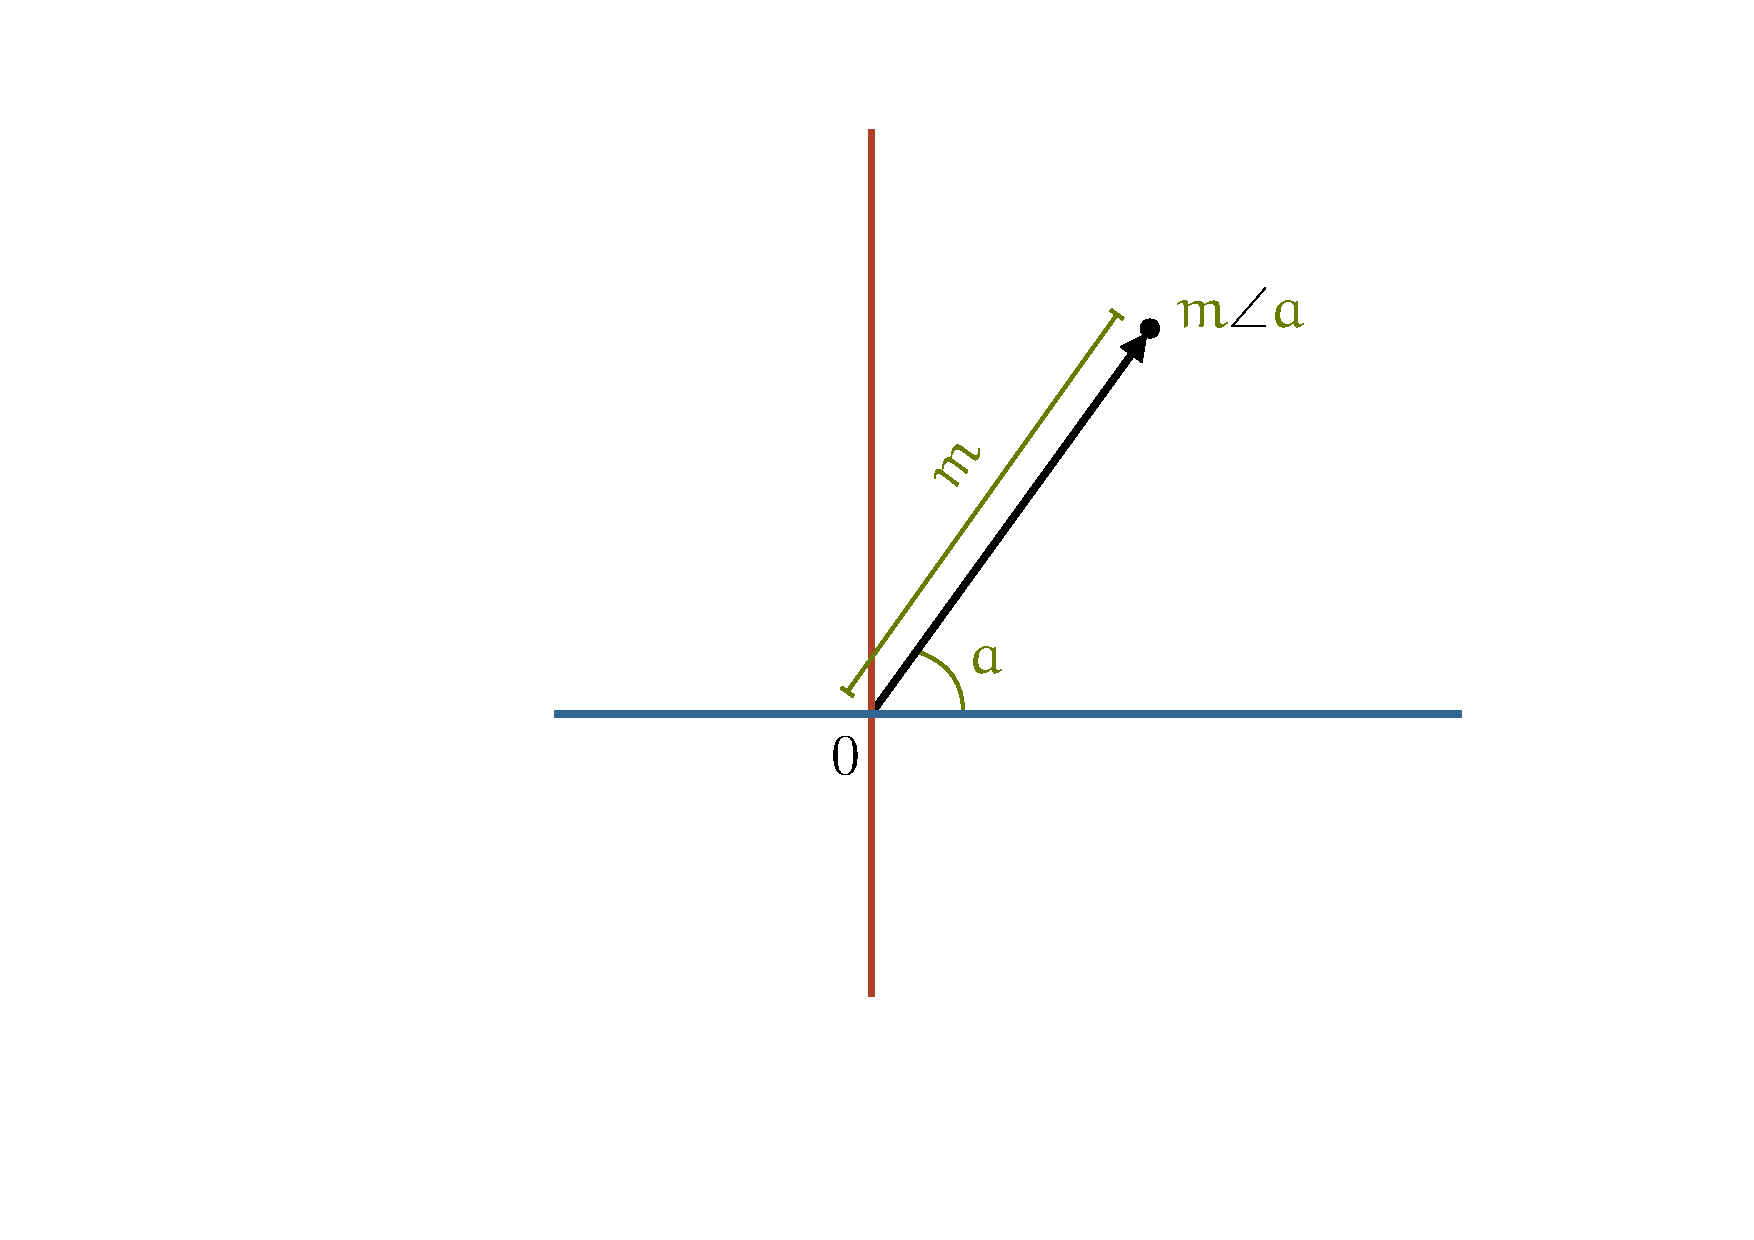
\includegraphics[width=0.7\textwidth]{./images/pca-3/polar.pdf}
	}
\end{figure}

%<figure class="half center">
%<img src="/images/pca-3/polar.svg">
%</figure>

 We call this representation of a complex number \emph{polar notation}, and the earlier representation \emph{Cartesian notation}.
 
 \index{Polar notation}\index{Cartesian notation}
 \index{Complex numbers!polar notation|textbf} \index{Complex numbers!Cartesian notation|textbf}

The reason polar notation is so useful, is that multiplication looks very natural in it. To see the relation, assume that we have a number \(z = \gc{m}\angle \gc{a}\). Then basic trigonometry tells us that in Cartesian notation, this number is written as \(z = \bc{\gc{m}\cos(\gc{a})} + \rc{\gc{m} \sin(\gc{a})} i\). 

\pagebreak
\noindent Let's see what happens if we take two numbers, in polar notation, and multiply them:

\begin{align*}
 & (\gc{m} \angle \gc{a})(\oc{n} \angle \oc{b})& \\
 &= (\gc{m}\cos(\gc{a}) + \gc{m} \sin(\gc{a}) i)\;(\oc{n}\cos(\oc{b}) + \oc{n}\sin(\oc{b}) i) \\
 &= \gc{m}\cos \gc{a} \;\oc{n} \cos \oc{b} + \gc{m} \sin \gc{a}\; \oc{n} \sin \oc{b} + (\gc{m} \cos \gc{a} \;\oc{n} \sin \oc{b}  + \oc{n}\cos \oc{b}\; \gc{m} \sin \gc{a})i \\
  &= \gc{m}\oc{n} (\cos \gc{a} \cos \oc{b} - \sin \gc{a} \sin \oc{b}) + \gc{m}\oc{n} (\cos \gc{a} \sin \oc{b} + \cos \oc{b} \sin \gc{a})i  \\
  &= \gc{m}\oc{n} \cos(\gc{a} + \oc{b}) + \gc{m}\oc{n} \sin(\gc{a} + \oc{b})i  \\
  &= (\gc{m}\oc{n}) \angle (\gc{a}+ \oc{b})
\end{align*}

In the third line, we apply the multiplication in Cartesian notation that we already worked out earlier. Then, in the fifth line, we apply some basic \href{https://en.wikipedia.org/wiki/List\_of\_trigonometric\_identities#Angle\_sum\_and\_difference\_identities}{trigonometric sum/difference identities}. 

What this tells us, is that when we view complex numbers in polar coordinates, multiplication has a very natural interpretation: the angle of the result is the \emph{sum} of the two original angles, while the magnitude of the result is the \emph{product} of the two original magnitudes.

\begin{figure}[H]
	\centerline{
		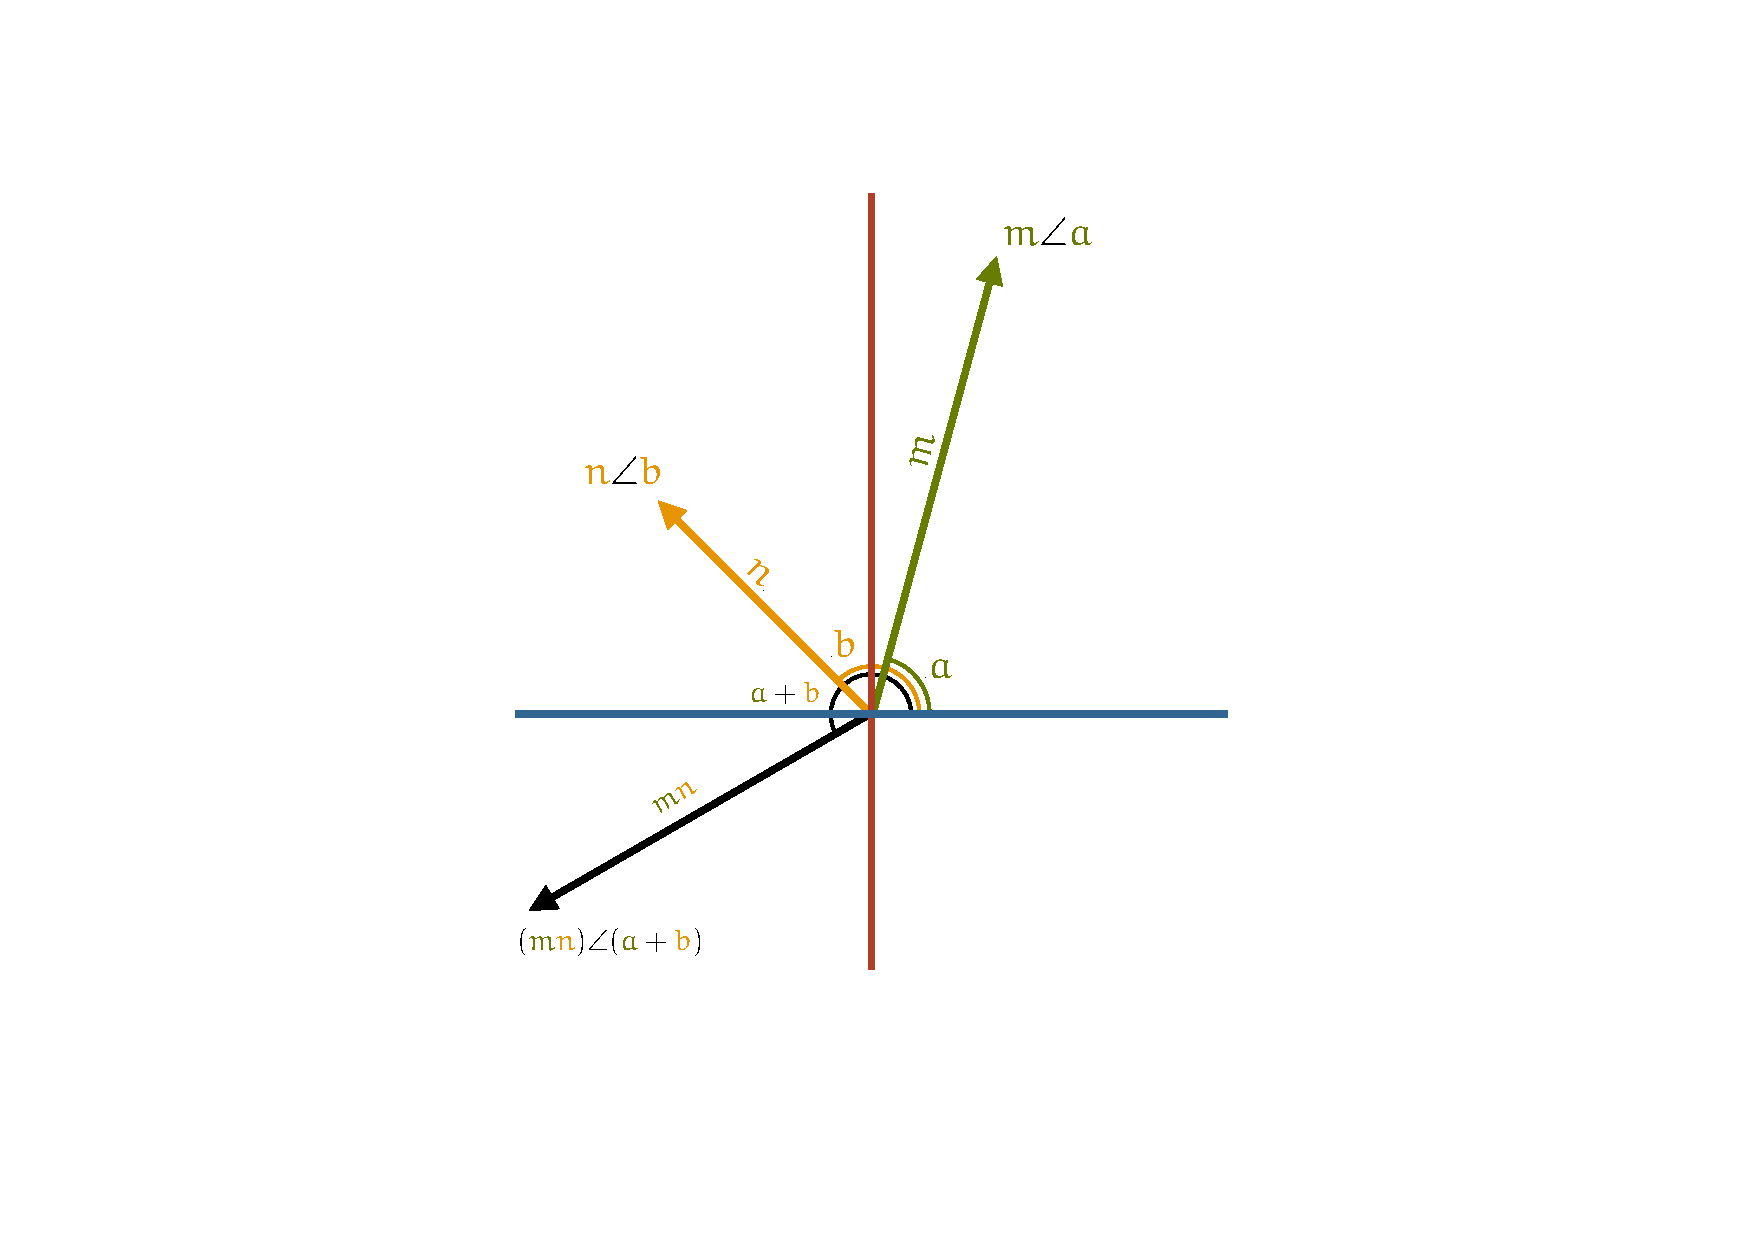
\includegraphics[width=0.7\textwidth]{./images/pca-3/multiplication.pdf}
	}
\end{figure}

%<figure class="half center">
%<img src="/images/pca-3/multiplication.svg">
%</figure>
%

The easiest way to define \emph{division} is as the operation that cancels out multipliciation. For each \(z\), there should be a \(z^{-1}\) so that multiplying by \(z\) and then by \(z^{-1}\) brings you back to where you were. Put simply \(zz^{-1} = 1\). Dividing by \(z\) can then be defined as multiplying by \(z^{-1}\). Using the polar notation, we can see that the following definition of \(z^{-1}\) does the trick:

\[z^{-1} = (\gc{m}\angle \gc{a})^{-1} = \frac{1}{\gc{m}}\angle -\gc{a} \p \]

Note how this view of multiplication agrees with special cases that we already know. For real numbers, the angle is always \(0\), and the magnitude is equal to the real value. Therefore, multiplying real numbers together reduces to the multiplication we already knew. 

The number \(i\) is written as \(1\angle90\deg\) in polar coordinates. That means that multiplying a number \(z\) by \(i\) keeps the magnitude of \(z\) the same, but rotates it by \(90\) degrees counter-clockwise. A real number multiplied by \(i\) is rotated from the \bc{horizontal} to the \rc{vertical} axis. If we multiply by \(i\) twice, we rotate \(180\) degrees, which for real numbers means negating them. This makes sense too, because \(z \cdot i \cdot i = z i^2 = z \cdot -1\).


\index{Complex numbers!exponentiation}

Which brings us to exponentiation. Raising complex numbers to arbitrary values, including to complex ones, is an important topic, but one which we can sidestep here. All we will need is the ability to raise a complex number to a natural number. That follows very naturally from multiplication:

\[
(\gc{m} \angle \gc{a})^n = (\gc{m} \angle \gc{a})(\gc{m} \angle \gc{a}) \ldots (\gc{m} \angle \gc{a}) = \gc{m}^n \angle n\gc{a} \p
\]

Again, let's look at some special cases. If the angle is \(0\), we stay on the real number line, and the operation reduces to ordinary exponentiation. If the magnitude is \(1\) but the angle is nonzero, then we rotate about the origin over the unit circle in \(n\) steps of angle \(\gc{a}\).

\begin{figure}[H]
	\centerline{
		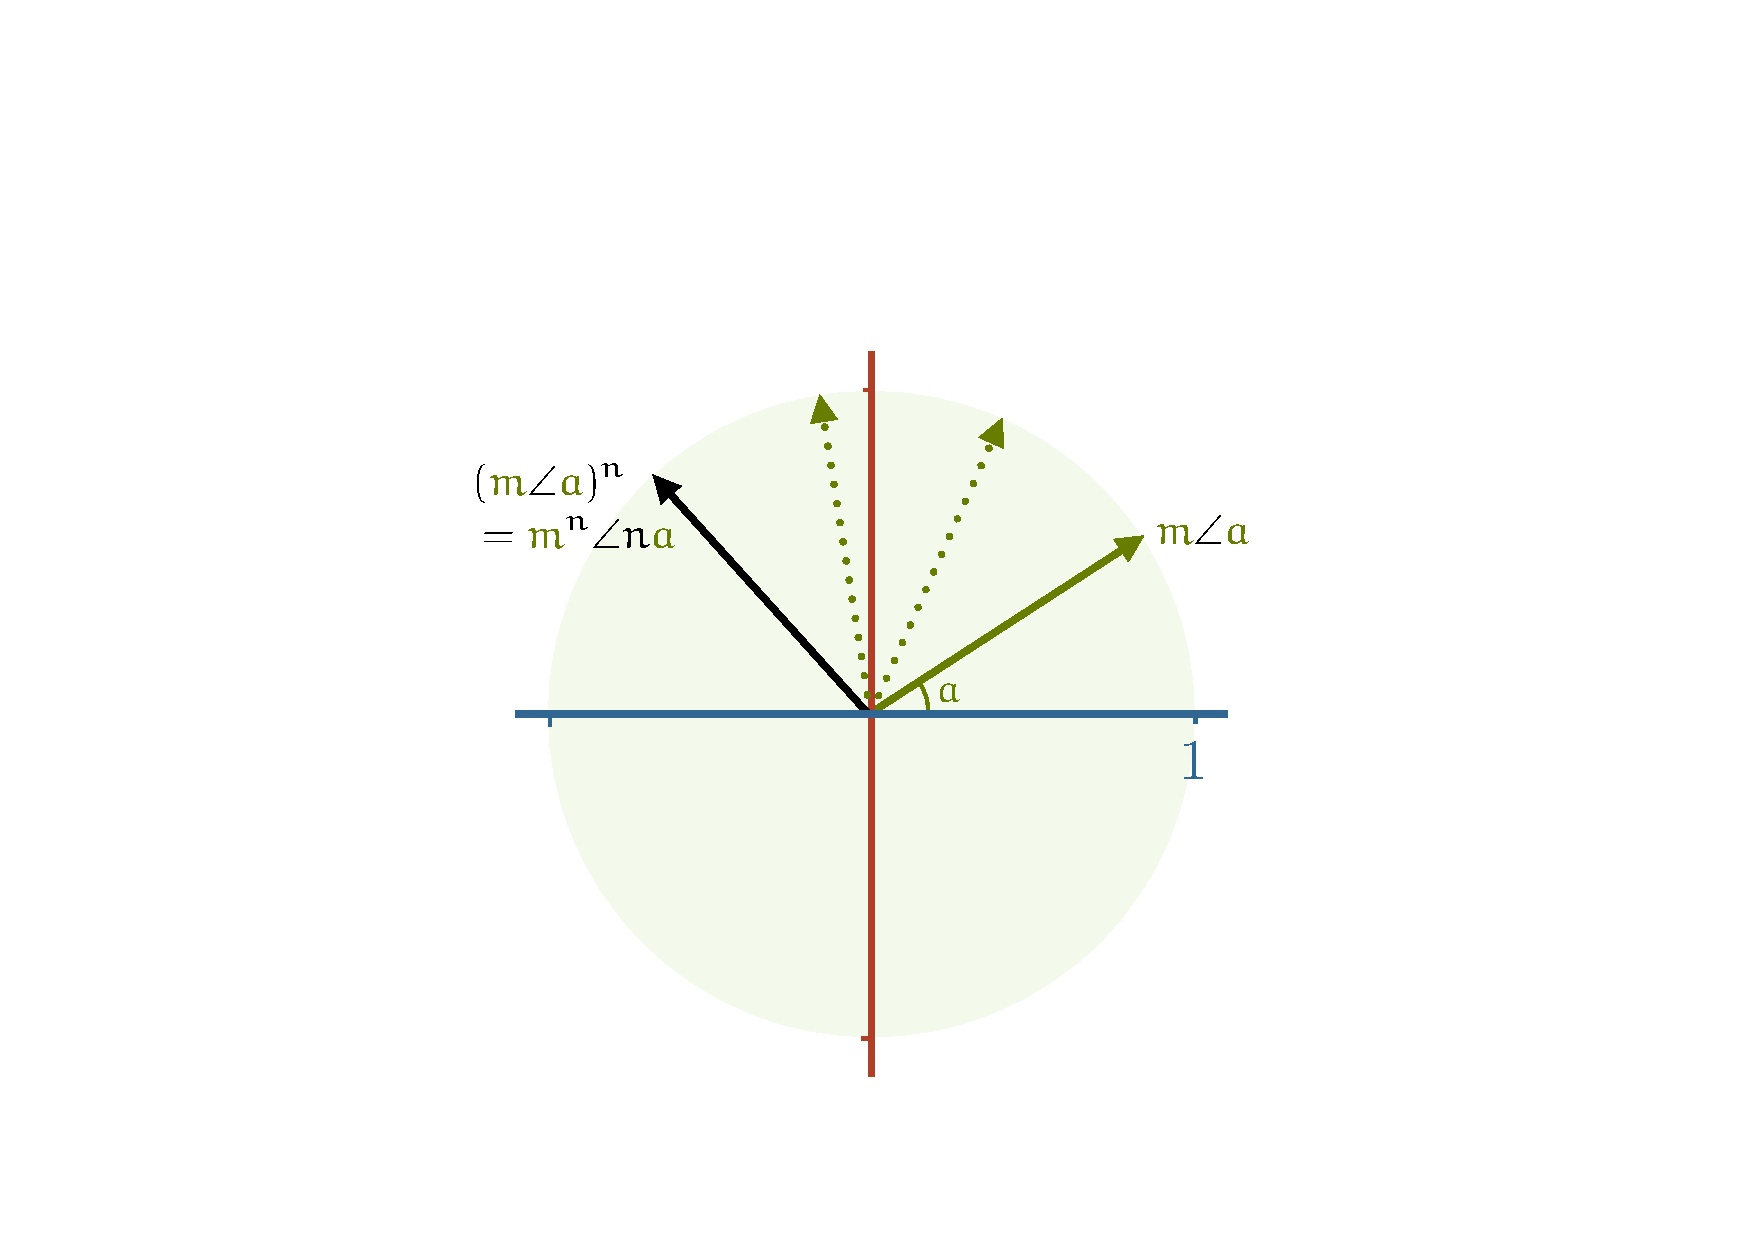
\includegraphics[width=0.7\textwidth]{./images/pca-3/exponentiation.pdf}
	}
\end{figure}

%<figure class="half center">
%<img src="/images/pca-3/exponentiation.svg">
%<figcaption>Exponentiation with unit magnitude.
%</figcaption>
%</figure>

The main thing we need, however, is not integer exponentiation, but its inverse: the \(n\)-th root. Given some complex number \(z = m\angle a\), which other number do we raise to the power \(n\) so that we end up at \(z\)? The answer follows directly from our polar view of the complex plane: the magnitude should be \(\sqrt[n]{m}\), which is just the real-valued \(n\)-th root, and the angle should be \(a/n\).

Let's check for \(\sqrt{-1}\), which started all this business. Which number should we raise to the power 2, so that we get \(-1\)? The magnitude of \(-1\) is \(1\), so our number has magnitude \(\sqrt{1} = 1\). Now we need a number with magnitude one, so that twice its angle equals \(180 \degree\). This is a \(90 \degree\) angle, so our number is \(1\angle 90\degree\), which is exactly where we find \(i\).

Notice how this solves the problem we had when we were constrained to the real line. Then we had negative numbers to deal with, and the real \(n\)-th root does not exist for negative numbers. Now, we are only ever applying the \(n\)-th root to \emph{magnitudes}, which are positive. The rest is dealt with by rotating away from the real numbers. This means that when it comes to complex numbers, we can always find some number that, when raised to \(n\), gives us \(z\). We call this the complex \(n\)-th root \(\sqrt[n]{z}\).

Note however, that this is not always a \emph{unique} number. Let's say we raise \(1\angle 10\degree\) to the power of \(4\). This gives us \(1\angle 40\degree\), so \(1\angle 10\degree\) is a fourth root of \(1\angle 40\degree\). However, if we raise \(1\angle 92.5\degree\) to the power of \(4\), we get \(1\angle 370\degree\), which is equal to \(1\angle 10\degree\) as well. Any angle \(a'\) for which \(a'\frac{1}{n}\,\text{mod}\;360 = a\) will give us an \(n\)-th root of \(m\angle a\). 

How many solutions does this give us for any given number? It's easiest to visualize this if we plot the \(n\)-th roots of 1.

\begin{figure}[H]
	\centerline{
		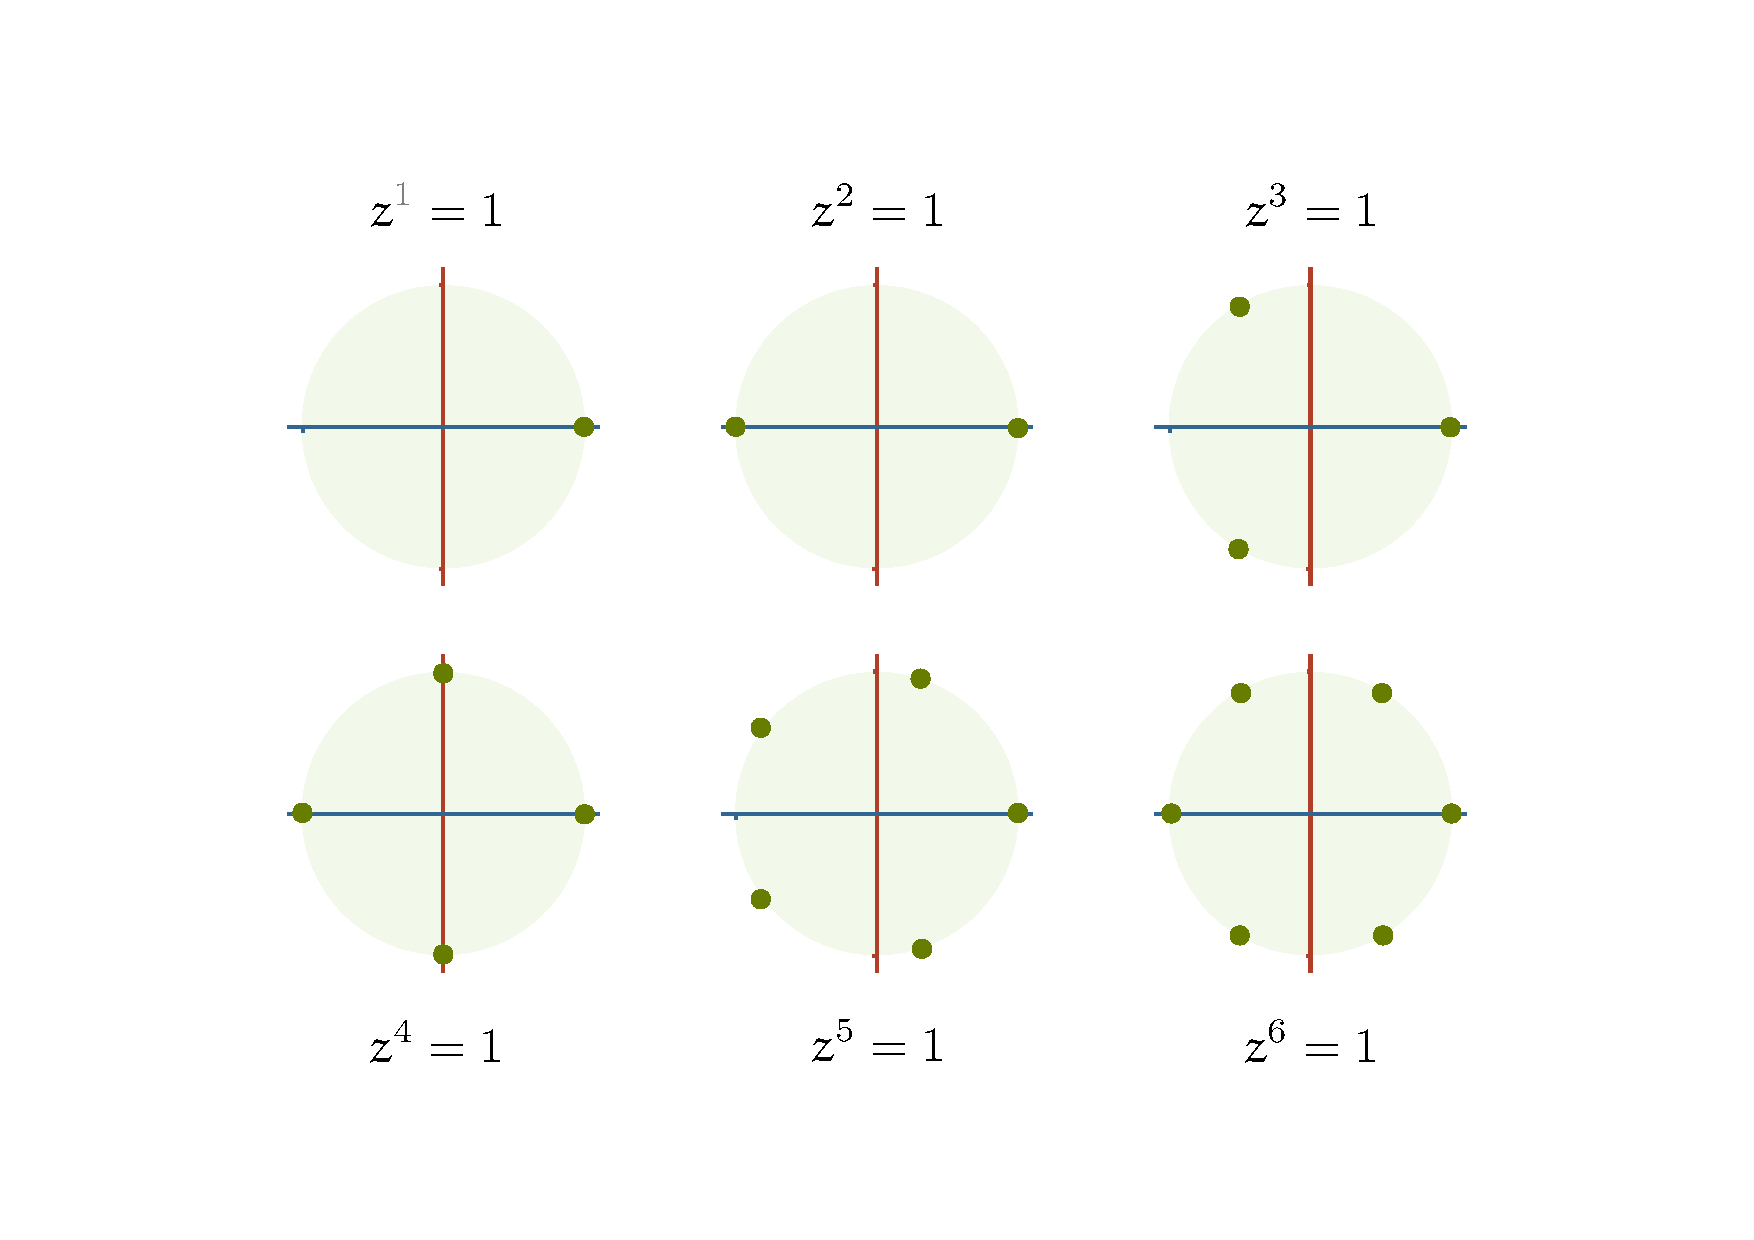
\includegraphics[width=1\textwidth]{./images/pca-3/nth-roots.pdf}
	}
\end{figure}

%<figure class="narrow">
%<img src="/images/pca-3/nth-roots.svg">
%</figure>

For each, of course, the real value \(1\) is a solution, but for the higher powers, there are additional solutions on the unit circle. For \(\sqrt[2]{1}\), for instance, multiplying \(-1\) by itself rotates it by 180 degrees to coincide with \(1\). For \(\sqrt[3]{1}\), we get three roots, two of which are non-real. The solution with angle \(120\deg\), when raised to the power of \(3\) gives us an angle of \(360\deg = 0\deg\). The solution with angle \(240\deg\) puts the angle after cubing at \(720 \deg = 0 \deg\). 

In short, every multiple of \(360\): \(0\), \(360\), \(720\), \(1080\), \(\ldots\), can be divided by \(n\) to give us a solution. Once we get to \(360n\), dividing by \(n\) gets us back to a solution we've already seen, so we get \(n\) unique solutions in total.

To translate this to roots of any complex number \(m\angle a\), we simply scale the circle so that its radius is \(\sqrt[n]{m}\) and then rotate it so that the first solution points in the direction of \(a/n\).

\begin{figure}[H]
	\centerline{
		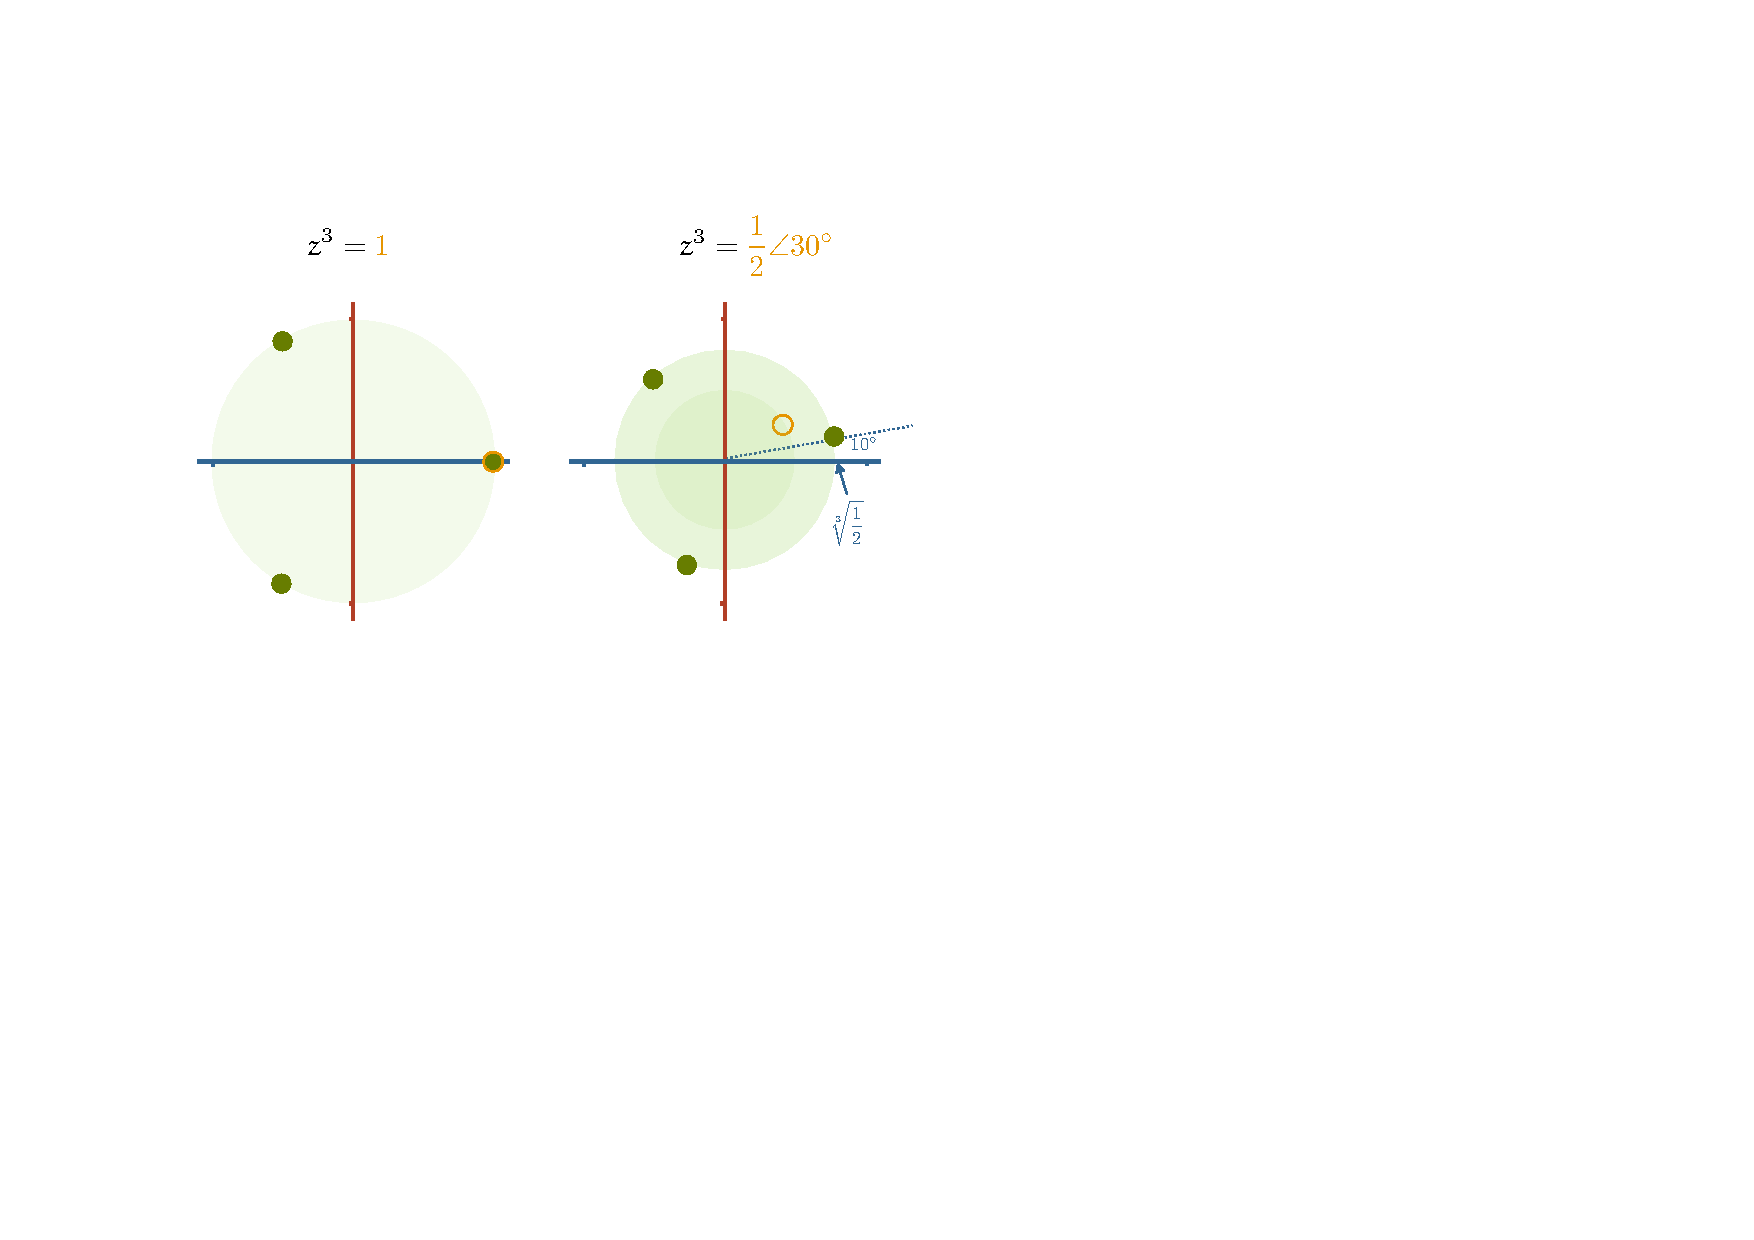
\includegraphics[width=1.05\textwidth]{./images/pca-3/general-root.pdf}
	}
\end{figure}

%<figure class="narrow">
%<img src="/images/pca-3/general-root.svg">
%</figure>

\section{The fundamental theorem of algebra}

The reason we are bringing in complex numbers, is that we are interested in talking, in general terms, about the roots of the chracteristic polynomial. When all we have access to are real-valued numbers, this becomes a messy and unpredictable business. A polynomial of order \(n\) can have anywhere between 0 and \(n\) roots. When we add complex numbers to our toolbelt, the whole picture becomes a lot simpler. And that is down to a result called \emph{the fundamental theorem of algebra}.

\index{Roots!of the characteristic polynomial}

The theorem has many equivalent statements, but this is the one most directly relevant to our purposes.

\begin{theorem}[The fundamental theorem of algebra] Any non-constant polynomial of order \(n\) has exactly \(n\) complex roots, counting multiplicities.
\end{theorem}

\index{Fundamental theorem of algebra|textbf}\index{Multiplicities}

\begin{aside}%
For now, don't worry about what is meant by multiplicities. We'll dig into that later. A constant polynomial is a function like \(f(x) = 3\), which will not have any roots.
\end{aside}

To prove this theorem, the first thing we need is to show that each such polynomial has \emph{one root}. After that, the rest is straightforward. So straightforward (to some) that this is often seen as an alternative statement of the fundamental theorem:

\begin{theorem}[\hspace{-0.15em}The fundamental theorem of  algebra (variant)] Any non-constant polynomial of order \(n\) has at least one complex root.
\end{theorem}

%<!-- 
%
%We'll first show that this holds for a subset of polynomials, which we'll call <em>simple polynomials</em>. That is, any polynomial of the form 
%
%\[
%p(z) = \bc{a}(z - \bc{b})^k + \bc{c}
%\]
%
%where \(k\) is a positive integer and \(\bc{a}\), \(\bc{b}\) and \(\bc{c}\) are arbitrary complex numbers, with \(\bc{a}\) non-zero.
%
%<div class="theorem"><strong class="gc">Lemma</strong> Any simple polynomial has at least one complex root.
%</div>
%<div class="proof"><p><em>Proof.</em> By simple algebraic manipulation, we get:
%\[\begin{align*}
% \bc{a}(z - \bc{b})^k + \bc{c} & = 0 \\
% z & = \sqrt[k]{-\frac{\bc{c}}{\bc{a}}} + \bc{b} \p
%\end{align*}\]
%This requires the operations of division, multiplication, addition and root taking. 
%
%We showed above that each of these always leads to another complex number (the complex numbers are <em>closed</em> under these operations), so the solution must exist in \(\mathbb C\).
%<span class="qed" /></p></div>
%
%The idea that we can take any integer root of any complex number is the fundamental building block of the theorem. From that, all we have to to is extend the idea to all polynomials. We do that by showing that locally, any polynomial can be well approximated by a simple polynomial. 
%-->

Let
\[
p(z) =\bc{c_n}z^n + \ldots + \bc{c_1}z + \bc{c_0}
\]

be our polynomial. For our purposes, we can think of the coefficients as real-valued, but the theorem holds for complex coefficients as well. The argument \(z\) and the result \(p(z)\) can always be complex.

To find a root of \(p\), we will consider the function \( |p(z)| \). That is, the magnitude of the complex number that we get out of \(p\). This provides the following benefits:

\index{Magnitude function}

\begin{itemize}
\item The magnitude is always non-negative. That means that the lowest possible value that \(|p(z)|\) can take on is \(0\), at which point we must have \(p(z) = 0\). In short, for a root of \(p(z)\), \(|p(z)|\) is both \(0\) and at a minimum.
\item Since the magnitude of a complex number is a single real value, \(|p(x)|\) is a function from two dimensions (the complex plane) to one dimension (the reals) and we can easily visualize it in three dimensions. This is not so easy for \(p(x)\) itself, since we have a two-dimensional input \emph{and} a two-dimensional output.
\end{itemize}

%<!-- 
%
%Our big shortcut in this proof will be to look at what this polynomial does in the extreme cases: when its input is very far from 0, and when it's input is very close to zero. Let's start by looking at real-valued polynomials of the from \(x^n\). Consider the following plot.
%
%What we see is that if \(x\) is larger than 0 \(x^3\) grows much quicker than \(x^2\). The distance between them \(x^3 - x^2\) clearly grows unbounded: if you give me any number \(b\), I can give you a number \(x\) for which the difference between the two is larger than \(b\). This means that in a real valued polynomial of degree \(n\), the \(x^n\) term <em>dominates</em>. For large enough inputs, it's bigger than all the other terms put together. At that point, we know that if \(\bc{c_n}x^n\) is bigger than \(0\), so is \(p(x)\).
%
% - diagram
%
%The same holds for complex-valued polynomials. Here, each term is essentially a vector in the complex plane, all of which we're adding together. The magnitude of each of these vectors is the magnitude of the input raised to some power. The influence of the highest-degree term is kept down the most if all the other terms have vectors pointing in the exact opposite direction to it. This puts all vectors on one line, which bring us back to the previous diagram.
%
% - diagram
% 
% -->

Our big shortcut in this proof will be to look at what the magnitude does in extreme cases: for very large inputs, and for inputs very close to the minimum. We will see that in both cases, the function can be approximated well by the magnitude of a simple polynomial. 

To see this, let's start with a simple real-valued example. The polynomial \(p(x) = \rc{x^3} + \bc{x^2} + \gc{x}\) in the positive range. In this area, \(p(x)\) is equal to its magnitude, so we don't need to worry about the distinction yet.

\vspace{-1em}
\begin{figure}[H]
	\centerline{
		\includesvg[width=1\textwidth]{./images/pca-3/real-polynomialmedium.svg}
	}
\end{figure}
\vspace{-1em}

%<figure class="narrow">
%<img src="/images/pca-3/real-polynomialmedium.svg">
%</figure>

\noindent What we see here, is that as \(x\) gets bigger, the term \(\rc{x^3}\) dominates. Almost all the contribution to the magnitude comes from this term, and pretty soon, the simpler polynomial \(\rc{x^3}\) becomes a pretty good approximation of the polynomial \(\rc{x^3} + \oc{x^2} + \bc{x}\). This is not surprising, since \rc{the cube} grows much faster than \oc{the square} which grows much faster than \bc{the identity}.

Toward \(x=0\), where \(p\) has a minimum, the opposite happens. As \(\rc{x^3}\) grows the fastest when \(x > 1\), so it \emph{shrinks} the fastest when \(0 < x < 1\). In this regime the term that shrinks the slowest, \(\bc{x}\) begins to dominate, and \(\bc{x}\) becomes a good approximation of the function \(p\).

\enlargethispage{3em}

Of course, this is just one polynomial. If we move to complex polynomials, and we allow for any order and all possible coefficients, does this pattern still hold? Let's imagine a generic complex polynomial. In this case, all terms in the polynomial are complex numbers, and the value of the polynomial is their sum.

\vspace{-1em}
\begin{figure}[H]
	\centerline{
		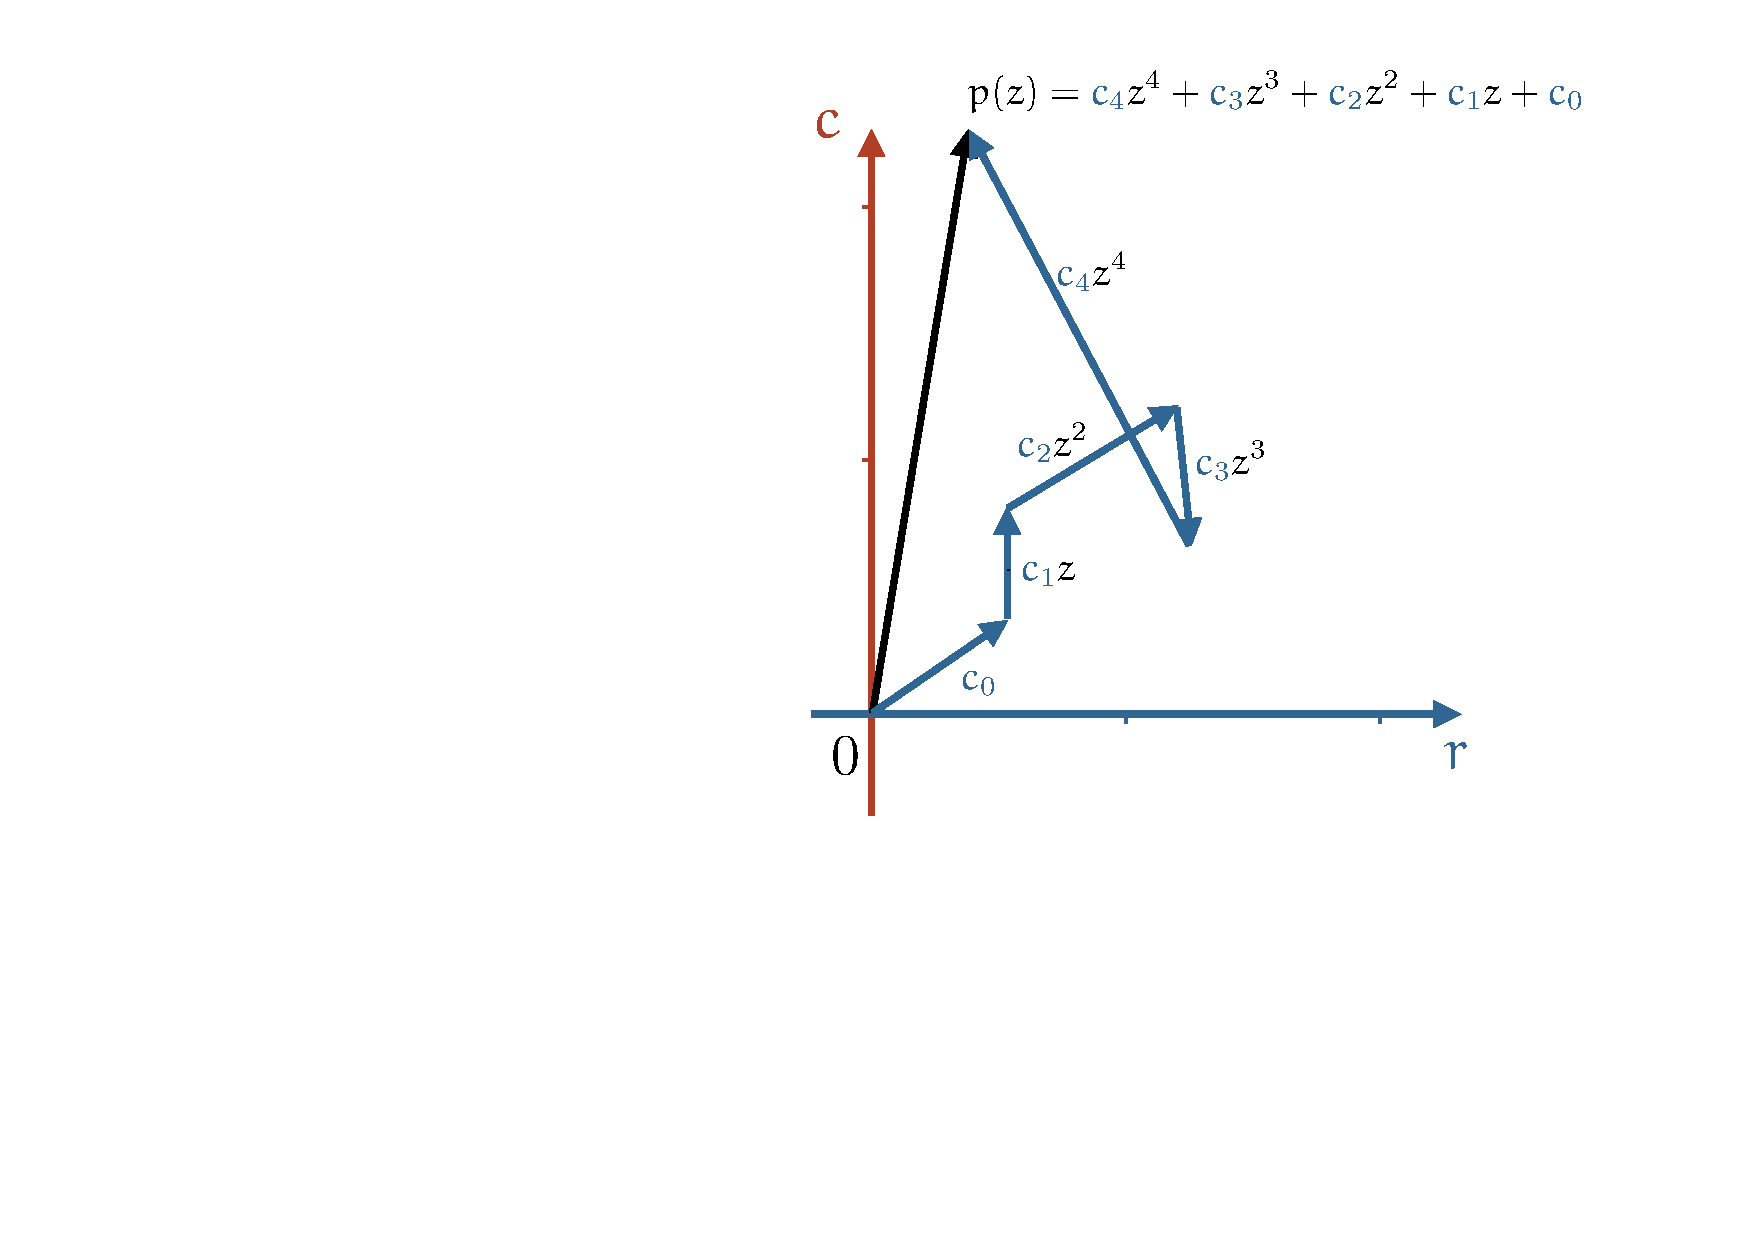
\includegraphics[width=0.6\textwidth]{./images/pca-3/polynomial-terms.pdf}
	}
\end{figure}
\vspace{-1em}

\index{Dominant terms of a polynomial}\index{Polynomial!dominant terms of}

%<figure class="tile4 centering">
%<img src="/images/pca-3/polynomial-terms.svg">
%</figure>

\noindent The magnitude \(|p(z)|\) of the polynomial at \(z\) is the distance of the end result to the origin. Each term contributes to this magnitude in a different direction. If we want to show that a particular term dominates, we can look at the worst case: that term points in one direction, and all other terms point in the exact opposite direction.

\begin{figure}[H]
	\centerline{
		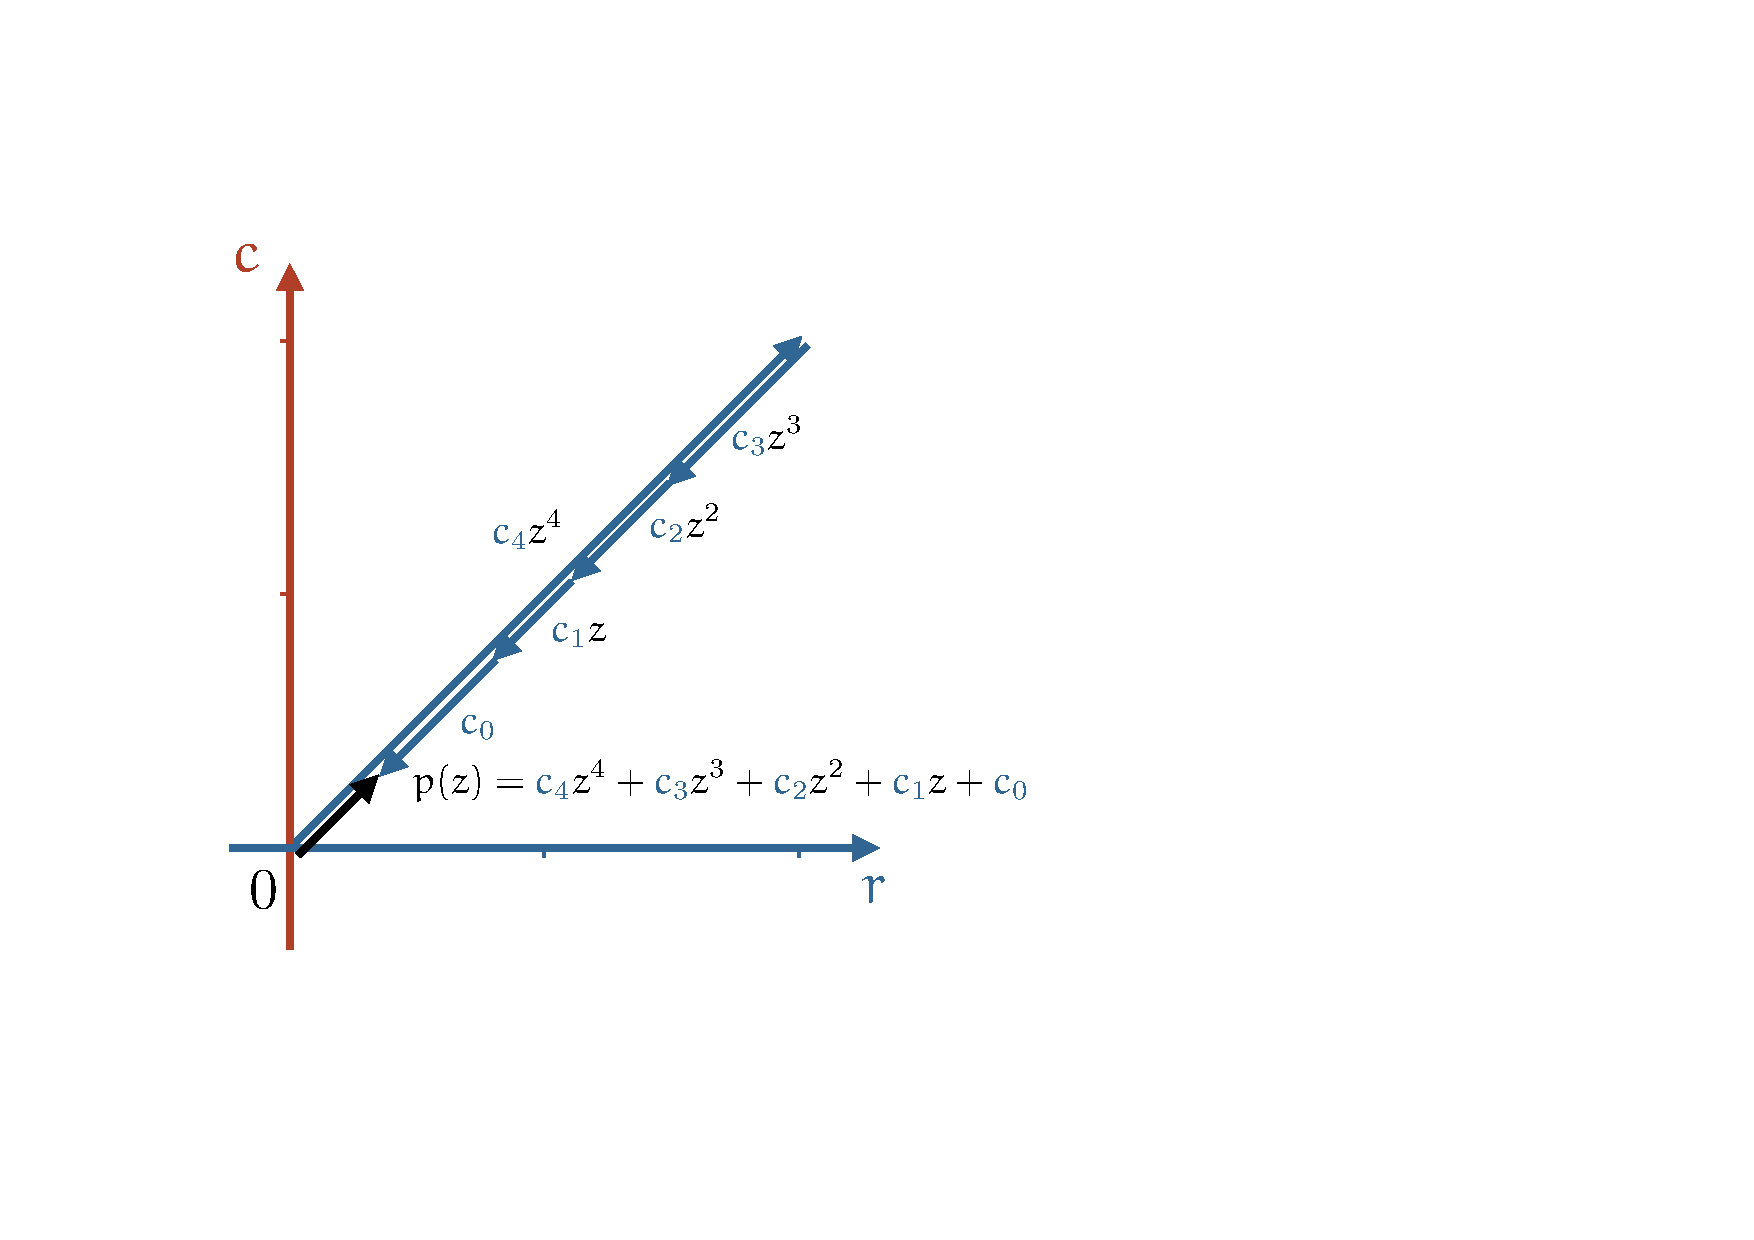
\includegraphics[width=0.6\textwidth]{./images/pca-3/term-domination.pdf}
	}
\end{figure}

%<figure class="tile4 centering">
%<img src="/images/pca-3/term-domination.svg" class="third">
%<figcaption>To show that the term \(\bc{c_4}z^4\) dominates, we can assume that all other terms point in the opposite direction. If the remainder of this term minus the others is still close to the magnitude of \(p(z)\), this will also be true when the other terms point in other directions.</figcaption>
%</figure>

In this case, we can ignore the angles of the terms and focus only on their magnitudes. If we assume the highest-order term points in the opposite direction of the rest, the total magnitude is

\begin{align*}
|p(z)| &= \left |\bc{c_{n}} {z}^n\right| - \left|\bc{c_{n-1}} {z}^{n-1}\right | - \ldots - \left |\bc{c_{1}} z\right | - \left |\bc{c_{0}}\right| \\
& = |\bc{c_{n}}| {|z|}^n - |\bc{c_{n-1}}| {|z|}^{n-1} - \ldots - |\bc{c_{1}}| |z| - |\bc{c_{0}}|
\end{align*}

\begin{aside}Note that the terms we are subtracting are all magnitudes, so they are all positive.\end{aside}

We will first use this to show that \(|p(z)|\) has some definite minimum. One alternative situation would be if \(p(z)\) is a function that is positive everywhere and monotonically increasing in some direction, like \(e^x\) is on the real number line. We'll need to exclude such possibilities first.

Assume that \(|z| > 1\) for some \(z\). If so, we make the total value of the sum \emph{smaller} if we replace all lower-order powers by \(z^{n-1}\). This means that

\begin{align*}
|p(z)| &> |\bc{c_{n}}| {|z|}^n  - |\bc{c_{0}}| - \sum_{i\in 1..n-1} |\bc{c_{i}}| {|z|}^{n-1} \\
 &= |\bc{c_{n}}| {|z|}^n - |\bc{c_{0}}| - {|z|}^{n-1}\sum_{i\in 1..n-1} |\bc{c_{i}}| \\
 &= {|z|}^{n-1} \left (|\bc{c_n}| {|z|} - \sum_{i\in 1..n-1} |\bc{c_{i}}|\right) - |\bc{c_0}|
\end{align*}

If we choose \(z\) so that its magnitude is larger than \(\frac{1}{|\bc{c_n}|} \sum_i |\bc{c_i}|\), the factor in brackets becomes positive. Beyond that, we know that there is some value of \(|z|\) large enough that the first term is bigger than the second. In short, for a suffciently large \(B\), we can always choose a value of \(z\) such that \(|p(z)|\) is larger than \(B\).

This means we can draw some large circle with radius \(R\), find the smallest value of \(|p(z)|\) inside the circle, and then draw a second circle with radius \(B\) so that all values outside of \(p(z)\) outside the second circle are larger than this minimum inside the first circle. This means \(|p(x)|\) has a definite minimum inside the second circle.

Now, all we need to do is show that this minimum can be expressed by a complex number. To do that, we'll follow the same sort of argument, but with the magnitude going to \(0\), so that the \emph{lower-order} terms dominate.

First, let \(z_0\) be the minimum we've just shown must exist. Translate \(p\) so that this minimum coincides with the origin, and call the result \(q(z)\). Specifically, \(q(z) = p(z - z_0)\).

This is another \(n\)-th order polynomial. We'll call its coefficients \(\bc{d_i}\). Note that \(q(0)\) has the same value as \(p(z_0)\) by construction. What we want to show is that \(p(z_0) = 0\).

In many polynomials the lowest-order term is the first-order term \(\bc{c_1}z\). However, we need to account for cases where this term is always zero. To be general, we write \(q\) as
%
\[
q(z) = \bc{d_0} + \bc{d_k}z^k + \bc{d_{k+1}}z^{k+1} + \;\ldots\; + \bc{d_n}z^n
\]

where \(k\) is the order of the lowest-order, non-constant term.

\noindent We'll show that the proportion of the sum contributed by the higher order terms vanishes as we get near zero, so we can take the simpler function \(q'(z) = \bc{c_0} + \bc{c_k}z^k\) as a good approximation, that becomes perfect at the origin.

\begin{aside}
Note that \(q(0) = q'(0)\).
\end{aside}

More formally, lets look at the ratio between the higher-order terms and the \(k\)th-order term:

\[
r = \frac{  |\bc{d_{k+1}}||z|^{k+1} + \;\ldots\; + |\bc{d_n}||z|^n  }{  |\bc{d_{k}}||z|^k } \p
\]

Assuming that \(|z| < 1\), the numerator is made bigger by reducing all exponents to \(z^{k+1}\), so 

\[
r < \frac{  |z|^{k+1} \sum_{i\in k+1..n} |\bc{d_i}| }{  |\bc{d_{k}}||z|^k } = |z|\frac{   \sum_{i} |\bc{d_i}| }{  |\bc{d_{k}}| } \p
\]

The second factor is a constant, so if we want to make the contribution of the higher order terms less than some given \(\epsilon\), we just need to choose a \(z\) with small enough magnitude.

\begin{aside}Specifically \(|z| < \epsilon \frac{ |\bc{d_k}| }{ \sum_i |\bc{d_i}|}\). Fill this into the above, and note that the two fractions cancel out, leaving only \(\epsilon\).
\end{aside}

This allows us to continue our analysis with \(q'\) instead of \(q\). Next, we can show that because \(|q'(z)|\) has a minimum at \(0\), that minimum must be equal to \(0\), so that \(\bc{d_0} = 0\).

At first, this may not be obvious. Why should a function \(q'(z) = \bc{c_k}z^k + \bc{c_0}\) necessarily have \(\bc{c_0} = 0\) if its magnitude has a minimum at \(0\)? It becomes clearer if we take the image of the roots of \(z^n -  1\) that we showed earlier, and create a 3d plot of the corresponding magnitude functions \(|z^n - 1|\).

\begin{figure}[H]
	\centerline{
		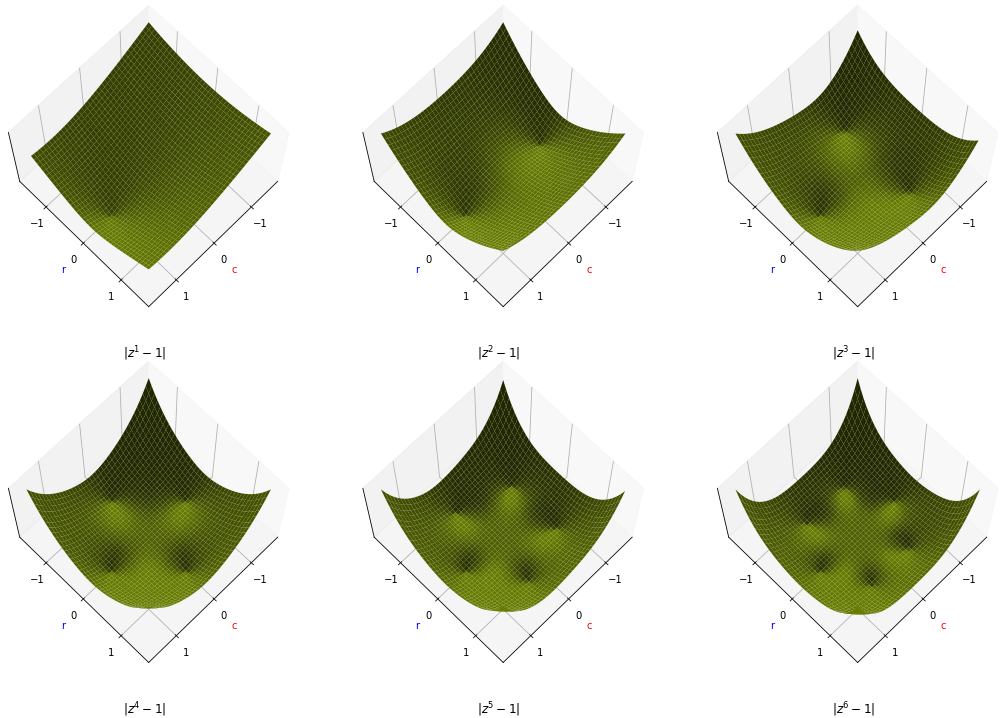
\includegraphics[width=1.1\textwidth]{./images/pca-3/roots-3d.png}
	}
\end{figure}

%<figure class="wide centering">
%<img src="/images/pca-3/roots-3d.png" class="three-quarters">
%</figure>

This kind of picture applies to the more general function \(|\bc{c_k}z^k + \bc{c_0}|\) as well: the two constants rotate the image and change how close the roots are to the origin, but unless \(\bc{c_0} = 0\), we get a ring of roots some distance from the origin and no root at the origin. This contradicts what we know: that \(|q(z)|\) has a minimum at 0, so we know that \(c_0\) must be \(0\).

To prove this formally, let \(z = \sqrt[k]{-\bc{d_0}/\bc{d_k}}\), one of the roots of \(q'\) , and let \(\epsilon\) be some real value near 0. Then we have:

\begin{align*}
|q'(\epsilon z)| &= |\bc{d_0} + \bc{d_k} \cdot - \epsilon^k \frac{\bc{d_0}}{\bc{d_k}}|  \\
&= |\bc{d_0} - \epsilon^k \bc{d_0}|
\end{align*}

Note that both terms in this last line point in the same direction, so if \(\bc{d_0} >0\), the resulting magnitude is smaller than \(|\bc{d_0}|\), which contradicts what we already know: that \(|\bc{d_0}|\) is the minimum of \(q'\). Therefore \(\bc{d_0} = 0\), \(q(0)\) is a root of \(q\) and \(p(z_0)\) is a root of \(p\).

\begin{aside}It's instructive to look over this proof, and try to figure out why the same argument wouldn't work for real-valued polynomials. 

The answer is in the step where we chose \(z = \sqrt[k]{-\epsilon\bc{d_0}/\bc{d_k}}\). This allowed us to approach the origin from one of the roots of \(\bc{c_k}z^k + \bc{c_0}\), and to observe that the magnitude increases. In the real-valued world, we cannot always make this choice, because the root may be of a negative number.  
\end{aside}
 
\subsection{From one root to \(n\) roots}

Now that we know that each polynomial has at least one root, how do we get to multiple roots? In high school, we learned that when we were faced with a (real valued) second-degree polynomial to solve, sometimes, if we were lucky, we could find its factors. For instance, the function:

\[
f(x) = x^2 - \bc{3}x + \bc{2}
\]

can be rewritten as

\[
f(x) = (x - 1)(x - 2) \p
\]

Now, the function is expressed as a multiplication of two factors, and we can deduce that if \(x\) is equal to \(1\) or to \(2\), then one of the factors is \(0\), so the whole multiplication is zero. Put simply, if we can factorize our polynomial into factors of the form \(x - r\), called \textbf{linear factors}, then we know that the \(r\)'s are its roots.

\index{Linear factor}

This is how we'll show that any \(p(z)\) of degree \(n\) has \(n\) complex roots: we'll factorize it into \(n\) factors of the form \(z - r\), where we will allow \(r\) to be complex.


\index{Euclidian division|textbf}

To allow us to factor any polynomial into linear factors, we'll use a technique called \emph{Euclidian division}, which allows us to break up polynomials into factors. The \href{https://en.wikipedia.org/wiki/Euclidean\_division}{general method} works for any polynomial factor, but we can keep things simple by sticking to one specific setting.

\enlargethispage{3em}

\begin{theorem}[Euclidian division (simplified)] Given a polynomial \(p(z)\) of degree \(n\) and a linear factor \(z - r\), there is a polynomial \(q(z)\) of degree \(n-1\) and a constant \(\rc{d}\), called the \emph{remainder} such that 

\[p(z) = (z-r)\bc{q(z)} + \rc{d} \p\]
\end{theorem}

\begin{aside}The proof is short, but a bit dense and it doesn't add much to the intuition we need. It's in the appendix if you're curious.
\end{aside}

Now, let \(r\) be a root of \(p(z)\)---we know there must be one---and apply the Euclidian division so that we get 
\[
p(z) = (z-r)\bc{q(z)} + \rc{d} \p
\]

Since \(r\) is a root, \(p(r)\) must be zero. The first term is zero because of the factor \((z-r)\), so \(\rc{d}\) must be zero as well. In short, if we apply Euclidean division with a root \(r\), we get

\[
p(z) = (z-r)\bc{q(z)} \p
\]

And with that, we can just keep applying Euclidean division. First to \(\bc{q(z)}\), then to the \(n-1\) polynomial resulting from that and so on. Each time we do this, we get one more factor, and the degree of \(\bc{q(x)}\) is reduced by one. 

This tells us what we were looking for: every polynomial \(p(z)\) of degree \(n\) can be decomposed into a product of \(n\) linear terms

\[
p(z) = (x - r_1)(x - r_2) \ldots(x-r_n)
\]

so it must have \(n\) roots.

What we haven't proved yet, is whether all of these roots are distinct. And indeed, it turns out they need not be. We can factor any \(p(z)\) into \(n\) linear factors, but it may be the case that some of them are the same. For instance,

\[
p(z) = z^2 -6z + 9 = (z - \bc{3})(z - \bc{3})
\]

We call these \textbf{multiplicities}. If we count every root by the number of factors it occurs in, then the total comes to \(n\). 

\index{Multiplicities|textbf}

\begin{aside}We also haven't shown yet that an \(n\)-th degree polynomial can't have \emph{more} than \(n\) roots. This follows from the fact that any roots \(r'\) of \(p\) we don't use, must be roots of \(\bc{q}\), since \(p(r') = 0 = (r' - r)\bc{q(r')}\). If we start with \(n+1\) distinct roots, we therefore end up with a \(0\)-order polynomial, a constant function, with a root, giving us a contradiction. If we start with \(n+1\) roots with multiplicities, we can add some small noise to them make the roots distinct, deriving a contradiction that way.
\end{aside}

We'll call a root \emph{real} if it is a real number and \emph{complex} otherwise.
Given the \(n\) roots of a particular polynomial, what can we say about how many of them are real and how many of them are complex? 

\index{Root!real}\index{Root!complex}\index{Real root}\index{Complex root}

We can have a polynomial with all roots complex and one with all roots real, or something in between, but there \emph{is} a constraint: if our polynomial has only real-valued coefficients, then \textbf{complex roots always come in pairs}. This is because if a complex number \(\bc{r} + \rc{c}i\) is a root of \(p(z)\), then that same number with the complex part subtracted instead of added, \(\bc{r} - \rc{c}i\), is \emph{also} a root of \(p(z)\).

The second number is called the \emph{conjugate} of the first. We denote this with a vertical bar: \(\overline{z}\) is the conjugate of \(z\). Visually, the conjugate is just the reflection image in the real number line.

\index{Complex conjugate|textbf}\index{Conjugate|textbf}

Why is it the case that if \(z\) is a root that \(\overline{z}\) is a root too? Well, it turns out that taking the conjugate distributes over many operations. For our purposes, we can easily show that it distributes over addition and multiplication and that it commutes over integer powers.

\begin{align*}
\overline{\gc{z}+\oc{w}} &= \overline{\gc{z}} + \overline{\oc{w}} \hspace{1em}\text{since}\\
 \overline{\gc{a} + \gc{b}i + \oc{c} + \oc{d}i} &= \gc{a} + \oc{c} - (\gc{b}+\oc{d})i \\
 &= \gc{a} - \gc{b}i +\oc{c} - \oc{d}i = \overline{\gc{a} + \gc{b}i} + \overline{\oc{c} + \oc{d}i} \\
 \\
\overline{\gc{z}\oc{w}} &= \overline{\gc{z}}\;\overline{\oc{w}} \hspace{1em}\text{since} \\ \overline{\gc{m}\angle\gc{a} \cdot \oc{n}\angle \oc{b}} &= \overline{\gc{m}\oc{n}\angle(\gc{a} + \oc{b})} = \gc{m}\oc{n}\angle(- \gc{a} - \oc{b}) \\ 
&=\gc{m}\angle-\gc{a} \cdot \oc{n}\angle-\oc{b} = \overline{\gc{m}\angle \gc{a}} \cdot \overline{\oc{n}\angle \oc{b}}\\
\\
\overline{\gc{z}^n} &= {\overline{\gc{z}}}^n \hspace{1em}\text{since} \\
\overline{(\gc{m}\angle \gc{a})^n} &= \overline{\gc{m}^n \angle n\gc{a}} = \gc{m}^n \angle - n\gc{a} = (\gc{m} \angle - \gc{a})^n = \overline{\gc{m}\angle \gc{a}}^n
\end{align*}

\pagebreak
If \(p(z) = 0\), then \(\overline{p(z)} = 0\) too, since \(0\) is a real value, so it's equal to its own conjugate. For the roots of a polynomial \(p\), this gives us:

\begin{align*}
0 &= \overline{ p(z)} \\
&= \overline{\bc{c_n}z^n + \ldots + \bc{c_1}z + \bc{c_0}} \\
  &= \bc{c_n}\overline{z}^n + \ldots + \bc{c_1}\overline{z} + \bc{c_0}  \\
  &= p(\overline{z})\p
\end{align*}

In short, if a complex number is a root of \(p(z)\), then its conjugate is too. This means that if we have a 2nd degree polynomial (with real \bc{coefficients}), we can have two real roots, or one pair of complex roots. What we \emph{can't have} is only one real root, since then the other would be complex by itself, and complex roots have to come in pairs.

\index{Complex roots!pairs of}

Similarly, if we have a 3rd degree polynomial, we must have at least one real root, since all complex roots together must make an even number.

This should make sense if you think about the way real valued polynomials behave at their extremes. A 2nd degree polynomial either moves off to positive or to negative infinity in both directions. That means it potentially never crosses the \(x\) axis, resulting in two complex roots, or it does cross the \(x\) axis, resulting in two real roots. If it touches rather than crosses the \(x\) axis, we get a multiplicity: a single real-valued root that occurs twice.

\begin{figure}[H]
	\centerline{
		\includesvg[width=1.1\textwidth]{./images/pca-3/basic-polynomials.svg}
	}
\end{figure}

%<figure class="narrow">
%<img src="/images/pca-3/basic-polynomials.svg">
%</figure>

A 3rd degree polynomial always moves off to negative infinity in one direction, and positive infinity in the other. Somewhere in between, it has to cross the \(x\) axis, so we get one real-valued root at least. The rest of the curve can take on a single bowl shape, so the remaining two roots can be both real, when this bowl crosses the horizontal axis, or both complex when it doesn't.

 \begin{aside}Remember, this only holds if the coefficients are real-valued. If the coefficients of the polynomial are complex, then we get 
 \[\overline{\bc{c_n}z^n + \ldots + \bc{c_1}z + \bc{c_0}} = \overline{\bc{c_n}}\,\overline{z}^n + \ldots + \overline{\bc{c_1}}\,\overline{z} + \overline{\bc{c_0}}\] 
 where the conjugation of the coefficients cannot be removed.	
 \end{aside}

\subsection{Back to eigenvalues}

This was a long detour, so let's restate what brought us here. 

We were interested in learning more about the eigenvalues of some square matrix \(\bc \mbA\). These eigenvalues, as we saw, could be expressed as the solutions \(\bc \lambda\) to the following equation

\[\left|\;\bc{\mbA} - \bc{\lambda}\mbI\;\right| = 0 \p\]

We found that the determinant on the left is a polynomial in \(\bc \lambda\), so we can use what we've learned about polynomials on this problem: if we allow for complex roots, then we know that the characteristic polynomial of \(\bc{\mbA}\) has exactly \(n\) complex roots, counting multiplicities. The entries of \(\bc{\mbA}\) are real values, so the polynomial has real coefficients, and the complex roots must come in pairs.

In the last part, we said that a given square matrix had between \(0\) and \(n\) eigenvalues. Now, we can refine that by allowing \emph{complex eigenvalues}. An \(n \times n\) matrix always has \(n\) eigenvalues, counting multiplicities, some of which may be complex, in which case, they come in pairs. Let's see what all these concepts mean in the domain of matrices and vectors.

\index{Complex eigenvalues}\index{Eigenvalues!complex}

First, lets look at a simple rotation matrix:

\[
\bc{\mbR} = \begin{pmatrix}0 & -1 \\ 1 & 0\end{pmatrix} \p
\]

This matrix rotates points by 90 degrees counter-clockwise around the origin. All non-zero vectors change direction under this transformation, so previously, we would have said that \(\bc{\mbR}\) has no eigenvalues. Now, let's look at the roots of its characteristic polynomial:

\begin{align*}
\left |\;\bc{\mbR} - \bc{\lambda}\mbI \;\right| &= \left |\,\begin{matrix} ~-\bc{\lambda} & -1 \\ 1 & -\bc{\lambda} \end{matrix}\;\right| \\
&= (-\bc{\lambda})(-\bc{\lambda}) - (-1)(1) \\
&= \bc{\lambda}^2 + 1 = 0
\end{align*}

As expected, a polynomial with complex roots. In fact, a classic. Its roots are \(i\), and its conjugate \(-i\).

What does this mean for the eigenvectors? Remember that an eigenvector is the vector that doesn't change direction when multiplied by the matrix. There are no such vectors containing real values, but if we allow vectors filled with complex numbers, there are.

This can get a little confusing: a vector in \(\mR^2\) is a list of two real numbers. A vector in \({\mathbb C}^2\) is a list of two complex numbers. For instance:

\[
\mbx = \begin{pmatrix} \bc{2} \;+ \rc{3}i \\ \bc{1} \;- \rc{2}i\end{pmatrix} \p
\]

\index{Complex vectors}\index{Vectors!complex-valued}

The confusion usually stems from the fact that we've been imagining complex numbers as 2-vectors, so now we are in danger of confusing the two. Just remember, a complex number is a \emph{single} value. It just so happens there are ways to \emph{represent} it by two real values, which can help with our intuition. When we start thinking about complex matrices and vectors, however, it may \emph{hurt} our intuition, so it's best to think of complex numbers as just that: single numbers. Complex matrices and vectors are just the same thing we know already but with their elements taken from \(\mC\) instead of \(\mR\).

Linear algebra with complex matrices and vectors is a very useful field with many applications, but here, we will only need the basics. Addition and multiplication are well-defined for complex numbers, and all basic operations of linear algebra are simply repeated multiplication and/or addition. If we write things down symbolically, they usually look exactly the same as in the real-valued case.

For instance, if \(\mbx\) and \(\mby\) are two complex vectors, then 
\[
\begin{pmatrix} x_1 \\ x_2 \\ \vdots\\ x_n \end{pmatrix} + \begin{pmatrix} y_1 \\ y_2 \\ \vdots\\ y_n \end{pmatrix} = \begin{pmatrix} x_1 +y_1 \\ x_2 +y_2\\ \vdots \\ x_n +y_n\end{pmatrix} 
\]

where \(x_i + y_i\) represents complex addition as we defined it before. Similarly, for a complex number \(z\) and a complex vector \(\mbx\):

\[
z\mbx = \begin{pmatrix} zx_1 \\ zx_2 \\ \vdots\\ zx_n \end{pmatrix} \p
\]

\index{Complex scalar/vector multiplication}

Matrix multiplication also works the same as it does in the real-valued case: the result of multiplying a complex matrix \(\mbA\) with complex matrix \(\mbB\) is the matrix \(\mbC\) where \(C_{ij}\) is the sum-product of the elements of row \(i\) in \(\mbA\) and column \(j\) in \(\mbB\): \(\sum_\rc{k}{A}_{i\rc{k}}{B}_{\rc{k}j}\).

In the real-valued case we would describe such a sum-and-product operation as the dot product or inner product of two vectors. But this is where we have to be careful in the complex world. The definition of the inner product takes a little bit of care.

\index{Complex dot product}\index{Dot product!complex}

The problem is that if we define the inner product of vectors \(\mbx\) and \(\mby\) as \(\mbx^T\mby\), as we do in the real-valued case, it doesn't behave quite as we want to. Specifically, when we take the inner product of a vector \emph{with itself}, it doesn't give us a well-behaved \emph{norm}. A norm is (roughly) an indication of the length of the vector, and one important property is that there is only one vector that should have norm \(0\), which is the zero vector. 

However, a complex vector like:

\[
\mbx = \begin{pmatrix}i \\ 1\end{pmatrix}
\]

will also lead to \(\mbx^T\mbx = 0\). The problem is in the transpose. When we move from the real-valued to the complex-valued world, it turns out that simply transposing a matrix doesn't always behave analogously to how it did before. For things to keep behaving as we expect them to, we need to replace the transpose with the \emph{conjugate transpose}.

\index{Conjugate transpose|textbf}

The conjugate transpose is a very simple operation: to take the conjugate transpose of a complex matrix, we simply replace all its elements by their conjugates, and then transpose it. If we write the conjugation of a matrix with an overline as we do in the scalar case, and the conjugate transpose with a \(*\), then we can define:

\[
\mbA^* = \overline{\mbA}^T 
\]

This may seem like a fairly arbitrary thing to do. Why should this particular operation be so fundamental in the complex world? To get some motivation for this, we can look at one more representation of complex numbers. We've seen the cartesian representation, and the polar representation, and here is one more: we can also represent a single complex number as a \(2 \times 2\) matrix.

\index{Matrix notation for complex numbers}\index{Complex numbers!matrix notation}

Let \(\bc{r} + \rc{c}i\) be a complex number. We can then arrange the two components in a \(2 \times 2\) matrix as follows:

\[
\begin{pmatrix}
\bc{r} & -\rc{c} \\
\rc{c} & \bc{r} \\
\end{pmatrix}
\]

This is a single complex number represented as a real-valued matrix. The benefit of this representation is that if we matrix-multiply the complex numbers \(x\) and \(y\) in their matrix representations, it is equivalent to multiplying the two complex numbers together: the result is another \(2 \times 2\) matrix representing the result of the multiplication \(xy\) \emph{as a matrix}. 

\[\begin{matrix}
~ 
& 

\begin{pmatrix}
\oc{c} & ~\;\;\;\;\;\;\;\;\;\;-\oc{d} \\
\oc{d} & ~\;\;\;\;\;\;\;\;\;\;\oc{c} \\
\end{pmatrix}

\\

\begin{pmatrix}
\gc{a} & -\gc{b} \\
\gc{b} & \gc{a} \\
\end{pmatrix}

&

\begin{pmatrix}
\gc{a}\oc{c} - \gc{b}\oc{d} & - \gc{a}\oc{d} - \gc{b}\oc{c} \\
\gc{a}\oc{d} + \gc{b}\oc{c} & \gc{a}\oc{c} - \gc{b}\oc{d} \\
\end{pmatrix}

\end{matrix}\]

\begin{aside}Another way to see this is to write the Cartesian coordinates in terms of the \oc{angle} and \gc{magnitude}: \(\gc{m} \cos (\oc{a})  + \gc{m}\sin (\oc{a})i\). If you arrange these values into a matrix, you see that the result is a rotation matrix for angle \(\oc{a}\), multiplied by a scalar \(\gc{m}\). Rotation, and uniform scaling is exactly the operation of complex multiplication.	
\end{aside}

With this perspective in hand, we can also rewrite complex matrix multiplication. Start with a normal multiplication of a complex matrix \(\mbA\) by a complex matrix \(\mbB\). Now replace each element \(A_{ij}\) in both with a \(2 \times 2\) matrix of real values, representing the complex number \(A_{ij}\) as described above. Then, concatenate these back into a matrix \(\mbA^R\), which is twice as tall and twice as wide as \(\mbA\), and filled with only real values. Do the same for \(\mbB\).

Multiplying \(\mbA^R\) and \(\mbB^R\) together performs exactly the same operation as multiplying \(\mbA\) and \(\mbB\) together, except that the result is also in this \(2 \times 2\) representation. This way, we can transform a complex matrix multiplication into a real-valued matrix multiplication.

This shows us the motivation for the complex conjugate. Compare the number \(\bc{r} + \rc{c}i\) in a \(2 \times 2\) representation to its conjugate \(\bc{r} - \rc{c}i\):

\[
\begin{pmatrix}
\bc{r} & -\rc{c} \\
\rc{c} & \bc{r} \\
\end{pmatrix} \;\;\; \begin{pmatrix}
\bc{r} & \rc{c} \\
-\rc{c} & \bc{r} \\
\end{pmatrix} \p
\]

They are transposes of each other. That means that if we take a complex matrix like \(\mbA\), transform it to \(2 \times 2\) representation \(\mbA^R\) and then transpose it, the result \({\mbA^R}^T\) interpreted as a \(2 \times 2\) representation of a complex matrix, is not the transpose of \(\mbA\), but the \emph{conjugate} transpose.

The conjugate transpose will be important for what's coming up, so let's look at a few of its properties.

\index{Conjugate transpose}\index{Conjugate transpose!properties |(}

First, note that if \(\mbA\) contains only real values, the conjugate transpose reduces to the regular transpose: real values are unchanged by conjugation, so the conjugation step doesn't change \(\mbA\) and only the transpose remains.

Second, note that the conjugate transpose distributes over multiplication the same way the transpose does: \((\mbA\mbB)^* = \mbB^*\mbA^*\). This is because the conjugation distributes over the sums and multiplications inside the matrix multiplication so that we get: 

\[\overline{\mbA\mbB} = \overline{\mbA}\,\overline{\mbB} \p \]

With the conjugate transpose, we can also define a dot product that will give us a proper norm. By analogy with the real-valued dot product written as \(\mbx^T\mby\), we define the dot product of complex vectors \(\mbx\) and \(\mby\) as

\[
\mbx \cdot \mby = \mby^*\mbx =  \sum_i x_i\overline{y_i} \p
\]

Note that this is not a symmetric function anymore: it matters for which of the two vectors we take the conjugate transpose. By convention, it's the second argument of the dot product.

This suggests a natural norm for complex vectors. In the real-valued case, the norm is the square of the vector's  dot product with itself: \(|\mbx| = \sqrt{\mbx\cdot\mbx}\). The same holds here.

This is a little more abstract and hard to visualize than the dot product in the real-valued case. We'll just have to accept for now that the math works out. We'll need to carry over the following properties of norms and dot products from the real-valued case:

\begin{enumerate}
	\item A vector with norm 1 is called a \textbf{unit vector}.
	\item Two vectors whose dot product is \(0\) are called \textbf{orthogonal}. In this case it doesn't matter in which order we take the dot product: if it's zero one way around, it's also zero the other way around. This is easiest to see in the \(2\times 2\) representation of the dot product.
	\item A matrix \(\rc{\mbU}\) whose column vectors are all unit vectors, and all mutually orthogonal is called \textbf{unitary}. This is the complex analogue of the orthogonal matrix we introducted in Chapter~\ref{chapter:eigenvectors}. Just like we had \(\rc{\mbU}^T\rc{\mbU} = \mbI\) and \(\rc{\mbU}^{-1} = \rc{\mbU}^T\) for orthonormal matrices, we have \(\rc{\mbU}^*\rc{\mbU} = \mbI\) and \(\rc{\mbU}^{-1} = \rc{\mbU}^*\) for unitary matrices.
	\item The standard basis for \(\mR^n\), the columns of \(\mbI\), serves as a basis for \(\mC^n\) as well. For \(\mbI\) to be a basis, we should be able to construct any complex vector \(\mbz\) as a linear combination of the basis vectors. Here we can simply say \(\mbz = z_1 \mbe_1 + \ldots + z_n \mbe_n\), where \(\mbe_i\) are the columns of \(\mbI\).
\end{enumerate}

\index{Unit vector!complex}\index{Complex unit vector}
\index{Conjugate transpose!properties|)}

With these properties in place, we can return to the question of eigenvalues and eigenvectors. 

\noindent Let's go back to our example. Here is the operation of our rotation matrix:

\[
\begin{matrix} \times& \begin{pmatrix}z_1\\z_2\end{pmatrix} \\
\begin{pmatrix} 0 & -1 \\ 1 & 0 \end{pmatrix} & \begin{pmatrix}- z_2\\z_1\end{pmatrix} 
\end{matrix}\p
\]

An eigenvector of this matrix is one for which this operation is the same as multiplying by the eigenvalue \(i\) (or \(-i\)):


\begin{align*}
z_1i &= -z_2 \\
z_2i &= z_1 \p\\
\end{align*}

Remember that \(z_1\) and \(z_2\) are both complex numbers. We know already that on \emph{individual} complex numbers, multiplying by \(i\) has the effect of rotating in the complex plane by 90 degrees counter-clockwise. That means that we're looking for a pair of complex numbers, such that rotating them this way turns the first into the negative of the of the second and the second into the first. This is true for any complex numbers of equal magnitude with a 90 degree angle between its two elements. For instance

\[
\begin{pmatrix} 1 \\ i\end{pmatrix}
\]

is an eigenvector. 

In the real-valued case, a given eigenvector could be multiplied by a scalar and it would still be an eigenvector. The same is true here as well. If we multiply the eigenvector above by a complex scalar \(s = m\angle a\), this multiplication rotates both complex numbers in the vector above by the same angle \(a\), so the angle between them stays 90 degrees.

This allows us to scale the eigenvector so that its norm becomes 1, giving us a \emph{unit eigenvector}.

\index{Unit eigenvector!complex}


\section{The spectral theorem}

We are finally ready to begin our attack on the spectral theorem. The structure of the proof is as follows. We will first define a slightly different decomposition of a matrix, called the \emph{Schur decomposition}.

\index{Schur decomposition}

We first show that any square matrix, complex or real, can be Schur-decomposed. Then, we show that the Schur decomposition of a symmetric real-valued matrix coincides with the eigendecomposition.

%<!-- 
%It has taken some time, but we finally have our ducks in a row. To be precise, we have established the following:
%
% * The determinant of an \(n\times n\) matrix \(\bc{\A}\) allows us to tell whether it is invertible or not.
% * The values of \(\bc \lambda\) that make \(\bc{\A} - \bc \lambda\I\) non-invertible are the eigenvalues.
% * This is the case if \(\text{det}(\bc{\A} - \bc \lambda\I)\) is equal to zero. This value is a polynomial in \(\bc \lambda\), called the characteristic polynomial.
% * The eigenvalues are the \(n\) complex roots of \(\text{det}(\bc{\A} - \bc \lambda\I)\).
%	 * We can allow for complex eigenvalues, in which case every matrix has \(n\) eigenvalues counting multiplicities, or we can say that the eigenvalues of \(\bc{\A}\) are the real roots (if the exist) of the characteristic polynomial.
% 
% -->
%<!-- 
%This will allow us to prove the following:
%
%<p><div class="theorem"><strong class="gc">The spectral theorem</strong><br/> A matrix is orthogonally diagonalizable if and only if it is symmetric.
%</div></p>
%
% -->

\subsection{The Schur decomposition}
\index{Schur decomposition|textbf}

Let \(\bc{\mbA}\) be any complex-valued, \(n \times n\) matrix. The Schur decomposition rewrites \(\bc{\mbA}\) as the following product: \(\bc{\mbA} = \rc{\mbU}^*\mbT\rc{\mbU}\), where \(\rc{\mbU}\) is a unitary matrix, and \(\bc{\mbT}\) is an upper triangular matrix (i.e. a matrix with non-zero values only on or above the diagonal). Compare this to the eigendecomposition \(\bc{\mbA} = \rc{\mbP}^T\bc{\mbD}\rc{\mbP}\), where \(\rc{\mbP}\) is orthogonal, and \(\bc{\mbD}\) is diagonal.

Unlike the eigendecomposition, however, we can show that the Schur decomposition exists for \emph{any} square matrix.

\begin{aside}This is a \href{https://en.wikipedia.org/wiki/Mathematical\_induction}{proof by induction}. If you've never seen that before, it may look a little confusing. 

The idea is that we state our problem first for some specific value \(n\), for instance the size of the matrix (\(n \times n\)) we're dealing with. We prove the specific case \(n=1\) first, and then we prove that \textbf{if} the result holds for \(n-1\), we can prove that it does for \(n\) as well. Combining the two shows that the result must hold for all \(n\). If you're struggling with this, try following the inductive step with \(n=2\) first, and then again with \(n=3\).
\end{aside}

\vspace{1em}

\index{Proof by induction}\index{Induction}
\index{Schur decomposition!proof|(}

\begin{theorem}[Schur decomposition.] Any \(n \times n\) complex matrix \(\bc{\mbA}\) has a Schur decomposition \(\bc{\mbA} = \rc{\mbU}^*\bc{\mbT}\rc{\mbU}\), where \(\rc{\mbU}\) is unitary, and \(\bc{\mbT}\) is upper triangular.
\end{theorem}
\begin{proof}
We will prove this by induction on \(n\).

\paragraph{Base case.} First, assume \(n=1\). That is, let \(\bc{\mbA}\) be a \(1 \times 1\) matrix with value \(\bc{a}\). Then, the Schur decomposition reduces to simple scalar multiplication with \(\bc{\mbA} = \begin{pmatrix}\rc{u}\end{pmatrix}^*\begin{pmatrix}\bc{a}\end{pmatrix}\begin{pmatrix}\rc{u}\end{pmatrix}= \begin{pmatrix}\rc{u}\bc{a}\rc{u}\end{pmatrix}\), which is true for \(\rc{u}=1\) and \(\bc{a} = \bc{A}_{11}\).

\paragraph{Induction step.} Now we assume that the theorem holds for \(n-1\), from which we will prove that it also holds for \(n\).

We know that \(\bc{\mbA}\) has \(n\) eigenvalues, counting multiplicities and allowing complex values. Let \(\bc{\lambda}\) be one of these, and let \(\rc{\mbu}\) be a corresponding unit eigenvector.

Let \(\rc{\mbW}\) be a matrix with \(\rc{\mbu}\) as its first column, and the remaining unit vectors orthogonal to \(\rc{\mbu}\) and to each other. This makes \(\rc{\mbW}\) a unitary matrix.

\begin{aside}In \(\mR^n\) we know that sufficient orthogonal vectors are always available. In the appendix, we prove that this property carries over to \(\mC^n\).
\end{aside}

Now consider the matrix \(\rc{\mbW}^{*}\bc{\mbA}\rc{\mbW}\). As illustrated below, the first column of \(\bc{\mbA}\rc{\mbW}\) is \(\bc{\mbA}\rc{\mbu}\), which is equal to \(\bc{\lambda}\rc{\mbu}\) since \(\rc{\mbu}\) is an eigenvector. This means that \((\rc{\mbW}^*\bc{\mbA}\rc{W})_{11}\) is equal to \(\rc{\mbu}^*\bc{\lambda}\rc{\mbu} = \bc{\lambda}\). The other elements in the first column are equal to the dot product of a scaled \(\rc{\mbu}\) and another column of \(\rc{\mbW}\). Since the columns of \(\rc{\mbW}\) are mutually orthogonal, these are all \(0\).

\begin{figure}[H]
	\centerline{
		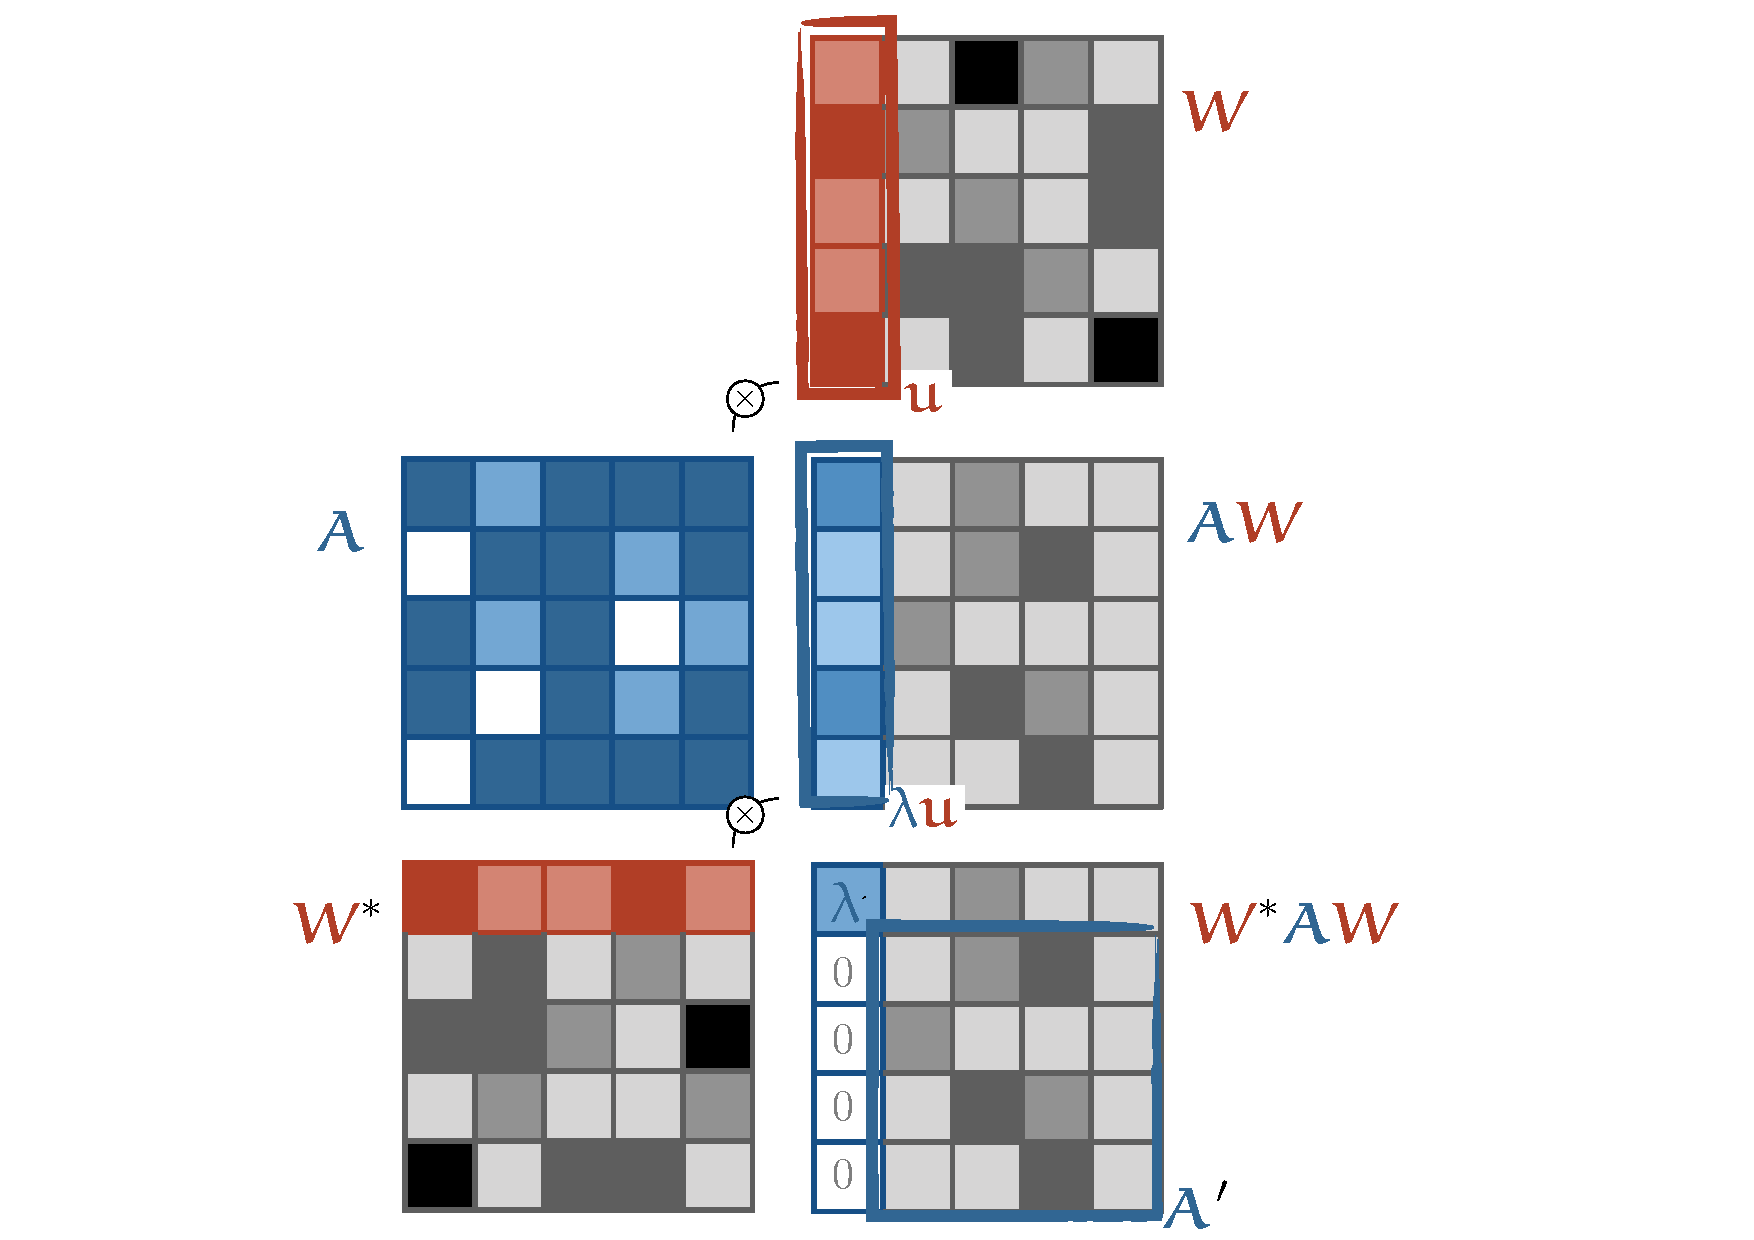
\includegraphics[width=0.65\textwidth]{./images/pca-3/schur-1.pdf}
	}
\end{figure}

%<figure class="centering">
%<img src="/images/pca-3/schur-1.svg" class="three-quarters">
%</figure>

Call this matrix \(\mbR\) (note that it is not triangular yet). So far we have shown that \(\rc{\mbW}^{*}\bc{\mbA}\rc{\mbW} = \mbR\), or if we multiply both sides by \(\rc{\mbW}^{*}\) and \(\rc{\mbW}\), that \(\bc{\mbA} = \rc{\mbW}\mbR\rc{\mbW}^*\).

Call \(\mbR\)'s bottom-right block \(\bc{\mbA}'\) as indicated in the image. \(\bc{\mbA}'\) is an \(n-1 \times n-1\) matrix, so by the assumption made above, it can be factorized: \(\bc{\mbA}' = \rc{\mbV}\bc{\mbQ}\rc{\mbV}^*\), with \(\rc{\mbV}\) unitary and \(\bc{\mbQ}\) upper triangular.

Now note that if we extend the matrix \(\rc{\mbV}\) to an \(n \times n\) matrix as follows

\[
\rc{\mbV}' = \begin{pmatrix}
~1 & 0 \ldots 0 \\
\begin{matrix}
~0\\ \vdots \\ 0
\end{matrix} 
& 
\rc{\mbV}
\end{pmatrix}
\]

we can move it out of the submatrix \(\bc{\mbA}'\), so that

\[
\bc{\mbA} = \rc{\mbW}\rc{\mbV}'\begin{pmatrix}
~\bc{\lambda} & *\;\ldots\; * \\
\begin{matrix}
~0\\ \vdots \\ 0
\end{matrix} 
& 
\mbQ
\end{pmatrix}\rc{\mbV}'^*\rc{\mbW}^*
\]

with the \(*\)'s representing arbitrary values.

We call the matrix in the middle \(\bc{\mbT}\). Note that this is now upper triangular. Note also that \(\rc{\mbV}'\) is unitary, since the column we added is a unit vector, and it's orthogonal to all other columns. Let \(\rc{\mbU} = \rc{\mbW}\rc{\mbV}'\). Since \(\rc{\mbW}\) and \(\rc{\mbV}'\) are unitary, their product is as well, and with that we have


\[
\bc{\mbA} = \rc{\mbU}\bc{\mbT}\rc{\mbU}^*
\]

proving the theorem. \hfill\qed

\end{proof}

\index{Schur decomposition!proof|)}


The important thing about the Schur decomposition is that it \emph{always works}. No matter what kind of square matrix we feed it, real or complex valued, with or without real eigenvalues, symmetric or asymmetric, singular or invertible, we always get a Schur decomposition out of it.

With this result in hand, the main difficulty of proving the spectral theorem is solved. We simply need to look at how the Schur decomposition behaves if we feed it a real-valued symmetric matrix

\subsection{Proof of the spectral theorem}

\index{Spectral theorem!proof|(}

\begin{theorem}[The spectral theorem] A matrix is orthogonally diagonalizable if and only if it is symmetric.
\end{theorem}
\begin{proof}
We will prove the two directions separately.

\paragraph{(1) If a real-valued matrix \(\bc{\mbA}\) is orth. diagonalizable, it must be symmetric.} Note that in an orthogonal diagonalization we have \(\bc{\mbD} = \bc{\mbD}^T\) because \(\bc{\mbD}\) is diagonal. Thus, if \(\bc{\mbA}\) is orthogonally diagonalizable, we know that 

\[
\bc{\mbA} = \rc{\mbP}\bc{\mbD}\rc{\mbP}^T = \rc{\mbP}^{T^T}\bc{\mbD}^T\rc{\mbP}^T = (\rc{\mbP}\bc{\mbD}\rc{\mbP}^T)^T = \bc{\mbA}^T 
\]

which implies that \(\bc{\mbA}\) is symmetric.

\paragraph{(2) If a real-valued matrix \(\bc{\mbA}\) is symmetric, it must be orth. diagonalizable.} For this direction, we need the Schur decomposition. By assumption \(\bc{\mbA}\) is symmetric and real-valued, so that \(\bc{\mbA}^* = \bc{\mbA}^T = \bc{\mbA}\). Let \(\bc{\mbA} = \rc{\mbU}\bc{\mbT}\rc{\mbU}^*\) be its Schur decomposition. 

\begin{aside}Note that we have assumed that \(\bc{\mbA}\) is real-valued, but \(\rc{\mbU}\) and \(\bc{\mbT}\) could still contain complex values.\end{aside}

From the symmetry of \(\bc{\mbA}\), we have \(\rc{\mbU}\bc{\mbT}\rc{\mbU}^* = (\rc{\mbU}\bc{\mbT}\rc{\mbU}^*)^* = \rc{\mbU}\bc{\mbT}^*\rc{\mbU}^*\), so \(\bc{\mbT} = \bc{\mbT}^*\). This tells us two things. First that all values off the diagonal are zero (remember that \(\bc{\mbT}\) is upper triangular), so \(\bc{\mbT}\) is actually diagonal. Second, that the values on the diagonal are equal to their own conjugate so they must be real values. 

This gives us a real-valued diagonalization \(\bc{\mbA} = \rc{\mbU}\bc{\mbT}\rc{\mbU}^*\). But what about the matrix \(\rc{\mbU}\)? Could that still contain complex values? It could, but knowing that \(\bc{\mbA}\) is real-valued, and so are the diagonal values of \(\bc{\mbT}\), we can perform the Schur decomposition specifically so that \(\rc{\mbU}\) ends up real valued as well.

\noindent Follow the construction of the Schur decomposition. In the \textbf{base case}, \(\rc{\mbU}\) is real-valued by definition. In the \textbf{inductive step}, assume that we can choose \(\rc{\mbV}\) real-valued for the case \(n-1\). When we choose the eigenvector for \(\bc{\lambda}\), we choose a real eigenvector. These always exist for real eigenvalues (proof in the appendix). When we choose the other columns of \(\rc{\mbW}\) we choose real valued vectors as well.

This means that \(\rc{\mbW}\) and \(\rc{\mbV}'\) are real, so their product \(\rc{\mbU}\) is real as well.

That completes the proof: if we perform the Schur decomposition in such a way that we choose real vectors for \(\rc{\mbW}\) where possible, the decomposition of a symmetric matrix gives us a diagonal real-valued matrix \(\bc{\mbT}\) and an orthogonal matrix \(\rc{\mbU}\). \hfill\qed
\end{proof}

\index{Spectral theorem!proof|)}

%\section{Conclusion}

It's been a long road, but we have finally reached the end. It's worth looking back at all the preliminaries we discussed, and briefly seeing why exactly they were necessary to show this result. Let's retrace our steps in reverse order.

The last thing we discussed, before the proof of the spectral theorem was the \textbf{Schur decomposition}. Its usefulness was clear: the Schur decomposition \emph{is} the eigendecomposition, if we're careful about its construction. The main benefit of the Schur decomposition is that it always works. With the real-valued eigendecomposition, we knew that it sometimes exists and sometimes doesn't. From that perspective it's very difficult to characterize the set of matrices for which it exists. The Schur decomposition allowed us to zoom out to the set of all matrices, so that we could ask what the decomposition looks like for real-valued, symmetric matrices.

The \textbf{complex numbers} make this possible. Filling matrices and vectors with complex numbers gives us a Schur decomposition that always works. The key to this is that the construction of the Schur decomposition requires us to pick one eigenvalue and corresponding eigenvector for various matrices. If we allow for complex eigenvalues, we ensure that this is  always possible.

This result, that every \(n \times n\) matrix has \(n\) eigenvalues if complex values are allowed, follows from two ideas. The first is the the \textbf{characteristic polynomial}. This is an \(n\)-th order polynomial, constructed from an \(n \times n\) matrix \(\bc{\mbA}\), that is zero, exactly when the \textbf{determinant} of \(\bc{\mbA} - \bc{\lambda}\mbI\) is zero. This means that the roots of the characteristic polynomial are the eigenvalues. The second idea is the \textbf{fundamental theorem of algebra} which tells us that every \(n\)-th order polynomial has exactly \(n\) roots in the complex plane, counting multiplicities. 

That gives us the spectral theorem and, as we saw in the last part, the spectral theorem gives us principal component analysis.

Now that we know how PCA works, why it works, and we have a thorough understanding of the spectral theorem, there is only one question left: \textbf{how do we implement it?} There are a couple of ways to go about this, but the best option by far is to make use of the singular value decomposition (SVD). This is a very versatile operation, which has many uses beyond the implementation of PCA. We will dig into the SVD into the next chapter.

\index{Singular value decomposition}

